\documentclass[a4paper,11pt]{report}
\usepackage{fullpage}

\usepackage{"../../info/packages"}
\usepackage{"../../info/nomenclature"}

\usepackage{scalerel}
\usepackage{subfiles}

\newcommand{\xvecdot}{\dot{\xvec}}
\newcommand{\xdot}{\dot{x}}
\newcommand{\qvecdot}{\dot{\qvec}}
\newcommand{\qdot}{\dot{q}}

\setlength{\cellspacetoplimit}{3pt}
\setlength{\cellspacebottomlimit}{3pt}

\title{Plasma Physics and Laser-driven Plasmas}
\author{Alejandro Campos}

\begin{document}
\maketitle
\tableofcontents

%%%%%%%%%%%%%%%%%%%%%%%%%%%%%%%%%%%%%%%%%%%%%%%%%%%%%%%%%%%%%%%%%%%%%%%%%
\part{Fundamentals of plasma physics}
%%%%%%%%%%%%%%%%%%%%%%%%%%%%%%%%%%%%%%%%%%%%%%%%%%%%%%%%%%%%%%%%%%%%%%%%%

%########################################################################
\chapter{Governing equations}
%########################################################################

%------------------------------------------------------------------------
\section{Particle description}
%------------------------------------------------------------------------
\begin{table}[H]
    \renewcommand{\arraystretch}{1.5}
    \centering
    \caption{Various coordinates of classical mechanics. }
    \label{tb:classical_mechanics_coordinates}
     \begin{tabular}{|l|l|l|}
        \hline
        Classical coordinates & $\xvec(t)$ & $\vvec(t)$ \\
        \hline
        Generalized coordinates  & $\qvec$ & $\qvecdot$ \\
        \hline
        Canonical coordinates & $\qvec$ & $\pvec$ \\
        \hline
        Time-dependent canonical coordinates & $\tilde{\qvec}(t)$ & $ \tilde{\pvec}(t)$ \\
        \hline
     \end{tabular}
\end{table}
    
%--------------------------------------------
\subsection{Lagrangian mechanics}
%--------------------------------------------
    
\begin{itemize}
    \item Define the position $\xvec = \xvec(t)$ and velocity $\vvec = \vvec(t)$ of a particle. 
    
    \item Define the Lagrangian as $L = L(\qvec, \qvecdot,t)$, where $\qvec$ and $\qvecdot$ are the generalized position and generalized velocity, respectively. 
    
    \item The equations of motion are obtained from the Euler-Lagrange equation, which is 
    \begin{equation}
    \frac{d}{dt} \left [ \left ( \frac{\partial L}{\partial \qdot_i } \right )_{\qvec =  \xvec, \qvecdot = \vvec }  \right] = \left ( \frac{\partial L}{\partial q_i} \right )_{ \qvec =  \xvec, \qvecdot = \vvec} .
    \end{equation}
    
    \item For example, the Lagrangian of a particle in an electromagnetic field where $\phi = \phi(\qvec,t)$ is the electric potential and $\Avec = \Avec(\qvec,t)$ is the magnetic potential, is
    \begin{equation}
    L = \frac{1}{2} m \qdot_i \qdot_i + e \qdot_i A_i - e\phi.
    \end{equation}
    The derivatives in the Euler-Lagrange equation are
    \begin{equation}
    \frac{\partial L}{\partial q_i} = e \qdot_j \frac{\partial A_j }{\partial q_i} - e \frac{\partial \phi}{ \partial q_i}
    \end{equation}
    \begin{equation}
    \frac{\partial L}{\partial \qdot_i} = m \qdot_i + e A_i 
    \end{equation}
    \begin{align}
    \frac{d}{dt}\left [ \left ( \frac{\partial L}{\partial \qdot_i } \right )_{\qvec =  \xvec, \qvecdot= \vvec }  \right] &= \frac{d}{dt} \left [ m v_i + e A_i(\xvec,t) \right ] \nonumber \\
    &= m \frac{ d v_i}{dt} + e v_j \left (\frac{\partial A_i}{\partial q_j} \right )_{\qvec = \xvec} +  e \left (\frac{\partial A_i}{\partial t} \right )_{\qvec = \xvec} .
    \end{align}
    Thus, the Euler-Lagrange equation becomes
    \begin{equation}
    \label{eq:lag_mech_tensor_lorentz}
    m \frac{ d v_i}{dt} = \left ( - e v_j \frac{\partial A_i}{\partial q_j} - e\frac{\partial A_i}{\partial t} + e v_j \frac{\partial A_j }{\partial q_i} - e \frac{\partial \phi}{ \partial q_i}\right )_{\qvec = \xvec}.
    \end{equation}
    In vector notation, this is written as
    \begin{equation}
        m \frac{d \vvec}{dt} = \left(-e\vvec \cdot \nabla_q \Avec - e \frac{\partial \Avec}{\partial t} + e \nabla_q (\vvec \cdot \Avec) - e \nabla_q \phi \right)_{\qvec = \xvec}.
    \end{equation}
    Using the vector identity (4) from Griffiths book, the above can be expressed as
    \begin{equation}
    m \frac{d\vvec}{dt} = e \left ( \Evec + \vvec \times \Bvec \right)_{\qvec = \xvec},
    \end{equation}
    where $\Evec = \Evec(\qvec,t)$ and $\Bvec = \Bvec(\qvec,t)$.
\end{itemize}
    
%--------------------------------------------
\subsection{Hamiltonian mechanics}
%--------------------------------------------
\begin{itemize}
    \item Define the Hamiltonian as $H = H(\qvec, \pvec, t)$, where $\qvec$ and $\pvec$ are the canonical position and momentum. For all purposes here, the canonical position is the same as the generalized position.
    
    \item The Hamiltonian is obtained from the Lagrangian using
    \begin{equation}
    H = \left ( \qvecdot \cdot \pvec - L \right)_{\qvecdot = \fvec(\qvec, \pvec)},
    \end{equation} 
    where the dependency of $\qvecdot$ on $\qvec$ and $\pvec$ is obtained from evaluating
    \begin{equation}
    \label{eq:v_from_qp}
    \pvec = \frac{ \partial L}{\partial \qvecdot}.
    \end{equation}
    
    \item For example, for a particle in an electromagnetic field we have
    \begin{equation}
    H = \left [ \qdot_i p_i - \left ( \frac{1}{2} m \qdot_i \qdot_i + e \qdot_i A_i - e\phi \right ) \right]_{\qvecdot = f(\qvec, \pvec)}. 
    \end{equation}
    Evaluating \cref{eq:v_from_qp} gives $ p_i = m \qdot_i + e A_i $, which allows us to express $\qvecdot$ in terms of $\qvec$ and $\pvec$ as $\qdot_i = \frac{1}{m} (p_i - eA_i )$. Thus
    \begin{align}
    H &= \frac{1}{m} (p_i - eA_i)p_i - \frac{1}{2m} (p_i - eA_i) (p_i-eA_i) - e\frac{1}{m} (p_i -eA_i) A_i + e\phi \nonumber \\
    & = \frac{1}{2m} (p_i -eA_i) (p_i -eA_i) + e\phi.
    \end{align}
    
    \item We introduce the variables $\tilde{\qvec} = \tilde{\qvec}(t)$ and $\tilde{\pvec} = \tilde{\pvec}(t)$, which are defined by
    \begin{align}
    \tilde{\qvec} &= \xvec \\ 
    \tilde{\pvec} & = \left ( \frac{\partial L}{\partial \qvecdot} \right)_{\qvec = \xvec, \qvecdot = \vvec}
    \end{align}
    
    \item The equations of motion are obtained from
    \begin{align}
    \frac{d \tilde{q}_i}{dt} &= \left ( \frac{ \partial H}{\partial p_i} \right )_{\qvec = \tilde{\qvec}, \pvec = \tilde{\pvec}} \\
    \frac{d \tilde{p}_i}{dt} & = -\left ( \frac{ \partial H}{\partial q_i} \right )_{\qvec = \tilde{\qvec}, \pvec = \tilde{\pvec}} \label{eq:hamil_p}
    \end{align}
    
    \item For example, for a particle in an electromagnetic field we have
    \begin{equation}
    \tilde{p}_i = mv_i + e A_i(\xvec,t)
    \end{equation}
    and thus
    \begin{align}
    \frac{d \tilde{p}_i}{dt} & = m \frac{d v_i}{dt} + e v_j \left ( \frac{\partial A_i}{\partial q_j} \right)_{\qvec = \xvec} + e \left ( \frac{ \partial A_i}{\partial t} \right)_{\qvec = \xvec}.
    \end{align}
    \begin{align}
    \frac{\partial H}{\partial q_i} &= \frac{\partial}{\partial q_i} \left [ \frac{1}{2m} (p_j -eA_j) (p_j -eA_j) + e\phi \right] \nonumber \\
    & = \frac{1}{m} (p_j -eA_j) \frac{\partial}{\partial q_i} (p_j - eA_j) + e\frac{\partial \phi}{\partial q_i} \nonumber \\
    &  = -\frac{e}{m} (p_j - eA_j) \frac{\partial A_j}{\partial q_i} + e \frac{\partial \phi}{\partial q_i}
    \end{align}
    \begin{align}
    \left ( \frac{ \partial H}{\partial q_i} \right )_{\qvec = \tilde{\qvec}, \pvec = \tilde{\pvec}} &= -\frac{e}{m} \left [ m v_j + eA_j(\xvec,t) - eA_j(\xvec,t) \right ] \left ( \frac{\partial A_j}{\partial q_i} \right)_{\qvec = \xvec} + e \left ( \frac{\partial \phi}{\partial q_i} \right)_{\qvec = \xvec} \nonumber \\
    & = \left( -e v_j \frac{\partial A_j}{\partial q_i} + e \frac{ \partial \phi}{\partial q_i} \right)_{\qvec = \xvec} .
    \end{align}
    
    \Cref{eq:hamil_p} thus leads to
    \begin{equation}
    m \frac{d v_i}{dt} = \left ( -e v_j \frac{ \partial A_i}{\partial q_j} - e \frac{ \partial A_i}{\partial t} + e v_j \frac{ \partial A_j}{\partial q_i} - e \frac{ \partial \phi}{\partial q_i} \right)_{\qvec = \xvec}.
    \end{equation}
    This is the same as \cref{eq:lag_mech_tensor_lorentz} and thus, as shown before, the above can be expressed as
    \begin{equation}
    \label{eq:single_particle_classical_mechanics}
    m \frac{d \vvec}{dt} = e \left ( \Evec + \vvec \times \Bvec \right)_{\qvec = \xvec}.
    \end{equation}
    
\end{itemize}

%------------------------------------------------------------------------
\section{Kinetic description}
%------------------------------------------------------------------------
We denote the distribution function for a species $s$ as $f_s = f_s(\rvec, \vvec, t)$, where $\rvec$ and $\vvec$ are the sample space variables for position and velocity. Note that the distribution function is appropriately normalized such that
\begin{equation}
\int f_s \, d\rvec d\vvec = N_s,
\end{equation}
where $N_s$ is the total number of particles corresponding to species $s$. 

The dynamics of a plasma can be characterized by the Boltzmann evolution equation for the distribution function of $M$ species along with Maxwell's equations
\begin{equation}
\label{eq:kinetic_equation}
\frac{\partial f_s}{\partial t} + \vvec \cdot \nabla f_s + \frac{Z_s e}{m_s} ( \Evec + \vvec \times \Bvec ) \cdot \nabla_v f_s = C_s + S_s
\end{equation}
\begin{equation}
\label{eq:maxwell_3}
\nabla \cdot \Evec = \frac{\rho_q}{\epsilon_0} 
\end{equation}
\begin{equation}
\label{eq:maxwell_4}
\nabla \cdot \Bvec = 0
\end{equation}
\begin{equation}
\label{eq:maxwell_1}
\nabla \times \Evec = -\frac{ \partial \Bvec}{\partial t}
\end{equation}
\begin{equation}
\label{eq:maxwell_2}
\nabla \times \Bvec = \mu_0 \Jvec + \mu_0 \epsilon_0 \frac{\partial \Evec}{\partial t}
\end{equation}
\begin{equation}
\Jvec = \sum_s^M Z_s e \int \vvec f_s \, d\vvec
\end{equation}
\begin{equation}
\rho_q = \sum_s^M Z_s e \int f_s \, d\vvec.
\end{equation}
In the above, 
\begin{itemize}
\item $m_s$ is the species mass
\item $e$ is the charge
\item $Z_s$ the charge number
\item $\Jvec = \Jvec(\rvec,t)$ the charge current
\item $\rho_q = \rho_q(\rvec,t)$ the charge density
\item $\Evec = \Evec(\rvec,t)$ the electric field
\item $\Bvec = \Bvec(\rvec,t)$ the magnetic field.
\end{itemize}
The terms $C_s$ and $S_s$ represent collision and source terms.

If we express the collision term in the usual way, that is $C_s = \sum_r^M C_{s r}$, then we can make the following statements:
\begin{enumerate}
\item Conservation of particles:
\begin{equation}
    \label{eq:coll_cons_particles}
    \int C_{ss} \, d\vvec = 0 \quad \forall s \qquad \qquad
    \int C_{sr} \,d\vvec = 0 \quad \forall s, r | r \ne s.
\end{equation}

\item Conservation of momentum:
\begin{equation}
    \label{eq:coll_cons_momentum}
    \int m_s \vvec C_{ss} \, d\vvec = 0 \quad \forall s \qquad \qquad \sum_s^M \sum_{r, r \ne s}^M \int m_s \vvec C_{sr} d\vvec = 0.
\end{equation}

\item Conservation of energy:
\begin{equation}
    \label{eq:coll_cons_energy}
    \int \frac{1}{2} m_s v^2 C_{ss} \, d\vvec = 0 \quad \forall s \qquad \qquad \sum_s^M \sum_{r, r \ne s}^M \int \frac{1}{2} m_s v^2 C_{sr} \, d\vvec = 0.
\end{equation}

\end{enumerate}

%------------------------------------------------------------------------
\section{Fluid description}
%------------------------------------------------------------------------
We now define the particle density $n_s = n_s(\rvec,t)$, the fluid velocity $\uvec_s = \uvec_s(\rvec,t)$ and the fluid energy per unit mass $E_s = E_s(\rvec,t)$ as follows
\begin{align}
n_s &= \int f_s \, d\vvec \\
\uvec_s &= \frac{1}{n_s} \int \vvec f_s \, d\vvec \\
E_s &= \frac{1}{n_s} \int \frac{1}{2} v^2 f_s \, d\vvec.
\end{align}
Their evolution equations are obtained by taking the appropriate moments of the Boltzmann plasma equation. Before doing so, we re-write the Boltzmann equation as
\begin{equation}
\label{eq:boltz_mod}
\frac{\partial f_s}{\partial t} + \nabla \cdot (\vvec f_s) + \nabla_v \cdot \left [ \frac{Z_s e}{m_s} ( \Evec + \vvec \times \Bvec ) f_s \right ] = C_s + S_s
\end{equation}

%--------------------------------------------
\subsection{Mass}
%--------------------------------------------
Integrating \cref{eq:boltz_mod} over all $\vvec$ we obtain
%\begin{empheq}[box=\widefbox]{equation}
\begin{equation}
\frac{\partial n_s}{\partial t} + \nabla \cdot \left ( n_s \uvec_s \right ) = \hat{S}_s
\end{equation}
%\end{empheq}
where 
\begin{equation}
\hat{S}_s = \int S_s \, d\vvec
\end{equation}
is an external source of mass.

%--------------------------------------------
\subsection{Momentum}
%--------------------------------------------
Multiplying \cref{eq:boltz_mod} by $\vvec$ and then integrating over all $\vvec$ leads to
\begin{multline}
\label{eq:mom_derv_1}
\frac{\partial n_s \uvec_s}{\partial t} + \nabla \cdot \left ( \int \vvec \vvec f_s \, d\vvec \right) + \int \nabla_v \cdot \left [ \vvec \frac{Z_s e}{m_s} ( \Evec + \vvec \times \Bvec ) f_s \right ] - \nabla_v \vvec \cdot \left [ \frac{Z_s e}{m_s} ( \Evec + \vvec \times \Bvec ) f_s \right ] \, d\vvec =\\
\sum_{r, r \ne s}^M \int \vvec C_{s r} \, d\vvec + \int \vvec S_s \, d\vvec.
\end{multline}
We note that the third term in \cref{eq:mom_derv_1} is zero since we are integrating over all space, and that $\nabla_v \vvec$ is the identity matrix. We thus have
\begin{multline}
\label{eq:mom_derv_2}
\frac{\partial n_s \uvec_s}{\partial t} + \nabla \cdot \left ( \int \vvec \vvec f_s \, d\vvec \right) - \frac{Z_s e n_s}{m_s} ( \Evec + \uvec_s \times \Bvec ) =\\
\sum_{r, r \ne s}^M \int \vvec C_{s r} \, d\vvec + \int \vvec S_s \, d\vvec.
\end{multline}

To proceed, we decompose $\vvec$ into a mean and a fluctuation, that is, $\vvec = \uvec_s + \wvec_s$. Using this decomposition 
\begin{equation}
\label{eq:identity_vv}
\int \vvec \vvec f_s \, d\vvec = \int ( \uvec_s \uvec_s + 2 \uvec_s \wvec_s + \wvec_s \wvec_s) f_s \, d\vvec = n_s \uvec_s \uvec_s + \int \wvec_s \wvec_s f_s \, d\vvec.
\end{equation}
Thus, \cref{eq:mom_derv_2} becomes
\begin{multline}
\label{eq:mom_derv_3}
\frac{\partial n_s \uvec_s}{\partial t} + \nabla \cdot \left ( n_s \uvec_s \uvec_s \right) - \frac{Z_s e n_s}{m_s} ( \Evec + \uvec_s \times \Bvec ) = -\nabla \cdot \int \wvec_s \wvec_s f_s d\vvec + \\
\sum_{r, r \ne s}^M \int \vvec C_{s r} \, d\vvec + \int \vvec S_s \, d\vvec.
\end{multline}
Conservation of particles is used to modify the collisional term as follows
\begin{align}
    \label{eq:mom_collision_expansion}
    \sum_{r,r \ne s}^M \int \vvec C_{s r} \, d\vvec 
    &= \sum_{r,r \ne s}^M \int (\uvec_s + \wvec_s) C_{s r} \, d\vvec \nonumber \\
    &= \sum_{r,r \ne s}^M \int \wvec_s C_{s r} \, d\vvec 
\end{align}
Thus, we now have
\begin{multline}
\label{eq:mom_derv_4}
\frac{\partial n_s \uvec_s}{\partial t} + \nabla \cdot \left ( n_s \uvec_s \uvec_s \right) - \frac{Z_s e n_s}{m_s} ( \Evec + \uvec_s \times \Bvec ) = -\nabla \cdot \int \wvec_s \wvec_s f_s d\vvec + \\
\sum_{r, r \ne s}^M \int \wvec_s C_{s r} \, d\vvec + \int \vvec S_s \, d\vvec.
\end{multline}

Multiplying by mass leads to the following equation
%\begin{empheq}[box=\widefbox]{equation}
\begin{equation}
\label{eq:mom_derv_5}
\frac{\partial m_s n_s \uvec_s}{\partial t} + \nabla \cdot \left ( m_s n_s \uvec_s \uvec_s \right) - Z_s e n_s ( \Evec + \uvec_s \times \Bvec ) = \nabla \cdot \boldsymbol{\sigma}_s + \Rvec_s + \hat{\Mvec}_s,
\end{equation}
%\end{empheq}
where the stress tensor is
\begin{equation}
\boldsymbol{\sigma}_s = -\int m_s \wvec_s \wvec_s f_s \, d\vvec,
\end{equation}
the momentum transferred between unlike particles due to friction of collisions is
\begin{equation}
\Rvec_s = \sum_{r, r \ne s}^M \int m_s \wvec_s C_{s r} \, d\vvec,
\end{equation}
and the external source of momentum is
\begin{equation}
\hat{\Mvec}_s = \int m_s \vvec S_s \, d\vvec.
\end{equation}
 
The stress tensor is typically decomposed into isotropic $p_s$ and anisotropic (shear) $\tvec_s$ tensors as follows
\begin{equation}
\boldsymbol{\sigma}_s = - p_s \Ivec + \tvec_s,
\end{equation}
where $p_s$ is given by
\begin{equation}
p_s = \frac{1}{3} \int m_s (\wvec_s \cdot \wvec_s) f_s d\vvec.
\end{equation}
Thus, conservation of momentum becomes
\begin{equation}
\label{eq:mom_derv_6}
\frac{\partial m_s n_s \uvec_s}{\partial t} + \nabla \cdot \left ( m_s n_s \uvec_s \uvec_s \right) - Z_s e n_s ( \Evec + \uvec_s \times \Bvec ) = - \nabla p_s + \nabla \cdot \tvec_s + \Rvec_s + \hat{\Mvec}_s.
\end{equation}

%--------------------------------------------
\subsection{Energy}
%--------------------------------------------
Multiplying \cref{eq:boltz_mod} by $\frac{1}{2} v^2$ and then integrating over all $\vvec$ leads to
\begin{multline}
\label{eq:energy_derv_1}
\frac{\partial n_s E_s}{\partial t} + \nabla \cdot \left [ \int \frac{1}{2} (\vvec \cdot \vvec) \vvec f_s \, d\vvec \right ] + \int \nabla_v \cdot \left [ \frac{1}{2} (\vvec \cdot \vvec) \frac{Z_s e}{m_s} ( \Evec + \vvec \times \Bvec ) f_s \right ] \\
- \nabla_v \left [ \frac{1}{2} (\vvec \cdot \vvec) \right ] \cdot \left [ \frac{Z_s e}{m_s} ( \Evec + \vvec \times \Bvec ) f_s \right ] \, d\vvec = \sum_{r, r \ne s}^M \int \frac{1}{2} (\vvec \cdot \vvec) C_{s r} \, d\vvec + \int \frac{1}{2} (\vvec \cdot \vvec) S_s \, d\vvec.
\end{multline}
We note that the third term above is zero since we are integrating over all space, and that $\nabla_v [ 1/2 (\vvec \cdot \vvec ) ] = \vvec$. Thus, we have
\begin{multline}
\label{eq:energy_derv_2}
\frac{\partial n_s E_s}{\partial t} + \nabla \cdot \left [ \int \frac{1}{2} (\vvec \cdot \vvec) \vvec f_s \, d\vvec \right ] - \frac{Z_s e n_s}{m_s} \Evec \cdot \uvec_s =\\
\sum_{r, r \ne s}^M \int \frac{1}{2} (\vvec \cdot \vvec) C_{s r} \, d\vvec + \int \frac{1}{2} (\vvec \cdot \vvec) S_s \, d\vvec.
\end{multline}

To proceed with the derivation we first note that
\begin{multline}
\int \frac{1}{2} (\vvec \cdot \vvec) \vvec f_s \, d\vvec = \int \frac{1}{2} (\vvec \cdot \vvec) (\uvec_s + \wvec_s) f_s \, d\vvec = n_s E_s \uvec_s + \int \frac{1}{2} (\vvec \cdot \vvec ) \wvec_s f_s \, d\vvec
\end{multline}
The last term on the right-hand side above can be re-written as
\begin{align}
\int \frac{1}{2} ( \vvec \cdot \vvec ) \wvec_s f_s \, d\vvec &= \int \frac{1}{2} ( \uvec_s \cdot \uvec_s + 2\uvec_s \cdot \wvec_s + \wvec_s \cdot \wvec_s ) \wvec_s f_s \, d\vvec \\
& =  \uvec_s \cdot \int \wvec_s \wvec_s f_s \, d\vvec + \int \frac{1}{2} ( \wvec_s \cdot \wvec_s ) \wvec_s f_s \, d\vvec.
\end{align}
Using the expressions above, \cref{eq:energy_derv_2} becomes
\begin{multline}
\label{eq:energy_derv_3}
\frac{\partial n_s E_s}{\partial t} + \nabla \cdot (n_s E_s \uvec_s ) - \frac{Z_s e n_s}{m_s} \Evec \cdot \uvec_s =  - \nabla \cdot \left ( \uvec_s \cdot \int \wvec_s \wvec_s f_s \, d\vvec \right ) - \nabla \cdot \int \frac{1}{2} ( \wvec_s \cdot \wvec_s ) \wvec_s f_s \, d\vvec\\
+ \sum_{r, r \ne s}^M \int \frac{1}{2} (\vvec \cdot \vvec) C_{s r} \, d\vvec + \int \frac{1}{2} (\vvec \cdot \vvec) S_s \, d\vvec.
\end{multline}
Conservation of particles is used to modify the collisional term as follows
\begin{align}
    \label{eq:energy_collision_expansion}
    \sum_{r,r \ne s}^M \int \frac{1}{2} (\vvec \cdot \vvec) C_{s r} \, d\vvec 
    &= \sum_{r,r \ne s}^M \int \frac{1}{2} [ (\uvec_s + \wvec_s) \cdot (\uvec_s + \wvec_s)] C_{s r} \, d\vvec \nonumber \\
    &= \uvec_s \cdot  \sum_{r,r \ne s}^M \int \wvec_s C_{s r} \, d\vvec + \sum_{r,r \ne s}^M \int \frac{1}{2} (\wvec_s \cdot \wvec_s) C_{s r} \, d\vvec 
\end{align}
Thus, we now have
\begin{multline}
\label{eq:energy_derv_4}
\frac{\partial n_s E_s}{\partial t} + \nabla \cdot (n_s E_s \uvec_s ) - \frac{Z_s e n_s}{m_s} \Evec \cdot \uvec_s = - \nabla \cdot \left ( \uvec_s \cdot \int \wvec_s \wvec_s f_s \, d\vvec  \right ) - \nabla \cdot \int \frac{1}{2} ( \wvec_s \cdot \wvec_s ) \wvec_s f_s \, d\vvec \\
+ \uvec_s \cdot \sum_{r,r \ne s}^M \int \wvec_s C_{s r} \, d\vvec + \sum_{r, r \ne s}^M \int \frac{1}{2} (\wvec_s \cdot \wvec_s) C_{s r} \, d\vvec + \int \frac{1}{2} (\vvec \cdot \vvec) S_s \, d\vvec.
\end{multline}

Multiplying by mass leads to the following equation
%\begin{empheq}[box=\widefbox]{multline}
\begin{multline}
\label{eq:energy_derv_5}
\frac{\partial m_s n_s E_s}{\partial t} + \nabla \cdot (m_s n_s E_s \uvec_s ) - Z_s e n_s \Evec \cdot \uvec_s = \nabla \cdot ( \uvec_s \cdot \boldsymbol{\sigma}_s ) - \nabla \cdot \qvec_s \\
+ \uvec_s \cdot \Rvec_s + Q_{s} + \hat{Q}_s, 
\end{multline}
%\end{empheq}
where heat flux due to random motion is
\begin{equation}
\qvec_s = \int \frac{1}{2} m_s (\wvec_s \cdot \wvec_s ) \wvec_s f_s \, d\vvec,
\end{equation}
the heat generated and transferred between unlike particles due to collisional dissipation is 
\begin{equation}
Q_{s} = \sum_{r,r \ne s}^M \int \frac{1}{2} m_s (\wvec_s \cdot \wvec_s) C_{s r} \, d\vvec,
\end{equation}
and the external source of energy is
\begin{equation}
\hat{Q}_s = \int \frac{1}{2} m_s (\vvec \cdot \vvec) S_s \, d\vvec.
\end{equation}

Using the decomposition for the stress tensor, the conservation of energy equation becomes
\begin{multline}
\label{eq:energy_derv_6}
\frac{\partial m_s n_s E_s}{\partial t} + \nabla \cdot (m_s n_s E_s \uvec_s + p_s \uvec_s ) - Z_s e n_s \Evec \cdot \uvec_s = \nabla \cdot ( \uvec_s \cdot \tvec_s ) - \nabla \cdot \qvec_s \\
+ \uvec_s \cdot \Rvec_s + Q_{s} + \hat{Q}_s, 
\end{multline}
We also note that the energy $m_s n_s E_s$ can be decomposed into internal and kinetic energies. Using the trace of the decomposition shown in \cref{eq:identity_vv} one obtains
\begin{align}
m_s n_s E_s & = \int \frac{1}{2} m_s (\vvec \cdot \vvec) f_s \, d\vvec \nonumber \\
& = \int \frac{1}{2} m_s (\wvec_s \cdot \wvec_s) f_s \, d\vvec + \frac{1}{2} m_s n_s (\uvec_s \cdot \uvec_s) \nonumber \\
& = \frac{3}{2} p_s + \frac{1}{2} m_s n_s (\uvec_s \cdot \uvec_s) \nonumber \\
& = \frac{3}{2} p_s + m_s n_s K_s.
\end{align}
where $K_s = \frac{1}{2} \uvec_s \cdot \uvec_s$ is the kinetic energy of species $s$.

%--------------------------------------------
\subsection{Kinetic and internal energies}
%--------------------------------------------
The equation for the kinetic energy is obtained by dotting \cref{eq:mom_derv_6} with $\uvec_s$. For this, we first show that
\begin{align}
    \uvec_s \cdot &\left [ \frac{\partial m_s n_s \uvec_s}{\partial t} + \nabla \cdot \left ( m_s n_s \uvec_s \uvec_s \right) \right ] \\
    & =\uvec_s \cdot \left \{ \left [ \frac{\partial m_s n_s }{\partial t} + \nabla \cdot \left ( m_s n_s \uvec_s \right) \right] \uvec_s  + m_s n_s \left ( \frac{\partial \uvec_s}{\partial t} + \uvec_s \cdot \nabla \uvec_s \right ) \right \}\\
    & =\uvec_s \cdot \left [ m_s \hat{S}_s \uvec_s  + m_s n_s \left ( \frac{\partial \uvec_s}{\partial t} + \uvec_s \cdot \nabla \uvec_s \right ) \right ] \\
    & =2m_s \hat{S}_s K_s + m_s n_s \left ( \frac{\partial K_s}{\partial t} + \uvec_s \cdot \nabla K_s \right) \\
    & =m_s \hat{S}_s K_s + \left [ \frac{\partial m_s n_s}{\partial t} + \nabla \cdot \left (m_s n_s \uvec_s \right ) \right] K_s + m_s n_s \left ( \frac{\partial K_s}{\partial t} + \uvec_s \cdot \nabla K_s \right) \\
    & =m_s \hat{S}_s K_s + \frac{\partial m_s n_s K_s}{\partial t} + \nabla \cdot ( m_s n_s K \uvec_s ).
\end{align}
Thus, the equation for the turbulent kinetic energy is
\begin{multline}
\frac{\partial m_s n_s K_s}{\partial t} + \nabla \cdot ( m_s n_s K \uvec_s ) - Z_s e n_s \Evec \cdot \uvec_s =\\
\nabla \cdot (\uvec_s \cdot \sigmavec_s ) - \sigmavec_s : \nabla \uvec_s + \uvec_s \cdot \Rvec_s + \uvec_s \cdot \hat{\Mvec}_s - m_s K_s \hat{S}_s .
\end{multline}
Subtracting the above equation from \cref{eq:energy_derv_6} leads to 
\begin{equation}
\frac{\partial}{\partial t} \left ( \frac{3}{2} p_s \right ) + \nabla \cdot \left ( \frac{3}{2} p_s \uvec_s \right ) = \sigmavec_s : \nabla \uvec_s - \nabla \cdot \qvec_s + Q_{s} + \hat{Q}_s - \uvec_s \cdot \hat{\Mvec}_s + m_s K_s \hat{S}_s .
\end{equation}

%--------------------------------------------
\subsection{Summary}
%--------------------------------------------
To summarize, we have,
\begin{itemize}
    \item Particle density
\begin{equation}
\label{eq:cons_mass}
    \frac{\partial n_s}{\partial t} + \nabla \cdot \left ( n_s \uvec_s \right ) = \hat{S}_s,
\end{equation}

    \item Momentum
\begin{equation}
\label{eq:cons_mom}
    \frac{\partial m_s n_s \uvec_s}{\partial t} + \nabla \cdot \left ( m_s n_s \uvec_s \uvec_s \right) - Z_s e n_s ( \Evec + \uvec_s \times \Bvec ) = \nabla \cdot \sigmavec_s + \Rvec_s + \hat{\Mvec}_s,
\end{equation}

    \item Total Energy
\begin{multline}
\label{eq:cons_te}
\frac{\partial m_s n_s E_s}{\partial t} + \nabla \cdot (m_s n_s E_s \uvec_s ) - Z_s e n_s \Evec \cdot \uvec_s = \nabla \cdot ( \uvec_s \cdot \sigmavec_s ) - \nabla \cdot \qvec_s \\
+ \uvec_s \cdot \Rvec_s + Q_{s} + \hat{Q}_s, 
\end{multline}
    
    \item Kinetic Energy
\begin{multline}
\label{eq:cons_ke}
\frac{\partial m_s n_s K_s}{\partial t} + \nabla \cdot ( m_s n_s K \uvec_s ) - Z_s e n_s \Evec \cdot \uvec_s =\\
\nabla \cdot (\uvec_s \cdot \sigmavec_s ) - \sigmavec_s : \nabla \uvec_s + \uvec_s \cdot \Rvec_s + \uvec_s \cdot \hat{\Mvec}_s - m_s K_s \hat{S}_s .
\end{multline}    
    
    \item Internal Energy
\begin{equation}
\label{eq:cons_ie}
    \frac{\partial}{\partial t} \left ( \frac{3}{2} p_s \right ) + \nabla \cdot \left ( \frac{3}{2} p_s \uvec_s \right ) = \sigmavec_s : \nabla \uvec_s - \nabla \cdot \qvec_s + Q_{s} + \hat{Q}_s - \uvec_s \cdot \hat{\Mvec}_s + m_s K_s \hat{S}_s .  
\end{equation}

\end{itemize}

%########################################################################
\chapter{Variants of the fluid model}
%########################################################################

%------------------------------------------------------------------------
\section{The multi-fluid model}
%------------------------------------------------------------------------
The following assumptions are used:
\begin{enumerate}
    \item No sources ($\hat{S}_s = \hat{\Mvec}_s = \hat{Q}_s = 0$ for all $s$).
\end{enumerate}

%--------------------------------------------
\subsection{Multi-material multi-fluid model}
%--------------------------------------------
We define a material $k$ as a collection of species $s$. Rather than labeling species using the subscript $s$, we'll use the subscript $k,i,s$ and $k,e$, where the former denotes the ion species $s$ that belongs to material $k$, and the latter denotes the electron species that belongs to material $k$. We also note that the number of ion species within a material will be denoted as $N_k$, and the total number of materials as $L$.

Thus, the governing equations are
\begin{equation}
    \label{eq:mf_mm_ni}
    \frac{\partial n_{k,i,s}}{\partial t} + \nabla \cdot \left ( n_{k,i,s} \uvec_{k,i,s} \right ) = 0,
\end{equation}
\begin{equation}
    \label{eq:mf_mm_ne}
    \frac{\partial n_{k,e}}{\partial t} + \nabla \cdot \left ( n_{k,e} \uvec_{k,e} \right ) = 0,
\end{equation}
\begin{equation}
    \label{eq:mf_mm_ui}
    \frac{\partial m_{k,i,s} n_{k,i,s} \uvec_{k,i,s}}{\partial t} + \nabla \cdot \left( m_{k,i,s} n_{k.i,s} \uvec_{k,i,s} \uvec_{k,i,s} \right) 
    - Z_{k,i,s} e n_{k,i,s} ( \Evec + \uvec_{k,i,s} \times \Bvec ) = \nabla \cdot \sigmavec_{k,i,s} + \Rvec_{k,i,s},
\end{equation}
\begin{equation}
    \label{eq:mf_mm_ue}
    \frac{\partial m_{k,e} n_{k,e} \uvec_{k,e}}{\partial t} + \nabla \cdot \left( m_{k,e} n_{k,e} \uvec_{k,e} \uvec_{k,e} \right) + e n_{k,e} ( \Evec + \uvec_{k,e} \times \Bvec ) = \nabla \cdot \sigmavec_{k,e} + \Rvec_{k,e},
\end{equation}
\begin{equation}
    \label{eq:mf_mm_iei}
    \frac{\partial}{\partial t} \left ( \frac{3}{2} p_{k,i,s} \right ) + \nabla \cdot \left ( \frac{3}{2} p_{k,i,s} \uvec_{k,i,s} \right ) = \sigmavec_{k,i,s} : \nabla \uvec_{k,i,s} - \nabla \cdot \qvec_{k,i,s} + Q_{k,i,s},
\end{equation}
\begin{equation}
    \label{eq:mf_mm_iee}
    \frac{\partial}{\partial t} \left ( \frac{3}{2} p_{k,e} \right ) + \nabla \cdot \left ( \frac{3}{2} p_{k,e} \uvec_{k,e} \right ) = \sigmavec_{k,e} : \nabla \uvec_{k,e} - \nabla \cdot \qvec_{k,e} + Q_{k,e},
\end{equation}
\begin{equation}
    \label{eq:mf_mm_maxwell_3}
    \nabla \cdot \Evec = \frac{\rho_q}{\epsilon_0},
\end{equation}
\begin{equation}
    \label{eq:mf_mm_maxwell_4}
    \nabla \cdot \Bvec = 0,
\end{equation}
\begin{equation}
    \label{eq:mf_mm_maxwell_1}
    \nabla \times \Evec = -\frac{ \partial \Bvec}{\partial t},
\end{equation}
\begin{equation}
    \label{eq:mf_mm_maxwell_2}
    \nabla \times \Bvec = \mu_0 \Jvec + \mu_0 \epsilon_0 \frac{\partial \Evec}{\partial t},
\end{equation}
\begin{equation}
    \label{eq:mf_mm_curr_density}
    \Jvec_k = e \left( \sum_s^{N_k} Z_{k,i,s} n_{k,i,s} \uvec_{k,i,s} - n_{k,e} \uvec_{k,e} \right),
\end{equation}
\begin{equation}
    \Jvec = \sum_k^L \Jvec_k
\end{equation}
\begin{equation}
    \label{eq:mf_mm_mass_density}
    \rho_{q,k} = e \left( \sum_s^N Z_{k,i,s} n_{k,i,s} - n_{e,k} \right),
\end{equation}
\begin{equation}
    \rho_q = \sum_k^L \rho_{q,k},
\end{equation}
\begin{equation}
    \label{eq:mf_mm_eos_ion}
    p_{k,i,s} = n_{k,i,s} k_B T_{k,i,s},
\end{equation}
\begin{equation}
    \label{eq:mf_mm_eos_elec}
    p_{k,e} = n_{k,e} k_B T_{k,e}.
\end{equation}

%--------------------------------------------
\subsection{Single-material multi-fluid model}
%--------------------------------------------
\label{sec:mf_np1fluid_equations}
The equations are the same as the multi-material formulation, but there is only one material now and hence the $k$ subscript can be dropped. Thus we have 
\begin{equation}
    \label{eq:mf_np1fluid_ni}
    \frac{\partial n_{i,s}}{\partial t} + \nabla \cdot \left ( n_{i,s} \uvec_{i,s} \right ) = 0,
\end{equation}
\begin{equation}
    \label{eq:mf_np1fluid_ne}
    \frac{\partial n_e}{\partial t} + \nabla \cdot \left ( n_e \uvec_e \right ) = 0,
\end{equation}
\begin{equation}
    \label{eq:mf_np1fluid_ui}
    \frac{\partial m_{i,s} n_{i,s} \uvec_{i,s}}{\partial t} + \nabla \cdot \left( m_{i,s} n_{i,s} \uvec_{i,s} \uvec_{i,s} \right) - Z_{i,s} e n_{i,s} ( \Evec + \uvec_{i,s} \times \Bvec ) = \nabla \cdot \sigmavec_{i,s} + \Rvec_{i,s},
\end{equation}
\begin{equation}
    \label{eq:mf_np1fluid_ue}
    \frac{\partial m_e n_e \uvec_e}{\partial t} + \nabla \cdot \left ( m_e n_e \uvec_e \uvec_e \right) + e n_e ( \Evec + \uvec_e \times \Bvec ) = \nabla \cdot \sigmavec_e + \Rvec_e,
\end{equation}
\begin{equation}
    \label{eq:mf_np1fluid_iei}
    \frac{\partial}{\partial t} \left ( \frac{3}{2} p_{i,s} \right ) + \nabla \cdot \left ( \frac{3}{2} p_{i,s} \uvec_{i,s} \right ) = \sigmavec_{i,s} : \nabla \uvec_{i,s} - \nabla \cdot \qvec_{i,s} + Q_{i,s},
\end{equation}
\begin{equation}
    \label{eq:mf_np1fluid_iee}
    \frac{\partial}{\partial t} \left ( \frac{3}{2} p_e \right ) + \nabla \cdot \left ( \frac{3}{2} p_e \uvec_e \right ) = \sigmavec_e : \nabla \uvec_e - \nabla \cdot \qvec_e + Q_e,
\end{equation}
\begin{equation}
    \label{eq:mf_np1fluid_maxwell_3}
    \nabla \cdot \Evec = \frac{\rho_q}{\epsilon_0},
\end{equation}
\begin{equation}
    \label{eq:mf_np1fluid_maxwell_4}
    \nabla \cdot \Bvec = 0,
\end{equation}
\begin{equation}
    \label{eq:mf_np1fluid_maxwell_1}
    \nabla \times \Evec = -\frac{ \partial \Bvec}{\partial t},
\end{equation}
\begin{equation}
    \label{eq:mf_np1fluid_maxwell_2}
    \nabla \times \Bvec = \mu_0 \Jvec + \mu_0 \epsilon_0 \frac{\partial \Evec}{\partial t},
\end{equation}
\begin{equation}
    \label{eq:mf_np1fluid_curr_density}
    \Jvec = e \left(\sum_s^N Z_{i,s} n_{i,s} \uvec_{i,s} - n_e \uvec_e \right),
\end{equation}
\begin{equation}
    \label{eq:mf_np1fluid_mass_density}
    \rho_q = e \left( \sum_s^N Z_{i,s} n_{i,s} - n_e \right),
\end{equation}
\begin{equation}
    \label{eq:mf_np1fluid_eos_ion}
    p_{i,s} = n_{i,s} k_B T_{i,s},
\end{equation}
\begin{equation}
    \label{eq:mf_np1fluid_eos_elec}
    p_e = n_e k_B T_e.
\end{equation}

%--------------------------------------------
\subsection{Single-material two-fluid model}
%--------------------------------------------
If there is only one ion species, then we have the two-fluid model
\label{sec:mf_2fluid_equations}
\begin{equation}
    \label{eq:mf_2fluid_ni}
    \frac{\partial n_i}{\partial t} + \nabla \cdot \left ( n_i \uvec_i \right ) = 0,
\end{equation}
\begin{equation}
    \label{eq:mf_2fluid_ne}
    \frac{\partial n_e}{\partial t} + \nabla \cdot \left ( n_e \uvec_e \right ) = 0,
\end{equation}
\begin{equation}
    \label{eq:mf_2fluid_ui}
    \frac{\partial m_i n_i \uvec_i}{\partial t} + \nabla \cdot \left ( m_i n_i \uvec_i \uvec_i \right) - Z e n_i ( \Evec + \uvec_i \times \Bvec ) = \nabla \cdot \sigmavec_i + \Rvec_i,
\end{equation}
\begin{equation}
    \label{eq:mf_2fluid_ue}
    \frac{\partial m_e n_e \uvec_e}{\partial t} + \nabla \cdot \left ( m_e n_e \uvec_e \uvec_e \right) + e n_e ( \Evec + \uvec_e \times \Bvec ) = \nabla \cdot \sigmavec_e + \Rvec_e,
\end{equation}
\begin{equation}
    \label{eq:mf_2fluid_iei}
    \frac{\partial}{\partial t} \left ( \frac{3}{2} p_i \right ) + \nabla \cdot \left ( \frac{3}{2} p_i \uvec_i \right ) = \sigmavec_i : \nabla \uvec_i - \nabla \cdot \qvec_i + Q_i,
\end{equation}
\begin{equation}
    \label{eq:mf_2fluid_iee}
    \frac{\partial}{\partial t} \left ( \frac{3}{2} p_e \right ) + \nabla \cdot \left ( \frac{3}{2} p_e \uvec_e \right ) = \sigmavec_e : \nabla \uvec_e - \nabla \cdot \qvec_e + Q_e,
\end{equation}
\begin{equation}
    \label{eq:mf_2fluid_maxwell_3}
    \nabla \cdot \Evec = \frac{\rho_q}{\epsilon_0},
\end{equation}
\begin{equation}
    \label{eq:mf_2fluid_maxwell_4}
    \nabla \cdot \Bvec = 0,
\end{equation}
\begin{equation}
    \label{eq:mf_2fluid_maxwell_1}
    \nabla \times \Evec = -\frac{ \partial \Bvec}{\partial t},
\end{equation}
\begin{equation}
    \label{eq:mf_2fluid_maxwell_2}
    \nabla \times \Bvec = \mu_0 \Jvec + \mu_0 \epsilon_0 \frac{\partial \Evec}{\partial t},
\end{equation}
\begin{equation}
    \label{eq:mf_2fluid_curr_density}
    \Jvec = e (Z n_i \uvec_i - n_e \uvec_e),
\end{equation}
\begin{equation}
    \label{eq:mf_2fluid_mass_density}
    \rho_q = e (Z n_i - n_e).
\end{equation}
\begin{equation}
    \label{eq:mf_2fluid_eos_ion}
    p_i = n_i k_B T_i,
\end{equation}
\begin{equation}
    \label{eq:mf_2fluid_eos_elec}
    p_e = n_e k_B T_e.
\end{equation}
These equations correspond to eq.\@ (2.22) in Freidberg's Ideal MHD book, but for ions that are not singly charged.

We can also introduce the following extra assumptions
\begin{enumerate}
    \item No stresses $\tvec_s$, heat flux $\qvec_s$, and collisions $\Rvec_s$, $Q_s$. This in itself would make the flow isentropic.
    \item The flow is not just isentropic but also homentropic. This allows for \cref{eq:pwaves_ion_pressure,eq:pwaves_electron_pressure} to hold across all space, not just along streamlines.
\end{enumerate}
With these, the governing equations become
\begin{equation}
    \label{eq:pwaves_ion_density}
    \frac{\partial n_i}{\partial t} + \nabla \cdot \left (n_i \uvec_i \right ) = 0,
\end{equation}
\begin{equation}
    \label{eq:pwaves_electron_density}
    \frac{\partial n_e}{\partial t} + \nabla \cdot \left (n_e \uvec_e \right ) = 0,
\end{equation}
\begin{equation}
    \label{eq:pwaves_ion_momentum}
    \frac{\partial m_i n_i \uvec_i}{\partial t} + \nabla \cdot \left ( m_i n_i \uvec_i \uvec_i \right ) - Ze n_i \left ( \Evec + \uvec_i \times \Bvec \right ) = -\nabla p_i,
\end{equation}
\begin{equation}
    \label{eq:pwaves_electron_momentum}
    \frac{\partial m_e n_e \uvec_e}{\partial t} + \nabla \cdot \left ( m_e n_e \uvec_e \uvec_e \right ) + e n_e \left ( \Evec + \uvec_e \times \Bvec \right ) = -\nabla p_e,
\end{equation}
\begin{equation}
    \label{eq:pwaves_ion_pressure}
    p_i = C_i n_i^{\gamma_i},
\end{equation}
\begin{equation}
    \label{eq:pwaves_electron_pressure}
    p_e = C_e n_e^{\gamma_e},
\end{equation}
\begin{equation}
    \label{eq:pwaves_maxwell_3}
    \nabla \cdot \Evec = \frac{\rho_q}{\epsilon_0},
\end{equation}
\begin{equation}
    \label{eq:p_waves_maxwell_4}
    \nabla \cdot \Bvec = 0,
\end{equation}
\begin{equation}
    \label{eq:p_waves_maxwell_1}
    \nabla \times \Evec = -\frac{ \partial \Bvec}{\partial t},
\end{equation}
\begin{equation}
    \label{eq:p_waves_maxwell_2}
    \nabla \times \Bvec = \mu_0 \Jvec + \mu_0 \epsilon_0 \frac{\partial \Evec}{\partial t},
\end{equation}
\begin{equation}
    \label{eq:p_waves_curr_density}
    \Jvec = e (Z n_i \uvec_i - n_e \uvec_e),
\end{equation}
\begin{equation}
    \label{eq:p_waves_mass_density}
    \rho_q = e (Z n_i - n_e),
\end{equation}
\begin{equation}
    p_i = n_i k_B T_i,
\end{equation}
\begin{equation}
    p_e = n_e k_B T_e.
\end{equation}

%------------------------------------------------------------------------
\section{Single-fluid formulation}
%------------------------------------------------------------------------
A single-fluid formulation is defined as that for which there is a single velocity vector. For the single-fluid formulation, we'll use the following assumptions
\begin{enumerate}
    \item $m_{k,e} \approx 0$ since $m_{k,e} \ll m_{k,i,s}$. \label{eq:sf_no_e_mass} 
    \item Quasi-neutrality, i.e.\@ $\sum_s^{N_k} Z_{k,i,s} n_{k,i,s} = n_{k,e}$. \label{eq:sf_quasi_neutrality}
\end{enumerate}

%--------------------------------------------
\subsection{Single-fluid variables}
%--------------------------------------------
To derive the single-fluid equations we first introduce a set of new variables. 

The total density $\rho$ is defined as
\begin{equation}
    \rho = m/V.
\end{equation}
The volume fraction $\eta_k$ and mass fraction $Y_k$ are defined as
\begin{equation}
    \eta_k = \frac{V_k}{V},
\end{equation}
\begin{equation}
    Y_k = \frac{m_k}{m}.
\end{equation}
Note that both $\eta_k$ and $Y_k$ sum up to one over all $k$. A new density is also introduced, namely $\rho_k$ which is defined as
\begin{equation}
    \rho_k= \frac{m_k}{V_k}.
\end{equation}
This can be expressed in terms of the other variables defined above by
\begin{equation}
    \rho_k = \rho \frac{Y_k}{\eta_k}.
\end{equation}

The volume fractions $\eta_{k,i,s}$ and $\eta_{k,e}$ are defined as 
\begin{equation}
    \eta_{k,i,s} = \frac{V_{k,i,s}}{V_k} \qquad \eta_{k,e} = \frac{V_{k,e}}{V_k}
\end{equation}
The mass fractions $Y_{k,i,s}$ and $Y_{k,e}$ are defined as
\begin{equation}
    Y_{k,i,s} = \frac{m_{k,i,s}}{m_k} \qquad Y_{k,e} = \frac{m_{k,e}}{m_k}.
\end{equation}
Note that
\begin{equation}
    1 = \sum_s^N \eta_{k,i,s} + \eta_{k,e} \approx \sum_s^N \eta_{k,i,s} = \eta_{k,i},
\end{equation}
and
\begin{equation}
    1 = \sum_s^N Y_{k,i,s} + Y_{k,e} \approx \sum_s^N Y_{k,i,s} = Y_{k,i}.
\end{equation}
New densities are also introduced, namely $\rho_{k,i,s}$ and $\rho_{k,e}$, which are defined as
\begin{equation}
    \rho_{k,i,s}= \frac{m_{k,i,s}}{V_{k,i,s}} \qquad \rho_{k,e}= \frac{m_{k,e}}{V_{k,e}}.
\end{equation}
These can be expressed in terms of the other variables defined above as follows
\begin{equation}
    \rho_{k,i,s} = \rho_k \frac{Y_{k,i,s}}{\eta_{k,i,s}} \qquad \rho_{k,e} = \rho_k \frac{Y_{k,e}}{\eta_{k,e}}.
\end{equation}

In terms of the number densities $n_{k,i,s}$ and $n_{k,e}$, we have
\begin{equation}
    \label{eq:mm_mass_number_densities}
    \rho Y_k Y_{k,i,s} = m_{k,i,s} n_{k,i,s} \qquad \rho Y_k Y_{k,e} = m_e n_{k,e}.
\end{equation}
where $m_{k,i,s}$ is the atomic weight of species $s$ and $m_e$ is the weight of an electron. The ion velocity of a material is given by $\uvec_{k,i}$ and the velocity of all materials by $\uvec$. These are defined below,
\begin{equation}
    \label{eq:mm_common_vel_1}
    \uvec_{k,i} = \sum_s^N Y_{k,i,s} \uvec_{k,i,s} 
\end{equation}
\begin{equation}
    \label{eq:mm_common_vel_2}
    \uvec_k = \uvec_{k,i} + \Yvec_{k,e} \uvec_{k,e} = \uvec_{k,i}
\end{equation}
\begin{equation}
    \label{eq:mm_common_vel_3}
    \uvec = \sum_k^L Y_k \uvec_k.
\end{equation}

If there is only one material, the relations above simplify as follows
\begin{equation}
    \eta_{i,s} = \frac{V_{i,s}}{V} \qquad \eta_e = \frac{V_e}{V},
\end{equation}
\begin{equation}
    Y_{i,s} = \frac{m_{i,s}}{m} \qquad Y_e = \frac{m_e}{m},
\end{equation}
\begin{equation}
    1 = \sum_s^N \eta_{i,s} + \eta_e \approx \sum_s^N \eta_{i,s} = \eta_i,
\end{equation} 
\begin{equation}
    1 = \sum_s^N Y_{i,s} + Y_e \approx \sum_s^N Y_{i,s} = Y_i,
\end{equation} 
\begin{equation}
    \rho_{i,s} = \frac{m_{i,s}}{V_{i,s}} \qquad \rho_s = \frac{m_e}{V_e},
\end{equation}
\begin{equation}
    \rho_{i,s} = \rho \frac{Y_{i,s}}{\eta_{i,s}} \qquad \rho_e = \rho \frac{Y_e}{\eta_e},
\end{equation}
\begin{equation}
    \label{eq:sf_mass_number_densities}
    \rho Y_{i,s} = m_{i,s} n_{i,s} \qquad \rho Y_e = m_e n_e,
\end{equation}
\begin{equation}
    \label{eq:sf_common_vel}
    \uvec_i = \sum_s^N Y_{i,s} \uvec_{i,s}.
\end{equation}
\begin{equation}
    \uvec = \uvec_i + Y_{e} \uvec_e = \uvec_i.
\end{equation}

%--------------------------------------------
\subsection{Total sum of collisional terms}
%--------------------------------------------
In this section we derive the total sum across all species (ions and electrons) of the collisional terms $\Rvec_s$ and $Q_s$. Use \cref{eq:mom_collision_expansion} to re-write $\Rvec_s$ as
\begin{equation*}
    \Rvec_s = \sum_{r,r \ne s}^M \int m_s \wvec_s C_{s r} \, d\vvec = \sum^M_{r,r \ne s} \int m_s \vvec C_{s r} \, d\vvec,
\end{equation*}
where $M$ is the total number of species. Using \cref{eq:coll_cons_momentum} this leads to
\begin{equation}
    \label{eq:sf_sum_mom_collisions}
    \sum_s^M \Rvec_s = 0.
\end{equation}
Similarly, we use \cref{eq:energy_collision_expansion} to re-write $Q_s$ as
\begin{align*}
    Q_s &= \sum_{r,r \ne s}^M \int \frac{1}{2} m_s (\wvec_s \cdot \wvec_s) C_{s r} \, d\vvec \\
    &= \sum_{r,r \ne s}^M \int \frac{1}{2} m_s \left( \vvec \cdot \vvec \right) C_{sr} \, d\vvec - \uvec_s \cdot \sum_{r,r \ne s}^M \int m_s \wvec_s C_{s r} \, d\vvec
\end{align*}
Summing over all species and using \cref{eq:coll_cons_energy} leads to
\begin{equation}
    \label{eq:sf_sum_energy_collisions}
    \sum_s^M Q_s = - \sum_s^M \uvec_s \cdot \Rvec_s.
\end{equation}

However, for the multi-material formulation we'll enforce slightly different requirements. We first note that ion species and electrons of one material do not collided with those of a different material, that is, materials are fully segregated. Additionally, we  introduce the following notation
\begin{equation*}
    \Rvec_{k,i,s} = \sum_{r,r \ne s}^{N_k+e} \int m_{k,i,s} \vvec C_{s,r} \, d\vvec,
\end{equation*}
for ion species of material $k$ colliding with other species or electrons of material $k$, and
\begin{equation*}
    \Rvec_{k,e} = \sum_{r}^{N_k} \int m_{k,e} \vvec C_{e,r} \, d\vvec,
\end{equation*}
for electrons of material $k$ colliding with other species of material $k$. We then require
\begin{equation}
    \label{eq:sf_sum_mom_collisions_mm}
    \sum_s^{N_k} \Rvec_{k,i,s} + \Rvec_{k,e} = 0.
\end{equation}
Similarly for collisional energy, we introduce the terms
\begin{equation*}
    Q_{k,i,s} = \sum_{r,r \ne s}^{N_k+e} \int \frac{1}{2} m_{k,i,s} \left( \vvec \cdot \vvec \right) C_{sr} \, d\vvec - \uvec_{k,i,s} \cdot \sum_{r, r \ne s}^{N_k+e} \int m_{k,i,s} \wvec_{k,i,s} C_{sr} \, d\vvec,
\end{equation*}
\begin{equation*}
    Q_{k,e} = \sum_r^{N_k} \int \frac{1}{2} m_{k,e} \left( \vvec \cdot \vvec \right) C_{er} \, d\vvec - \uvec_{k,e} \cdot \sum_r^{N_k} \int m_{k,e} \wvec_{k,e} C_{er} \, d\vvec,
\end{equation*}
We then require
\begin{equation}
    \label{eq:sf_sum_energy_collisions_mm}
    \sum_s^{N_k} Q_{k,i,s} + Q_{k,e} = \sum_s^{N_k} \uvec_{k,i,s} \cdot \Rvec_{k,i,s} - \uvec_{k,e} \cdot \Rvec_{k,e}.
\end{equation}

%--------------------------------------------
\subsection{The general model}
%--------------------------------------------
\label{sec:sf_sm_ms_general}

\subsubsection{Mass}

Multiplying \cref{eq:mf_mm_ni} by $m_{i,s}$ gives
\begin{equation*}
    \frac{\partial \rho Y_k Y_{k,i,s}}{\partial t} + \nabla \cdot \left( \rho Y_k Y_{k,i,s} \uvec_{k,i,s} \right) = 0.
\end{equation*}
We introduce the species diffusion vector
\begin{equation}
    \label{eq:sf_species_diffusion_vector}
    \jvec_{k,i,s} = \rho Y_k Y_{k,i,s} \left( \uvec_{k,i,s} - \uvec \right).
\end{equation}
The mass-conservation equation is then written as
\begin{equation*}
    \frac{\partial \rho Y_k Y_{k,i,s}}{\partial t} + \nabla \cdot \left( \rho Y_k Y_{k,i,s} \uvec \right) = -\nabla \cdot \jvec_{k,i,s}.
\end{equation*}
Note that adding over all $s$ of a material gives
\begin{equation*}
    \frac{\partial \rho Y_k }{\partial t} + \nabla \cdot \left( \rho Y_k \uvec \right) = -\nabla \cdot \jvec_{k,i},
\end{equation*}
where 
\begin{equation}
    \jvec_{k,i} = \rho Y_k \left( \uvec_{k,i} - \uvec \right).
\end{equation}

Multiplying \cref{eq:mf_mm_ni} by $Z_{k,i,s}$ and summing over all $s$ of a material gives
\begin{equation*}
    \frac{\partial}{\partial t} \sum_s^{N_k} Z_{k,i,s} n_{i,s} + \nabla \cdot \left( \sum_s^{N_k} Z_{k,i,s} n_{k,i,s} \uvec_{k,i,s} \right) = 0.
\end{equation*}
Subtracting \cref{eq:mf_mm_ne} from the above and using the assumption of quasi-neutrality in \cref{eq:sf_quasi_neutrality} gives
\begin{equation*}
    \nabla \cdot \left( \sum_s^{N_k} Z_{k,i,s} n_{k,i,s} \uvec_{k,i,s} - n_{k,e} \uvec_{k,e} \right) = 0,
\end{equation*}
which is equivalent to
\begin{equation*}
    \nabla \cdot \Jvec_k = 0.
\end{equation*}
Summing over all $k$ gives
\begin{equation*}
    \nabla \cdot \Jvec = 0.
\end{equation*}

\subsubsection{Momentum}

We now add \cref{eq:mf_mm_ui,eq:mf_mm_ue} and use \cref{eq:sf_no_e_mass} to obtain
\begin{multline*}
    \frac{\partial m_{k,i,s} n_{k,i,s} \uvec_{k,i,s}}{\partial t} + \nabla \cdot \left( m_{k,i,s} n_{k,i,s} \uvec_{k,i,s} \uvec_{k,i,s} \right) -e \left( Z_{k,i,s} n_{k,i,s} - n_{k,e} \right) \Evec \\
    - e \left( Z_{k,i,s} n_{k,i,s} \uvec_{k,i,s} - n_{k,e} \uvec_{k,e} \right) \times \Bvec = \nabla \cdot \left( \sigmavec_{k,i,s} + \sigmavec_{k,e} \right) + \Rvec_{k,i,s} + \Rvec_{k,e}.
\end{multline*}
Using \cref{eq:mm_mass_number_densities} the above becomes
\begin{multline*}
    \frac{\partial \rho Y_k Y_{k,i,s} \uvec_{k,i,s}}{\partial t} + \nabla \cdot \left( \rho Y_k Y_{k,i,s} \uvec_{k,i,s} \uvec_{k,i,s} \right) -e \left( Z_{k,i,s} n_{k,i,s} - n_{k,e} \right) \Evec \\
    - e \left( Z_{k,i,s} n_{k,i,s} \uvec_{k,i,s} - n_{k,e} \uvec_{k,e} \right) \times \Bvec = \nabla \cdot \left( \sigmavec_{k,i,s} + \sigmavec_{k,e} \right) + \Rvec_{k,i,s} + \Rvec_{k,e}.
\end{multline*}
Summing over all $s$ of a material, using the assumption of \cref{eq:sf_quasi_neutrality} and the definition of the current in \cref{eq:mf_mm_curr_density} the above simplifies to
\begin{multline*}
    \frac{\partial}{\partial t} \sum_s^{N_k} \rho Y_k Y_{k,i,s} \uvec_{k,i,s} + \nabla \cdot \sum_s^{N_k} \rho Y_{k,i,s} \uvec_{k,i,s} \uvec_{k,i,s} - \Jvec_k \times \Bvec = \\
    \nabla \cdot \left( \sum_s^{N_k} \sigmavec_{k,i,s} + \sigmavec_{k,e} \right) + \sum_s^{N_k} \Rvec_{k,i,s} + \Rvec_{k,e}.
\end{multline*}
Using \cref{eq:sf_sum_mom_collisions_mm} the last two terms above vanish. We now write the momentum equation as
\begin{multline*}
    \frac{\partial}{\partial t} \sum_s^{N_k} \rho Y_k Y_{k,i,s} \uvec_{k,i,s} + \nabla \cdot \sum_s^{N_k} \left[ \rho Y_k Y_{k,i,s} \uvec_{k,i,s} \uvec + \rho Y_k Y_{k,i,s} \uvec_{k,i,s} \left( \uvec_{k,i,s} - \uvec \right) \right] - \Jvec_k \times \Bvec = \\
    \nabla \cdot \left( \sum_s^{N_k} \sigmavec_{k,i,s} + \sigmavec_{k,e} \right).
\end{multline*}
Using the definition of $\jvec_{k,i,s}$ the above becomes
\begin{multline*}
    \frac{\partial}{\partial t} \sum_s^{N_k} \rho Y_k Y_{k,i,s} \uvec_{k,i,s} + \nabla \cdot \sum_s^{N_k} \left( \rho Y_k Y_{k,i,s} \uvec_{k,i,s} \uvec  \right) - \Jvec_k \times \Bvec = \\
    \nabla \cdot \left( \sum_s^{N_k} \sigmavec_{k,i,s} + \sigmavec_{k,e} \right) - \nabla \cdot \sum_s^{N_k} \jvec_{k,i,s} \uvec_{k,i,s}.
\end{multline*}
We now sum over all materials to obtain
\begin{multline*}
    \frac{\partial}{\partial t} \sum_k^L \sum_s^{N_k} \rho Y_k Y_{k,i,s} \uvec_{k,i,s} + \nabla \cdot \sum_k^L \sum_s^{N_k} \left( \rho Y_k Y_{k,i,s} \uvec_{k,i,s} \uvec  \right) - \Jvec \times \Bvec = \\
    \nabla \cdot \sum_k^L \left( \sum_s^{N_k} \sigmavec_{k,i,s} + \sigmavec_{k,e} \right) - \nabla \cdot \sum_k^L \sum_s^{N_k} \jvec_{k,i,s} \uvec_{k,i,s}.
\end{multline*}
Using the definition of $\uvec$ we get
\begin{equation*}
    \frac{\partial \rho \uvec}{\partial t} + \nabla \cdot \left( \rho \uvec \uvec \right) - \Jvec \times \Bvec = \nabla \cdot \sum_k^L \left( \sum_s^{N_k} \sigmavec_{k,i,s} + \sigmavec_{k,e} \right) - \nabla \cdot \sum_k^L \sum_s^{N_k} \jvec_{k,i,s} \uvec_{k,i,s}.
\end{equation*}

Given the assumption in \cref{eq:sf_no_e_mass}, \cref{eq:mf_mm_ue} for electron momentum becomes
\begin{equation*}
    e n_{k,e} ( \Evec + \uvec_{k,e} \times \Bvec ) = \nabla \cdot \sigmavec_{k,e} + \Rvec_{k,e},
\end{equation*}
Using the definition of the current in \cref{eq:mf_mm_curr_density}, the left-hand side can be re-written as
\begin{equation*}
    e n_{k,e} ( \Evec + \uvec_{k,e} \times \Bvec ) = e n_{k,e} \Evec + \left( e \sum_s^{N_k} Z_{k,i,s} n_{k,i,s} \uvec_{k,i,s} - \Jvec_k \right) \times \Bvec,
\end{equation*}
and thus the electron momentum equation becomes
\begin{equation*}
    e n_{k,e} \Evec + e \sum_s^{N_k} Z_{k,i,s} n_{k,i,s} \uvec_{k,i,s} \times \Bvec = \Jvec_k \times \Bvec + \nabla \cdot \sigmavec_{k,e} + \Rvec_{k,e},
\end{equation*}
Using the definition of $\jvec_{k,i,s}$, we can write
\begin{align*}
    \sum_s^{N_k} Z_{k,i,s} n_{k,i,s} \uvec_{k,i,s} \times \Bvec &= \sum_s^{N_k} \left[ Z_{k,i,s} n_{k,i,s} \uvec + Z_{k,i,s} n_{k,i,s} \left( \uvec_{k,i,s} - \uvec \right) \right] \times \Bvec \\
    &= \sum_s^{N_k} \left( Z_{k,i,s} n_{k,i,s} \uvec + Z_{k,i,s} n_{k,i,s} \frac{\jvec_{k,i,s}}{\rho Y_k Y_{k,i,s}} \right) \times \Bvec.
\end{align*}
Using \cref{eq:mm_mass_number_densities} we get
\begin{align*}
    \sum_s^N Z_{k,i,s} n_{k,i,s} \uvec_{k,i,s} \times \Bvec &= \sum_s^{N_k} \left( Z_{k,i,s} n_{k,i,s} \uvec + \frac{Z_{k,i,s} \jvec_{k,i,s}}{m_{k,i,s}} \right) \times \Bvec \\
    &= \sum_s^{N_k} Z_{k,i,s} n_{k,i,s} \uvec \times \Bvec + \sum_s^{N_k} \frac{Z_{k,i,s} \jvec_{k,i,s}}{m_{k,i,s}} \times \Bvec \\
    &= n_{k,e} \uvec \times \Bvec + \sum_s^{N_k} \frac{Z_{k,i,s} \jvec_{k,i,s}}{m_{k,i,s}} \times \Bvec.
\end{align*}
Thus, the electron momentum equation becomes
\begin{equation*}
    e n_{k,e} \left( \Evec + \uvec \times \Bvec \right) = \Jvec_k \times \Bvec + \nabla \cdot \sigmavec_{k,e} + \Rvec_{k,e} - e \sum_s^{N_k} \frac{Z_{k,i,s} \jvec_{k,i,s}}{m_{k,i,s}} \times \Bvec.
\end{equation*}
We define the total electron density as 
\begin{equation*}
    n_e = \sum_k^L n_{k,e}.
\end{equation*}
Thus, summing over all $k$ gives
\begin{equation*}
    e n_e \left( \Evec + \uvec \times \Bvec \right) = \Jvec \times \Bvec + \nabla \cdot \sum_k^L \sigmavec_{k,e} + \sum_k^L \Rvec_{k,e} - e \sum_k^L \sum_s^{N_k} \frac{Z_{k,i,s} \jvec_{k,i,s}}{m_{k,i,s}} \times \Bvec.
\end{equation*}
or
\begin{equation}
    \Evec + \uvec \times \Bvec = \frac{1}{e n_e} \left( \Jvec \times \Bvec + \nabla \cdot \sum_k^L \sigmavec_{k,e} + \sum_k^L \Rvec_{k,e} \right) - \sum_k^L \sum_s^{N_k} \frac{Z_{k,i,s} \jvec_{k,i,s}}{n_e m_{k,i,s}} \times \Bvec.
\end{equation}

\subsubsection{Internal energy}

Use the definition of the species diffusion $\jvec_{k,i,s}$ to re-write \cref{eq:mf_mm_iei} as follows
\begin{multline*}
    \frac{\partial}{\partial t} \left( \frac{3}{2} p_{k,i,s} \right) + \nabla \cdot \left( \frac{3}{2} p_{k,i,s} \uvec \right) = \\
    \sigmavec_{k,i,s} : \nabla \uvec - \nabla \cdot \qvec_{k,i,s} + Q_{k,i,s} - \nabla \cdot \left( \frac{3}{2} \frac{p_{k,i,s}}{\rho Y_k Y_{k,i,s}} \jvec_{k,i,s} \right) + \sigmavec_{k,i,s} : \nabla \left( \frac{1}{\rho Y_k Y_{k,i,s}} \jvec_{k,i,s} \right).
\end{multline*}
We re-write the above as
\begin{multline*}
    \frac{\partial}{\partial t} \left( \frac{3}{2} p_{k,i,s} \right) + \nabla \cdot \left( \frac{3}{2} p_{k,i,s} \uvec \right) = \\
    \sigmavec_{k,i,s} : \nabla \uvec - \nabla \cdot \qvec_{k,i,s} + Q_{k,i,s} - \nabla \cdot \left( \frac{3}{2} \frac{p_{k,i,s}}{\rho Y_k Y_{k,i,s}} \jvec_{k,i,s} \right) + \nabla \left( \frac{\sigmavec_{k,i,s} \cdot \jvec_{k,i,s}}{\rho Y_k Y_{k,i,s}} \right) - \frac{\jvec_{k,i,s}}{\rho Y_k Y_{k,i,s}} \cdot \nabla \sigmavec_{k,i,s}.
\end{multline*}
or
\begin{multline*}
    \frac{\partial}{\partial t} \left( \frac{3}{2} p_{k,i,s} \right) + \nabla \cdot \left( \frac{3}{2} p_{k,i,s} \uvec \right) = \\
    \sigmavec_{k,i,s} : \nabla \uvec - \nabla \cdot \qvec_{k,i,s} + Q_{k,i,s} - \nabla \cdot \left[ \left( \frac{3}{2} p_{k,i,s} \Ivec - \sigmavec_{k,i,s} \right) \cdot \frac{\jvec_{k,i,s}}{\rho Y_{k,i,s}}  \right] - \frac{\jvec_{k,i,s}}{\rho Y_k Y_{k,i,s}} \cdot \nabla \sigmavec_{k,i,s}.
\end{multline*}
The analogous for the electron energy equation is
\begin{multline*}
    \frac{\partial}{\partial t} \left( \frac{3}{2} p_{k,e} \right) + \nabla \cdot \left( \frac{3}{2} p_{k,e} \uvec \right) = \\
    \sigmavec_{k,e} : \nabla \uvec - \nabla \cdot \qvec_{k,e} + Q_{k,e} - \nabla \cdot \left[ \left( \frac{3}{2} p_{k,e} \Ivec - \sigmavec_{k,e} \right) \cdot \frac{\jvec_{k,e}}{\rho Y_k Y_{k,e}}  \right] - \frac{\jvec_{k,e}}{\rho Y_k Y_{k,e}} \cdot \nabla \sigmavec_{k,e}.
\end{multline*}

%--------------------------------------------
\subsection{Multi-material multi-species model}
%--------------------------------------------
\label{sec:sf_mm_ms}

We add two extra assumptions
\begin{enumerate}
    \item All ions of a material move with a single ion velocity $\uvec_{k,i}$. \label{eq:single_ion_vel}
    \item All ions of a material have the same temperature $T_{k,i}$ \label{eq:single_ion_T}
\end{enumerate}

If all ions move with a single ion velocity, then the expressions for common velocities given in \cref{eq:mm_common_vel_1,eq:mm_common_vel_2} give \begin{equation}
    \uvec_{k,i,s} = \uvec_{k,i} = \uvec_k.
\end{equation} 
Additionally, 
\begin{equation}
    \label{sec:sf_mm_ms_diffusion}
    \jvec_{k,i,s} = \rho Y_k Y_{k,i,s} \left( \uvec_{k,i,s} - \uvec \right) = \rho Y_k Y_{k,i,s} \left( \uvec_k - \uvec \right).
\end{equation} 

Additionally, we now define a material's ion pressure $p_{k,i}$, ion stress tensor $\sigmavec_{k,i}$, ion heat flux $q_{k,i}$, and ion collision term $Q_{k,i}$ as
\begin{equation*}
    p_{k,i} = \sum_s^{N_k} p_{k,i,s},
\qquad
    \sigmavec_{k,i} = \sum_s^{N_k} \sigmavec_{k,i,s},
\qquad
    \qvec_{k,i} = \sum_s^{N_k} \qvec_{k,i,s},
\qquad
    Q_{k,i} = \sum_s^{N_k} Q_{k,i,s}.
\end{equation*}
Adding over all ion species of a material, the ion pressure equation becomes
\begin{multline*}
    \frac{\partial}{\partial t} \left( \frac{3}{2} p_{k,i} \right) + \nabla \cdot \left( \frac{3}{2} p_{k,i} \uvec \right) = \\ 
    \sigmavec_{k,i} : \nabla \uvec - \nabla \cdot \qvec_{k,i} + Q_{k,i} - \nabla \cdot \left[ \left( \frac{3}{2} p_{k,i} \Ivec - \sigmavec_{k,i} \right) \cdot \frac{\jvec_{k,i,s}}{\rho Y_{k,i,s}}  \right] - \frac{\jvec_{k,i,s}}{\rho Y_k Y_{k,i,s}} \cdot \nabla \sigmavec_{k,i}.
\end{multline*}
Similarly, summing over all ion species, the ion equation of state becomes
\begin{equation*}
    p_{k,i} = \sum_s^{N_k} n_{k,i,s} k_B T_{k,i}.
\end{equation*}

To summarize, we have
\begin{equation}
    \label{eq:sf_mm_ms_ni}
    \frac{\partial \rho Y_k Y_{k,i,s}}{\partial t} + \nabla \cdot \left( \rho Y_k Y_{k,i,s} \uvec \right) = -\nabla \cdot \jvec_{k,i,s}.
\end{equation}
\begin{equation}
    \label{eq:sf_mm_ms_ne}
    \nabla \cdot \Jvec = 0.
\end{equation}
\begin{equation}
    \label{eq:sf_mm_ms_ui}
    \frac{\partial \rho \uvec}{\partial t} + \nabla \cdot \left( \rho \uvec \uvec \right) - \Jvec \times \Bvec = \nabla \cdot \sum_k^L \left( \sigmavec_{k,i} + \sigmavec_{k,e} \right) - \nabla \cdot \sum_k^L \jvec_{k,i} \uvec_{k}.
\end{equation}
\begin{equation}
    \label{eq:sf_mm_ms_ue}
    \Evec + \uvec \times \Bvec = \frac{1}{e n_e} \left( \Jvec \times \Bvec + \nabla \cdot \sum_k^L \sigmavec_{k,e} + \sum_k^L \Rvec_{k,e} \right) - \sum_s^{N_k} \frac{Z_{k,i,s} \jvec_{k,i,s}}{n_e m_{k,i,s}} \times \Bvec.
\end{equation}
\begin{multline}
    \label{eq:sf_mm_ms_iei}
    \frac{\partial}{\partial t} \left( \frac{3}{2} p_{k,i} \right) + \nabla \cdot \left( \frac{3}{2} p_{k,i} \uvec \right) = \\ 
    \sigmavec_{k,i} : \nabla \uvec - \nabla \cdot \qvec_{k,i} + Q_{k,i} - \nabla \cdot \left[ \left( \frac{3}{2} p_{k,i} \Ivec - \sigmavec_{k,i} \right) \cdot \frac{\jvec_{k,i,s}}{\rho Y_{k,i,s}}  \right] - \frac{\jvec_{k,i,s}}{\rho Y_k Y_{k,i,s}} \cdot \nabla \sigmavec_{k,i}.
\end{multline}
\begin{multline}
    \label{eq:sf_mm_ms_iee}
    \frac{\partial}{\partial t} \left( \frac{3}{2} p_{k,e} \right) + \nabla \cdot \left( \frac{3}{2} p_{k,e} \uvec \right) = \\
    \sigmavec_{k,e} : \nabla \uvec - \nabla \cdot \qvec_{k,e} + Q_{k,e} - \nabla \cdot \left[ \left( \frac{3}{2} p_{k,e} \Ivec - \sigmavec_{k,e} \right) \cdot \frac{\jvec_{k,e}}{\rho Y_k Y_{k,e}}  \right] - \frac{\jvec_{k,e}}{\rho Y_k Y_{k,e}} \cdot \nabla \sigmavec_{k,e}.
\end{multline}
\begin{equation}
    \label{eq:sf_mm_ms_maxwell_3}
    \nabla \cdot \Evec = \frac{\rho_q}{\epsilon_0},
\end{equation}
\begin{equation}
    \label{eq:sf_mm_ms_maxwell_4}
    \nabla \cdot \Bvec = 0,
\end{equation}
\begin{equation}
    \label{eq:sf_mm_ms_maxwell_1}
    \nabla \times \Evec = -\frac{ \partial \Bvec}{\partial t},
\end{equation}
\begin{equation}
    \label{eq:sf_mm_ms_maxwell_2}
    \nabla \times \Bvec = \mu_0 \Jvec + \mu_0 \epsilon_0 \frac{\partial \Evec}{\partial t},
\end{equation}
\begin{equation}
    \label{eq:sf_mm_ms_curr_density}
    \Jvec_k = e n_{k,e} \left( \uvec_k - \uvec_{k,e} \right),
\end{equation}
\begin{equation}
    \Jvec = \sum_k^L \Jvec_k,
\end{equation}
\begin{equation}
    \label{eq:sf_mm_ms_mass_density}
    \rho_{q,k} = 0,
\end{equation}
\begin{equation}
    \rho_q = \sum_k^L \rho_{q,k},
\end{equation}
\begin{equation}
    \label{eq:sf_mm_ms_eos_ion}
    p_{k,i} = \sum_s^{N_k} n_{k,i,s} k_B T_{k,i}.
\end{equation}
\begin{equation}
    \label{eq:sf_mm_ms_eos_elec}
    p_{k,e} = n_{k,e} k_B T_{k,e}.
\end{equation}

Note that \cref{eq:sf_mm_ms_ni} gives $\rho Y_k Y_{k,i,s}$. Summing over all $s$ gives $\rho Y_k$. Summing over all $k$ gives $\rho$. Dividing $\rho Y_k Y_{k,i,s}$ by $\rho Y_k$ gives $Y_{k,i,s}$. Dividing $\rho Y_k$ by $\rho$ gives $Y_k$.

%--------------------------------------------
\subsection{Single-material multi-species model}
%--------------------------------------------
\label{sec:sf_sm_ms}

Assuming there is only one material, then \cref{sec:sf_mm_ms_diffusion} gives $\jvec_{k,i,s} = 0$ and as a result $\jvec_{k,i} = 0$. Thus, the model in \cref{sec:sf_mm_ms} becomes
\begin{equation}
    \label{eq:sf_sm_ms_ni}
    \frac{\partial \rho Y_{i,s}}{\partial t} + \nabla \cdot \left( \rho Y_{i,s} \uvec \right) = 0.
\end{equation}
\begin{equation}
    \label{eq:sf_sm_ms_ne}
    \nabla \cdot \Jvec = 0.
\end{equation}
\begin{equation}
    \label{eq:sf_sm_ms_ui}
    \frac{\partial \rho \uvec}{\partial t} + \nabla \cdot \left( \rho \uvec \uvec \right) - \Jvec \times \Bvec = \nabla \cdot \left( \sigmavec_i + \sigmavec_e \right).
\end{equation}
\begin{equation}
    \label{eq:sf_sm_ms_ue}
    \Evec + \uvec \times \Bvec = \frac{1}{e n_e} \left( \Jvec \times \Bvec + \nabla \cdot \sigmavec_e + \Rvec_e \right) .
\end{equation}
\begin{equation}
    \label{eq:sf_sm_ms_iei}
    \frac{\partial}{\partial t} \left( \frac{3}{2} p_i \right) + \nabla \cdot \left( \frac{3}{2} p_i \uvec \right) = \sigmavec_i : \nabla \uvec - \nabla \cdot \qvec_i + Q_i.
\end{equation}
\begin{equation}
    \label{eq:sf_sm_ms_iee}
    \frac{\partial}{\partial t} \left( \frac{3}{2} p_e \right) + \nabla \cdot \left( \frac{3}{2} p_e \uvec \right) = \sigmavec_e : \nabla \uvec - \nabla \cdot \qvec_e + Q_e - \nabla \cdot \left[ \left( \frac{3}{2} p_e \Ivec - \sigmavec_e \right) \cdot \frac{\jvec_e}{\rho Y_e}  \right] - \frac{\jvec_e}{\rho Y_e} \cdot \nabla \sigmavec_e.
\end{equation}
\begin{equation}
    \label{eq:sf_sm_ms_maxwell_3}
    \nabla \cdot \Evec = \frac{\rho_q}{\epsilon_0},
\end{equation}
\begin{equation}
    \label{eq:sf_sm_ms_maxwell_4}
    \nabla \cdot \Bvec = 0,
\end{equation}
\begin{equation}
    \label{eq:sf_sm_ms_maxwell_1}
    \nabla \times \Evec = -\frac{ \partial \Bvec}{\partial t},
\end{equation}
\begin{equation}
    \label{eq:sf_sm_ms_maxwell_2}
    \nabla \times \Bvec = \mu_0 \Jvec + \mu_0 \epsilon_0 \frac{\partial \Evec}{\partial t},
\end{equation}
\begin{equation}
    \label{eq:sf_sm_ms_curr_density}
    \Jvec = e n_e \left( \uvec - \uvec_e \right),
\end{equation}
\begin{equation}
    \label{eq:sf_sm_ms_mass_density}
    \rho_q = 0,
\end{equation}
\begin{equation}
    \label{eq:sf_sm_ms_eos_ion}
    p_i = \sum_s^N n_{i,s} k_B T_i,
\end{equation}
\begin{equation}
    \label{eq:sf_sm_ms_eos_elec}
    p_e = n_e k_B T_e.
\end{equation}

%--------------------------------------------
\subsection{Single-material two-species model}
%--------------------------------------------
If there is only one ion species, along with the electron species, then the model in \cref{sec:sf_sm_ms} simplifies to

\begin{equation}
    \label{eq:sf_1ion_ni}
    \frac{\partial \rho}{\partial t} + \nabla \cdot \left( \rho \uvec \right) = 0.
\end{equation}
\begin{equation}
    \label{eq:sf_1ion_ne}
    \nabla \cdot \Jvec = 0.
\end{equation}
\begin{equation}
    \label{eq:sf_1ion_ui}
    \frac{\partial \rho \uvec}{\partial t} + \nabla \cdot \left( \rho \uvec \uvec \right) - \Jvec \times \Bvec = \nabla \cdot \left( \sigmavec_i + \sigmavec_e \right).
\end{equation}
\begin{equation}
    \label{eq:sf_1ion_ue}
    \Evec + \uvec \times \Bvec = \frac{1}{e n_e} \left( \Jvec \times \Bvec + \nabla \cdot \sigmavec_e + \Rvec_e \right) .
\end{equation}
\begin{equation}
    \label{eq:sf_1ion_iei}
    \frac{\partial}{\partial t} \left( \frac{3}{2} p_i \right) + \nabla \cdot \left( \frac{3}{2} p_i \uvec \right) = \sigmavec_i : \nabla \uvec - \nabla \cdot \qvec_i + Q_i.
\end{equation}
\begin{equation}
    \label{eq:sf_1ion_iee}
    \frac{\partial}{\partial t} \left( \frac{3}{2} p_e \right) + \nabla \cdot \left( \frac{3}{2} p_e \uvec \right) = \sigmavec_e : \nabla \uvec - \nabla \cdot \qvec_e + Q_e - \nabla \cdot \left[ \left( \frac{3}{2} p_e \Ivec - \sigmavec_e \right) \cdot \frac{\jvec_e}{\rho Y_e}  \right] - \frac{\jvec_e}{\rho Y_e} \cdot \nabla \sigmavec_e.
\end{equation}
\begin{equation}
    \label{eq:sf_1ion_maxwell_3}
    \nabla \cdot \Evec = \frac{\rho}{\epsilon_0},
\end{equation}
\begin{equation}
    \label{eq:sf_1ion_maxwell_4}
    \nabla \cdot \Bvec = 0,
\end{equation}
\begin{equation}
    \label{eq:sf_1ion_maxwell_1}
    \nabla \times \Evec = -\frac{ \partial \Bvec}{\partial t},
\end{equation}
\begin{equation}
    \label{eq:sf_1ion_maxwell_2}
    \nabla \times \Bvec = \mu_0 \Jvec + \mu_0 \epsilon_0 \frac{\partial \Evec}{\partial t},
\end{equation}
\begin{equation}
    \label{eq:sf_1ion_curr_density}
    \Jvec = e n_e \left( \uvec - \uvec_e \right),
\end{equation}
\begin{equation}
    \label{eq:sf_1ion_mass_density}
    \rho_q = 0,
\end{equation}
\begin{equation}
    \label{eq:sf_1ion_eos_ion}
    p_i = n_i k_B T_i,
\end{equation}
\begin{equation}
    \label{eq:sf_1ion_eos_elec}
    p_e = n_e k_B T_e.
\end{equation}

%--------------------------------------------
\subsection{Alternate forms of the energy equations}
%--------------------------------------------

Thus far we've been working with plasmas that behave as ideal gasses with three degrees of freedom (the three translational degrees of freedom). For ideal gasses we also have 
\begin{equation*}
    p_{i,s} = (\gamma - 1) \rho Y_{i,s} e_{i,s},
\end{equation*}
\begin{equation*}
    p_e = (\gamma - 1) \rho Y_e e_e.
\end{equation*}
Summing $p_{i,s}$ over all s gives
\begin{equation}
    p_i = (\gamma - 1) \rho Y_i e_i,
\end{equation}
where $Y_i e_i = \sum_s^N Y_{i,s} e_{i,s}$. Thus, given that $\gamma = 5/3$, the internal energy equation for ions given by \cref{eq:sf_sm_ms_iei} becomes
\begin{equation*}
    \frac{\partial \rho Y_i e_i}{\partial t} + \nabla \cdot \left( \rho Y_i e_i \uvec \right) = \sigmavec_i : \nabla \uvec - \nabla \cdot \qvec_i + Q_i.
\end{equation*}
Similarly, the internal energy equation for electrons given by \cref{eq:sf_sm_ms_iee} becomes
\begin{equation*}
    \frac{\partial \rho Y_e e_e}{\partial t} + \nabla \cdot \left( \rho Y_e e_e \uvec \right) = \sigmavec_e : \nabla \uvec - \nabla \cdot \qvec_e + Q_e - \nabla \cdot \left[ \left( \rho Y_e e_e \Ivec - \sigmavec_e \right) \cdot \frac{\jvec_e}{\rho Y_e}  \right] - \frac{\jvec_e}{\rho Y_e} \cdot \nabla \sigmavec_e.
\end{equation*}
Expanding the stress tensor in the second-to-last term on the right-hand-side of the above gives
\begin{equation*}
    \frac{\partial \rho Y_e e_e}{\partial t} + \nabla \cdot \left( \rho Y_e e_e \uvec \right) = \sigmavec_e : \nabla \uvec - \nabla \cdot \qvec_e + Q_e -\nabla \cdot \left[ \left( e_e + \frac{p_e}{\rho Y_e} \right) \jvec_e \right] + \nabla \cdot \left( \tvec_e \cdot \frac{\jvec_e}{\rho Y_e}  \right) - \frac{\jvec_e}{\rho Y_e} \cdot \nabla \sigmavec_e.
\end{equation*}
Since
\begin{equation*}
    \frac{p_e}{\rho Y_e} = \frac{\eta_e \hat{p}_e}{\rho Y_e} = \frac{\hat{p}_e}{\rho_e},
\end{equation*}
and $h_e = e_e + \hat{p}_e / \rho_e$ we have 
\begin{equation*}
    \frac{\partial \rho Y_e e_e}{\partial t} + \nabla \cdot \left( \rho Y_e e_e \uvec \right) = \sigmavec_e : \nabla \uvec - \nabla \cdot \qvec_e + Q_e -\nabla \cdot \left( h_e \jvec_e \right) + \nabla \cdot \left( \tvec_e \cdot \frac{\jvec_e}{\rho Y_e}  \right) - \frac{\jvec_e}{\rho Y_e} \cdot \nabla \sigmavec_e.
\end{equation*}

Finally, we define the total internal energy as
\begin{equation}
    e = Y_i e_i + Y_e e_e,
\end{equation}
so that adding up the internal energy equations gives
\begin{multline*}
    \frac{\partial \rho e}{\partial t} + \nabla \cdot \left( \rho e \uvec \right) = \left( \sigmavec_i + \sigmavec_e \right): \nabla \uvec - \nabla \cdot \left( \qvec_i + \qvec_e \right) + Q_i + Q_e \\
    - \nabla \cdot \left( h_e \jvec_e \right) + \nabla \cdot \left( \tvec_e \cdot \frac{\jvec_e}{\rho Y_e} \right) - \left( \frac{\jvec_e}{\rho Y_e} \cdot \nabla \sigmavec_e \right).
\end{multline*}
Using \cref{eq:sf_sum_energy_collisions} we have
\begin{multline*}
    Q_i + Q_e = \sum_s^N Q_{i,s} + Q_e = - \left( \sum_s^N \uvec_{i,s} \cdot \Rvec_{i,s} + \uvec_e \cdot \Rvec_e \right) = \\
    - \left( \uvec \cdot \sum_s^N \Rvec_{i,s} + \uvec_e \cdot \Rvec_e \right) = - \left( \uvec \cdot \Rvec_i + \uvec_e \cdot \Rvec_e \right),
\end{multline*}
where 
\begin{equation}
    \Rvec_i = \sum_s^N \Rvec_{i,s}
\end{equation}
Thus, the total internal energy equation becomes
\begin{multline*}
    \frac{\partial \rho e}{\partial t} + \nabla \cdot \left( \rho e \uvec \right) = \left( \sigmavec_i + \sigmavec_e \right): \nabla \uvec - \nabla \cdot \left( \qvec_i + \qvec_e \right) - \left( \uvec \cdot \Rvec_i + \uvec_e \cdot \Rvec_e \right) \\
    - \nabla \cdot \left( h_e \jvec_e \right) + \nabla \cdot \left( \tvec_e \cdot \frac{\jvec_e}{\rho Y_e} \right) - \left( \frac{\jvec_e}{\rho Y_e} \cdot \nabla \sigmavec_e \right).
\end{multline*}

%########################################################################
\chapter{Basic waves and parameters}
%########################################################################

%------------------------------------------------------------------------
\section{Electron-plasma and ion-acoustic waves}
%------------------------------------------------------------------------

%--------------------------------------------
\subsection{Linearization}
%--------------------------------------------
\label{sec:p_waves_linearization}
The following decompositions will be used in the derivation of electron-plasma and ion-acoustic waves:
\begin{align}
    n_i &= n_{i0} + n_{i1}, \nonumber \\
    n_e &= n_{e0} + n_{e1}, \nonumber \\
    p_i &= p_{i0} + p_{i1}, \nonumber \\
    p_e &= p_{e0} + p_{e1}, \nonumber \\
    \uvec_i &= \uvec_{i0} + \uvec_{i1}, \nonumber \\
    \uvec_e &= \uvec_{e0} + \uvec_{e1}, \nonumber \\
    \Evec &= \Evec_0 + \Evec_1, \nonumber \\
    \Bvec &= \Bvec_0 + \Bvec_1.
\end{align}
For these decompositions, we'll assume
\begin{enumerate}
    \item Terms with a subscript 1 are small and thus products of two small quantities can be neglected. \label{it:p_waves_assumption_1}
    \item $\uvec_{i0}$, $\uvec_{e0}$, $\Evec_0$, and $\Bvec_0$ are zero. \label{it:p_waves_assumption_2}
    \item $n_{i0}$, $n_{e0}$, $p_{i0}$, and $p_{e0}$ are uniform in space and time. \label{it:p_waves_assumption_3}
\end{enumerate}

Using the variable decompositions in the evolution equation for electron density \cref{eq:pwaves_electron_density}, we have
\begin{equation*}
    \frac{\partial n_{e0} + n_{e1}}{\partial t} + \nabla \cdot \left [ \left ( n_{e0} + n_{e1} \right )  \left ( \uvec_{e0} + \uvec_{e1} \right ) \right ] = 0.
\end{equation*}
Using assumptions in \cref{it:p_waves_assumption_1,it:p_waves_assumption_2,it:p_waves_assumption_3}, the above simplifies to
\begin{equation}
    \label{eq:p_waves_e_den_linearized}
    \frac{\partial n_{e1}}{\partial t} + \nabla \cdot \left (n_{e0} \uvec_{e1} \right ) = 0.
\end{equation}
Using the variable decompositions in the evolution equation for ion density \cref{eq:pwaves_ion_density}, we have
\begin{equation*}
    \frac{\partial n_{i0} + n_{i1}}{\partial t} + \nabla \cdot \left [ \left ( n_{i0} + n_{i1} \right )  \left ( \uvec_{i0} + \uvec_{i1} \right ) \right ] = 0.
\end{equation*}
Given the assumptions in \cref{it:p_waves_assumption_1,it:p_waves_assumption_2,it:p_waves_assumption_3}, the above simplifies to
\begin{equation}
    \label{eq:p_waves_i_den_linearized}
    \frac{\partial n_{i1}}{\partial t} + \nabla \cdot \left (n_{i0} \uvec_{i1} \right ) = 0.
\end{equation}

Using the variable decompositions in the momentum equation for electrons \cref{eq:pwaves_electron_momentum}, we have 
\begin{multline*}
    \frac{\partial}{\partial t} \left [ m_e \left ( n_{e0} + n_{e1} \right ) \left ( \uvec_{e0} + \uvec_{e1} \right ) \right ] + \nabla \cdot \left [ m_e \left ( n_{e0} + n_{e1} \right ) \left ( \uvec_{e0} + \uvec_{e1} \right ) \left ( \uvec_{e0} + \uvec_{e1} \right ) \right ] \\
    + e \left ( n_{e0} + n_{e1} \right ) \left [ \left ( \Evec_0 + \Evec_1 \right ) + \left ( \uvec_{e0} + \uvec_{e1} \right ) \times \left ( \Bvec_0 + \Bvec_1 \right ) \right ] = -\nabla \left ( p_{e0} + p_{e1} \right ).
\end{multline*}
Given the assumptions in \cref{it:p_waves_assumption_1,it:p_waves_assumption_2,it:p_waves_assumption_3}, the above simplifies to
\begin{equation}
    \label{eq:p_waves_e_mom_linearized}
    \frac{\partial n_{e0} \uvec_{e1}}{\partial t} + \frac{e n_{e0}}{m_e} \Evec_1 = - \frac{1}{m_e} \nabla p_{e1} .
\end{equation}
Using the variable decompositions in the momentum equation for ions \cref{eq:pwaves_ion_momentum}, we have 
\begin{multline*}
    \frac{\partial}{\partial t} \left [ m_i \left ( n_{i0} + n_{i1} \right ) \left ( \uvec_{i0} + \uvec_{i1} \right ) \right ] + \nabla \cdot \left [ m_i \left ( n_{i0} + n_{i1} \right ) \left ( \uvec_{i0} + \uvec_{i1} \right ) \left ( \uvec_{i0} + \uvec_{i1} \right ) \right ] \\
    - Z e \left ( n_{i0} + n_{i1} \right ) \left [ \left ( \Evec_0 + \Evec_1 \right ) + \left ( \uvec_{i0} + \uvec_{i1} \right ) \times \left ( \Bvec_0 + \Bvec_1 \right ) \right ] = -\nabla \left ( p_{i0} + p_{i1} \right ).
\end{multline*}
Given the assumptions in \cref{it:p_waves_assumption_1,it:p_waves_assumption_2,it:p_waves_assumption_3}, the above simplifies to
\begin{equation}
    \label{eq:p_waves_i_mom_linearized}
    \frac{\partial n_{i0} \uvec_{i1}}{\partial t} - \frac{Z e n_{i0}}{m_i} \Evec_1 = - \frac{1}{m_i}\nabla p_{i1}.
\end{equation}

We'll often need to take the gradient of the ion and electron pressure. Given $p_s = C_s n_s^{\gamma_s}$, where $s = i,e$, we have 
\begin{equation*}
    \nabla p_s = C_s \gamma_s n_s^{\gamma_s-1} \nabla n_s = C_s \gamma_s \frac{n_s^{\gamma_s}}{n_s} \nabla n_s = \gamma_s \frac{p_s}{n_s} \nabla n_s,
\end{equation*}
Using the equation of state $p_s = n_s k_B T_s$, the above becomes
\begin{equation}
    \nabla p_s = \gamma_s k_B T_s \nabla n_s.
\end{equation}
Given the assumption in \cref{it:p_waves_assumption_3}, the above simplifies to
\begin{equation}
    \label{eq:p_waves_pressure_gradient}
    \nabla p_{s 1} = \gamma_s k_B T_s \nabla n_{s 1}.
\end{equation}

%--------------------------------------------
\subsection{Electron Plasma Waves}
%--------------------------------------------
\label{sec:ep_waves}
On top of the assumptions in \cref{sec:p_waves_linearization}, we'll assume 
\begin{enumerate}
    \item Quasi-neutrality for the base flow, $Zn_{i0} = n_{e0}$.
    \item Uniform ion density, $n_{i1} = 0$.
\end{enumerate}

Combining \Cref{eq:p_waves_e_mom_linearized} with \cref{eq:p_waves_pressure_gradient} gives
\begin{equation}
    \label{eq:ep_waves_mom_linearized}
    \frac{\partial n_{e0} \uvec_{e1}}{\partial t} + \frac{e n_{e0}}{m_e} \Evec_1 = - \frac{\gamma_e k_B T_e}{m_e} \nabla n_{e1}.
\end{equation}
Taking the time derivative of \cref{eq:p_waves_e_den_linearized} and using \cref{eq:ep_waves_mom_linearized} leads to the the wave equation for electron density
\begin{equation}
    \label{eq:ep_waves_den_combined}
    \frac{\partial^2 n_{e1}}{\partial t^2} - \frac{e n_{e0}}{m_e} \nabla \cdot \Evec_1 = \frac{\gamma_e k_B T_e}{m_e} \nabla^2 n_{e1}.
\end{equation}
For electron plasma waves, we'll assume that $n_{i}$ varies in space and time so slowly that it can be assumed to be constant. That is, we assume $n_{i1} = 0$. Thus, Gauss's law now takes the form
\begin{equation*}
    \nabla \cdot \Evec_1 = \frac{e}{\epsilon_0} \left ( Z n_{i0} - n_{e0} - n_{e1} \right ).
\end{equation*}
Using the quasi-neutrality assumption ($Zn_{i0} = n_{e0}$)
\begin{equation}
    \label{eq:ep_waves_efield_divergence}
    \nabla \cdot \Evec_1 = -\frac{e}{\epsilon_0} n_{e1}.
\end{equation}
Plugging the above in the electron wave equation we obtain
\begin{equation*}
    \frac{\partial^2 n_{e1}}{\partial t^2} + \frac{e^2 n_{e0}}{m_e \epsilon_0} n_{e1} = \frac{\gamma_e k_B T_e}{m_e}. \nabla^2 n_{e1},
\end{equation*}
We now introduce the electron plasma frequency
\begin{equation}
    \label{eq:ep_waves_frequency}
    w_{pe} = \left ( \frac{n_{e0} e^2}{m_e \epsilon_0} \right )^{1/2},
\end{equation}
and the thermal velocity
\begin{equation}
    \label{eq:ep_waves_thermal_vel}
    v_{Ts} = \sqrt{ \frac{k_B T_s}{m_s}}.
\end{equation}
These two allow us to write the equation for $n_{e1}$ as
\begin{equation}
    \label{eq:ep_waves_fluc_density}
    \frac{\partial^2 n_{e1}}{\partial t^2} + w^2_{pe} n_{e1} - \gamma_e v_{Te}^2 \nabla^2 n_{e1} = 0.
\end{equation}

Assuming a mode of the form $n_{e1} = \tilde{n}_{e1} \exp (-i w t)$, where $\tilde{n}_{e1} = \tilde{n}_{e1}(\xvec)$, gives the following
\begin{equation}
    \label{eq:ep_waves_pre_dispersion}
    \left ( w^2 - w_{pe}^2 \right ) n_{e1} + \gamma_e v_{Te}^2 \nabla^2 n_{e1} = 0.
\end{equation}
If we assume $w_{pe} < w$, then $\tilde{n}_{e1} = \hat{n}_{e1} \exp ( i \kvec_e \cdot \xvec )$ is a solution to \cref{eq:ep_waves_pre_dispersion}. Plugging in this expression for $\tilde{n}_{e1}$ in \cref{eq:ep_waves_pre_dispersion} finally gives
\begin{equation}
    \label{eq:ep_waves_dispersion}
    w^2 - w_{pe}^2 - \gamma_e v_{Te}^2 k_e^2 = 0.
\end{equation}
The above is the dispersion relation for electron plasma waves.

%--------------------------------------------
\subsection{Ion Acoustic Waves}
%--------------------------------------------
\label{sec:io_waves}
On top of the assumptions in \cref{sec:p_waves_linearization}, we'll assume 
\begin{enumerate}
    \item Quasi-neutrality for the base flow, $Zn_{i0} = n_{e0}$.
    \item Approximate quasi-neutrality for the fluctuations, $Z n_{i1} \approx n_{e1}$.
    \item Negligible electron mass, $m_e \to 0$.
\end{enumerate}

Combining \cref{eq:p_waves_i_mom_linearized} with \cref{eq:p_waves_pressure_gradient} gives
\begin{equation}
    \label{eq:ia_waves_mom_linearized}
    \frac{\partial n_{i0} \uvec_{i1}}{\partial t} - \frac{Z e n_{i0}}{m_i} \Evec_1 = - \frac{\gamma_i k_B T_i}{m_i} \nabla n_{i1}.
\end{equation}

Taking the time derivative of \cref{eq:p_waves_i_den_linearized} and using \cref{eq:ia_waves_mom_linearized} leads to the the wave equation for ion density
\begin{equation}
    \label{eq:ia_waves_den_combined}
    \frac{\partial^2 n_{i1}}{\partial t^2} + \frac{Z e n_{i0}}{m_i} \nabla \cdot \Evec_1 = \frac{\gamma_i k_B T_i}{m_i} \nabla^2 n_{i1}.
\end{equation}
For this case, we assume that the mass of the electron, which is significantly smaller than that of the ions, is negligible. Thus, \cref{eq:p_waves_e_mom_linearized} simplifies to 
\begin{equation}
    \label{eq:ia_waves_E}
    e n_{e0} \Evec_1 = -\gamma_e k_B T_e \nabla n_{e1}.
\end{equation}
Using the above in the ion wave equation we obtain
\begin{equation*}
    \frac{\partial^2 n_{i1}}{\partial t^2} = \frac{Z n_{i0}}{ n_{e0}} \frac{\gamma_e k_B T_e}{m_i} \nabla^2 n_{e1} + \frac{\gamma_i k_B T_i}{m_i} \nabla^2 n_{i1}.
\end{equation*}
Due to quasi-neutrality, we have $Z n_{i0} = n_{e0}$ and $Z n_{i1} \approx n_{e1}$, which gives
\begin{equation*}
    \frac{\partial^2 n_{i1}}{\partial t^2} = \left ( \frac{Z \gamma_e k_B T_e}{m_i} + \frac{\gamma_i k_B T_i}{m_i} \right ) \nabla^2 n_{i1}.
\end{equation*}
We now introduce the following velocity
\begin{equation}
    \label{eq:ia_waves_vs}
    v_s = \sqrt{ \frac{Z \gamma_e k_B T_e + \gamma_i k_B T_i }{m_i} },
\end{equation}
which allows us to write the equation for $n_{i1}$ as
\begin{equation}
    \frac{\partial^2 n_{i1}}{\partial t^2} - v_s^2 \nabla^2 n_{i1} = 0.
\end{equation}

Assuming a mode of the form $n_{i1} = \tilde{n}_{i1} \exp (-iwt)$, where $\tilde{n}_{i1} = \tilde{n}_{i1}(\xvec)$, gives the following
\begin{equation}
    \label{eq:ia_waves_pre_dispersion}
    w^2 n_{i1} + v_s^2 \nabla^2 n_{i1} = 0.
\end{equation}
Since $w^2$ is always positive, $\tilde{n}_{i1} = \hat{n}_{i1} \exp (i \kvec_i \cdot \xvec)$ is a solution to \cref{eq:ia_waves_pre_dispersion}. Plugging in this expression for $\tilde{n}_{i1}$ in \cref{eq:ia_waves_pre_dispersion} finally gives
\begin{equation}
    w^2 - k_i^2 v_s^2 = 0.
\end{equation}
The above is the dispersion relation for ion-acoustic waves.

%------------------------------------------------------------------------
\section{Plasma parameters}
%------------------------------------------------------------------------

%--------------------------------------------
\subsection{Debye length}
%--------------------------------------------
To describe the Debye length we'll use the governing equations from \cref{sec:mf_2fluid_equations} (without assuming isentropic/homentropic flow) as well as the following assumptions
\begin{enumerate}
    \item Stationary plasma $\uvec_i = \uvec_e = 0$.
    \item No shear stresses $\tvec_s$, heat flux $\qvec_s$, and collisions $\Rvec_s$, $Q_s$.
    \item Effects of magnetic fields can be neglected, i.e. $\Bvec=0$.
    \item Constant temperatures $T_i$, $T_e$.
\end{enumerate}
Thus we have
\begin{equation*}
    -Zen_i\Evec = -\nabla p_i,
\end{equation*}
\begin{equation*}
    en_e\Evec = -\nabla p_e,
\end{equation*}
\begin{equation*}
    \nabla \cdot \Evec = \frac{\rho_q}{\epsilon_0},
\end{equation*}
\begin{equation*}
    \nabla \times \Evec = 0,
\end{equation*}
\begin{equation*}
    \rho_q = e(Zn_i - n_e),
\end{equation*}
\begin{equation*}
    p_i = n_i k_B T_i,
\end{equation*}
\begin{equation*}
    p_e = n_e k_B T_e.
\end{equation*}
We can simplify the above to obtain
\begin{equation*}
    Zen_i \nabla \phi = -k_B T_i \nabla n_i,
\end{equation*}
\begin{equation*}
    -en_e \nabla \phi = -k_B T_e \nabla n_e,
\end{equation*}
\begin{equation*}
    -\nabla^2 \phi = \frac{e}{\epsilon_0} (Zn_i - n_e).
\end{equation*}
The physical domain will be one dimensional with length $L$, namely, $[-L/2,L/2]$. Thus, we have
\begin{equation}
    \label{eq:debye_ode_ni}
    Zen_i \frac{d\phi}{dx} = -k_B T_i \frac{dn_i}{dx},
\end{equation}
\begin{equation}
    \label{eq:debye_ode_ne}
    -en_e \frac{d\phi}{dx} = -k_B T_e \frac{dn_e}{dx},
\end{equation}
\begin{equation}
    \label{eq:debye_ode_phi}
    -\frac{d^2\phi}{dx} = \frac{e}{\epsilon_0} (Zn_i - n_e).
\end{equation}

A voltage $V$ is applied across this domain and thus the boundary condition for the electric potential becomes $\phi(-L/2) - \phi(L/2) = V$. We'll also enforce the condition $\phi(0) = 0$ to fix the arbitrary constant of the potential. 

The simplest case to consider is the one for which the one-dimensional domain is empty. Gauss's law then gives
\begin{equation*}
    \frac{d^2 \phi}{dx^2} = 0,
\end{equation*}
which, upon applying the boundary conditions gives the trivial solution $\phi = -(V/L) x$ and a constant electric field $E=V/L$ pointing from left to right.

Now let's fill up the physical space with a plasma consisting of electrons and ions. Integrating \cref{eq:debye_ode_ni,eq:debye_ode_ne} we obtain
\begin{align*}
    \ln n_i &= -\frac{Z e}{k_B T_i} \phi + C_1, \\
    \ln n_e &= \frac{e}{k_B T_e} \phi + C_2,
\end{align*}
which we re-write as
\begin{align*}
    n_i &= D_1 \exp \left ( -\frac{Ze\phi}{k_B T_i} \right ), \\
    n_e &= D_2 \exp \left ( \frac{e\phi}{k_B T_e} \right ).
\end{align*}
We introduce $n_{i0}$ and $n_{e0}$ as the densities at $x=0$. Since $\phi = 0$ at $x=0$, we have 
\begin{align*}
    n_i &= n_{i0} \exp \left ( -\frac{Ze\phi}{k_B T_i} \right ), \\
    n_e &= n_{e0} \exp \left ( \frac{e\phi}{k_B T_e} \right ).
\end{align*}
A condition for the densities at the center is that they satisfy quasi-neutrality, that is, $Zn_{i0} = n_{e0}$. Note that this does not mean $Zn_i = n_e$. We'll assume the terms inside the exponential are small, so that we can use $\exp \alpha = 1 + \alpha$. Thus we have
\begin{align*}
    n_i &= n_{i0} - \frac{n_{i0}Ze\phi}{k_B T_i}, \\
    n_e &= n_{e0} + \frac{n_{e0} e\phi}{k_B T_e}.
\end{align*}
Plugin this into \cref{eq:debye_ode_phi} gives
\begin{equation}
    \label{eq:debye_ode_phi_2}
    \frac{d^2\phi}{dx^2} - \left ( \frac{n_{i0}Z^2 e^2}{\epsilon_0 k_B T_i} + \frac{n_{e0}e^2}{\epsilon_0 k_B T_e}\right ) \phi = 0.
\end{equation}
We now introduce the Debye length for a particular species $s$ as
\begin{equation}
    \label{eq:debye_def}
    \lambda_{Ds} = \left ( \frac{\epsilon_0 k_B T_s}{n_{\alpha0} Z^2 e^2} \right )^{1/2},
\end{equation}
and the total Debye length $\lambda_D$ as
\begin{equation}
    \frac{1}{\lambda_D} = \sum_s \frac{1}{\lambda_{Ds}}.
\end{equation}
Using this, we can re-write \cref{eq:debye_ode_phi_2} simply as
\begin{equation}
    \frac{d^2 \phi}{dx^2} - \frac{1}{\lambda_D^2} \phi = 0.
\end{equation}
The solution to the above that also conforms to the boundary conditions is
\begin{equation}
    \phi = -\frac{V}{2} \frac{\sinh \left (\frac{x}{\lambda_D} \right )}{\sinh \left ( \frac{L}{2\lambda_D} \right )}.
\end{equation}
A plot of $\phi$ and the corresponding $E$ is shown in \cref{fig:debye_phi_elec} for various values of $\lambda_D/L$. As the figure shows, the presence of a plasma shields out the electric field, in contrast to the vacuum case where a constant electric field is present across the domain. Given a fixed domain size $L$, varying the parameter $\lambda_D$ determines how well the plasma shields away the electric field. 
\begin{figure}
    \centering
    \begin{subfigure}[b]{0.45\textwidth}
        \centering
        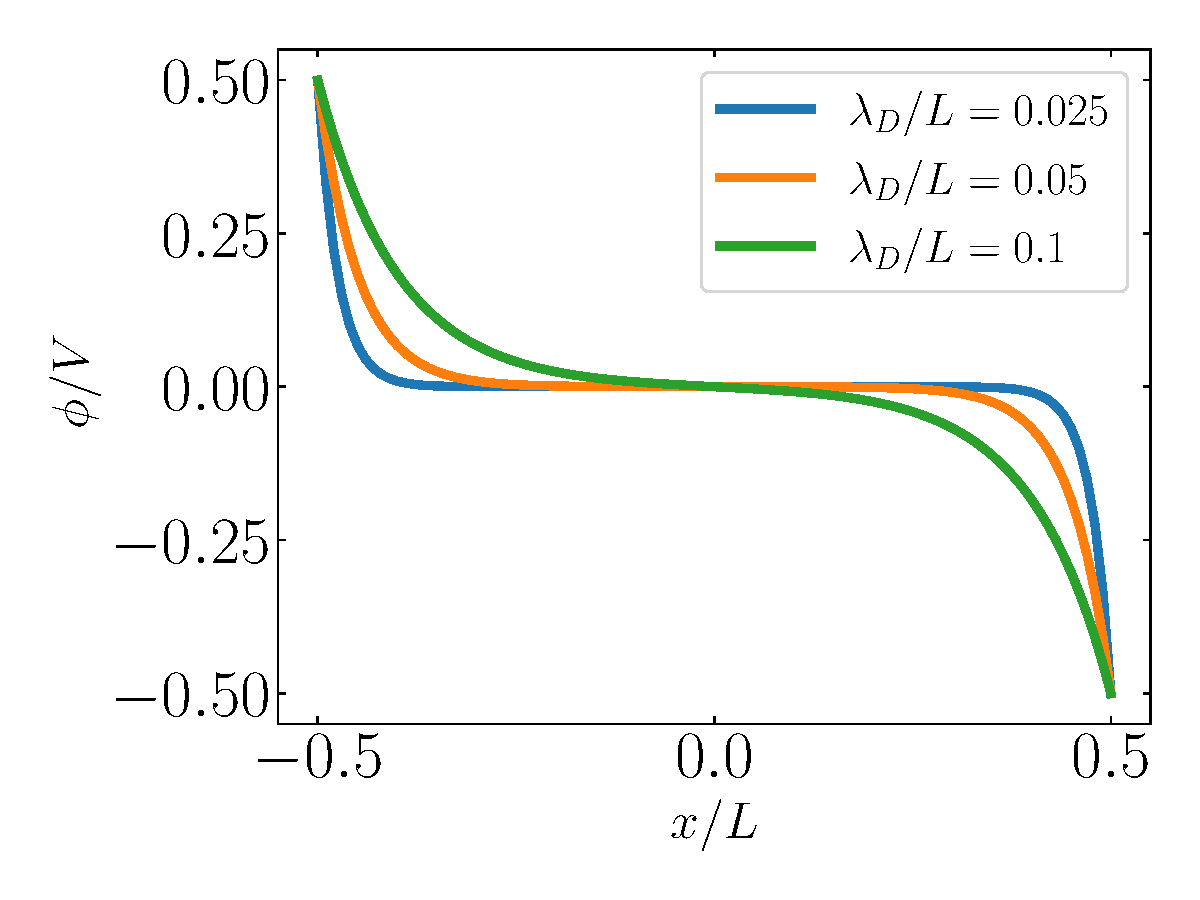
\includegraphics[width=\textwidth]{../../images/debye_phi.pdf}
        \caption{}
        \label{fig:debye_phi}
    \end{subfigure}
    \begin{subfigure}[b]{0.45\textwidth}
        \centering
        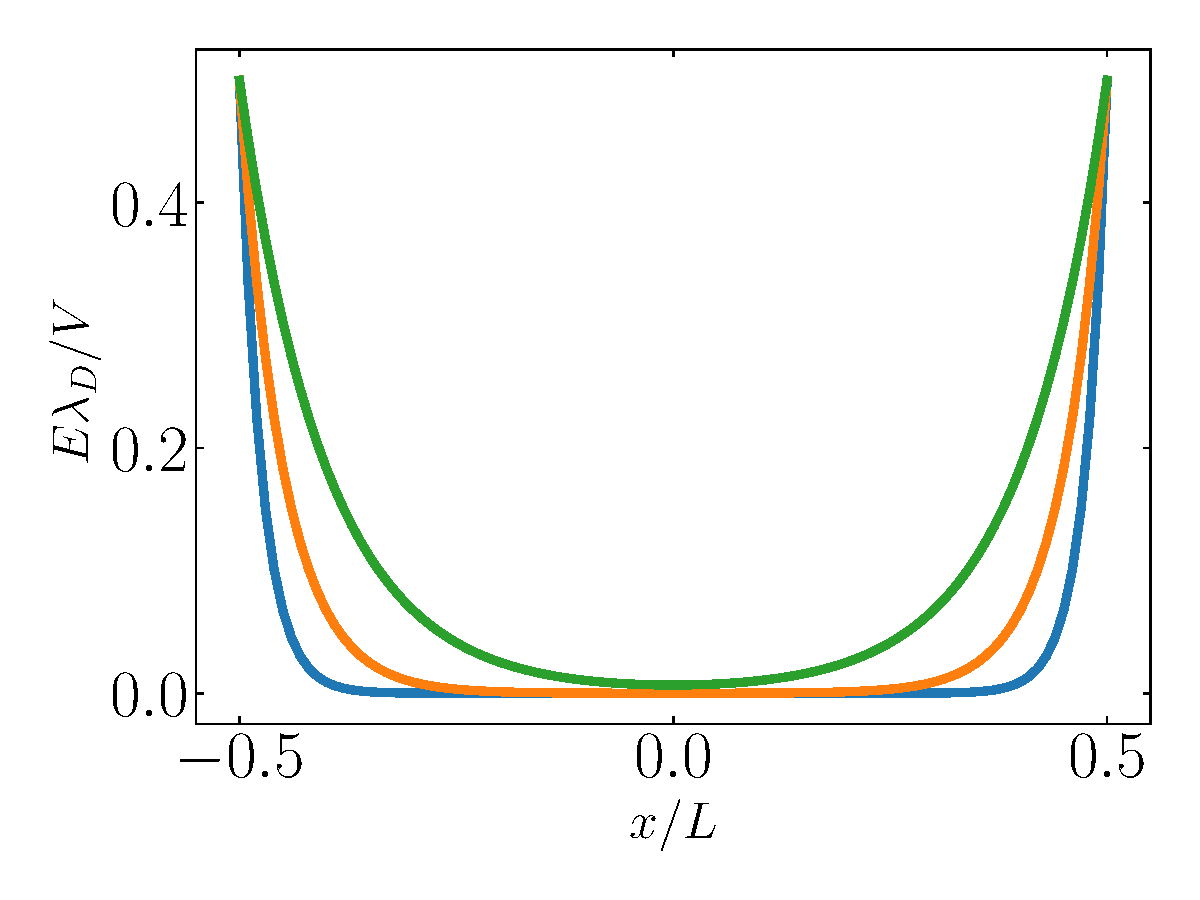
\includegraphics[width=\textwidth]{../../images/debye_elec.pdf}
        \caption{}
        \label{fig:debye_elec}
    \end{subfigure}
    \caption{Electric potential and field for various values of $\lambda_D/L$.}
    \label{fig:debye_phi_elec}
\end{figure}

We note that $\lambda_{De}$,  $w_{pe}$, and $v_{Te}$ are all related to each other as shown below
\begin{equation}
    \label{eq:debye_3vars}
    \lambda_{De} w_{pe} = \left ( \frac{\epsilon_0 k_B T_e}{n_{e0} e^2} \right )^{1/2} \left ( \frac{n_{e0} e^2}{m_e \epsilon_0} \right )^{1/2} = \left ( \frac{k_B T_e}{m_e} \right )^{1/2} = v_{Te}.
\end{equation}

%--------------------------------------------
\subsection{Plasma frequency}
%--------------------------------------------
At the end of \cref{sec:ep_waves} we assumed $w_{pe} < w$ in \cref{eq:ep_waves_pre_dispersion} to obtain a dispersion relation for electron-plasma waves. We now consider the cases $w_{pe} > w$ and $w_{pe} = w$ to better understand the role played by the plasma frequency $w_{pe}$.

We first consider the case of $w_{pe} > w$. Plugging in \cref{eq:ep_waves_efield_divergence} in \cref{eq:ep_waves_pre_dispersion} and using the definition of the electric potential, we have 
\begin{equation}
    \label{eq:plasma_freq_quartic}
    (w^2 - w_{pe}^2) \nabla^2 \phi_1 + \gamma_e v_{Te}^2 \nabla^4 \phi_1 = 0.
\end{equation}
We'll use the same setting as that for the derivation of the Debye length. The only difference is that the potential drop across the domain now oscillates with a frequency of $w$, that is $\phi_1(-L/2) - \phi_1(L/2) = V \exp (-iwt)$. Simplifying due to the one-dimensional domain and re-arranging, \cref{eq:plasma_freq_quartic} becomes
\begin{equation*}
     \frac{d^4 \phi_1}{dx^4} - \frac{w_{pe}^2 - w^2}{\gamma_e v_{Te}^2} \frac{d^2 \phi_1}{dx^2} = 0.
\end{equation*}
Using \cref{eq:debye_3vars} the above becomes
\begin{equation*}
    \frac{d^4 \phi_1}{dx^4} - \frac{1}{\gamma_e \lambda_{De}^2} \left ( 1 - \frac{w^2}{w_{pe}^2} \right ) \frac{d^2 \phi_1}{dx^2} = 0,
\end{equation*}
which we re-write as
\begin{equation*}
    \frac{d^4 \phi_1}{dx^4} - \frac{1}{\hat{\lambda}^2_{De}} \frac{d^2 \phi_1}{dx^2} = 0,
\end{equation*}
where 
\begin{equation*}
    \hat{\lambda}_{De}^2 = \gamma_e \lambda_{De}^2 \left ( 1 - \frac{w^2}{w_{pe}^2} \right )^{-1}.
\end{equation*}  
Integrating the fourth-order PDE above twice, we get
\begin{equation*}
    \frac{d^2 \phi_1}{dx^2} - \frac{1}{\hat{\lambda}^2_{De}} \phi_1 + C_1 x + C_2= 0
\end{equation*}
Since to obtain \cref{eq:ep_waves_pre_dispersion} we assumed $n_{e1} = \tilde{n}_{e1} \exp(-iwt)$, where $\tilde{n}_{e1} = \tilde{n}_{e1}(\xvec)$, we'll also assume $\phi_1 = \tilde{\phi}_1 \exp(-iwt)$, where $\tilde{\phi}_1 = \tilde{\phi}_1(\xvec)$. Plugging this into the ODE above we get
\begin{equation*}
     \left (\frac{d^2 \tilde{\phi}_1}{dx^2} - \frac{1}{\hat{\lambda}^2_{De}} \tilde{\phi}_1 \right ) + \left ( \frac{C_1 x + C_2}{\exp(-iwt)} \right )= 0
\end{equation*}
Note that the first term in parenthesis above does not depend on time, and thus the second term in parenthesis should not do so either. This can only be accomplished if we set $C_1 = C_2 = 0$. Thus we finally have
\begin{equation}
    \frac{d^2 \tilde{\phi}_1}{dx^2} - \frac{1}{\hat{\lambda}^2_{De}} \tilde{\phi}_1 = 0.
\end{equation}
The solution to the above that also conforms to the boundary conditions is ...

It is often important to know the plasma density at which the electron plasma frequency $w_{pe}$ equals the external frequency $w$. This density is referred to as the critical density $n_{cr}$. Equating the electron plasma frequency with the external frequency we get
\begin{equation*}
    \frac{n_{cr} e^2}{m_e \epsilon_0} = w^2,
\end{equation*}
which leads to
\begin{equation}
    \label{eq:plas_freq_crit_den}
    n_{cr} = \frac{m_e \epsilon_0 w^2}{e^2}
\end{equation}
The above can be re-written as
\begin{equation*}
    n_{cr} = \frac{m_e \epsilon_0 (2 \pi \nu)^2}{e^2} = \frac{4 \pi^2 m_e \epsilon_0 c^2}{e^2} \frac{1}{\lambda^2} = 1.115 \times 10^{27} \frac{1}{\lambda_{\mu m}^2},
\end{equation*}
where $\lambda_{\mu m}$ is in units of microns and $n_{cr}$ in units of \#/m\textsuperscript{3}.

%--------------------------------------------
\subsection{The coupling parameter}
%--------------------------------------------

Coulomb interactions are those which occur when two charge particles head towards each other. We can define two types of Coulomb interactions: strong and weak. Strong Coulomb interactions are those for which the particle's Coulomb potential energy is larger than its kinetic energy, and vice versa for weak Coulomb interactions. Thus, we can also define two types of plasma regimes:
\begin{itemize}
    \item Strongly-coupled plasmas: plasmas where the Coulomb interactions are mostly strong and thus drive the dynamics of its evolution. Coulomb interactions tend to be strong when the inter-particle distances are small, and thus this regime would be dominated by \textit{short-range} interactions. These plasmas are also described as exhibiting \textit{collisional} behavior, since a strong Coulomb interaction essentially means a collision has occurred.
    \item Weakly-coupled plasmas: plasmas where the Coulomb interactions are mostly weak, and as a result do not drive the dynamics of its evolution. The plasma dynamics are instead driven by \textit{long-range} effects caused by smooth electromagnetic fields that result from integrating a large number of particles. These plasmas are also described as exhibiting \textit{collective} behavior, since the long-range electromagnetic fields follow from the collective integration of many particles.
\end{itemize}

We describe an approximate Coulomb potential energy for particles in a plasma as
\begin{equation}
    U =  \frac{q_s^2}{4 \pi \epsilon_0 a_s}.
\end{equation}
The impact parameter that has been used above is $a_s$, the sphere radius. This provides a decent measure on the average spacing between particles in a plasma. Since the volume of a single particle is $1/n_s$, and if we assume that this volume is given by $4/3 \pi a_s^3$, then equating these two gives the expression for the sphere radius
\begin{equation}
    a_s = \left ( \frac{3}{4 \pi n_s} \right )^{1/3}.
\end{equation}
The thermal velocity of a particle is given by
\begin{equation}
    v_{T_s} = \sqrt{\frac{k_B T_s}{m_s}}
\end{equation}
A measure of the kinetic energy of a particle is given in terms of the thermal velocity as shown below
\begin{equation}
    K = m_s v_{T_s}^2 = k_B T_s
\end{equation}
The ratio of the particle's Coulomb potential energy and its kinetic energy is referred to as the coupling parameter $\Gamma_s$. That is 
\begin{equation}
    \Gamma_s = \frac{q_s^2}{4 \pi \epsilon_0 a_s k_B T_s}.
\end{equation}
$\Gamma_s > 1$ denotes a strongly coupled plasma, and $\Gamma_s < 1$ denotes a weakly coupled plasma. 

%--------------------------------------------
\subsection{The plasma parameter}
%--------------------------------------------
The standard plasma parameter $\Lambda_s$ is defined as
\begin{equation}
    \Lambda_s = \frac{4}{3} \pi \lambda_{Ds}^3 n_s.
\end{equation}

There is a one to one relationship between the coupling parameter and the standard plasma parameter. Simple algebra shows that 
\begin{equation}
    \Gamma_s = (1/3) \Lambda_s^{-2/3}.
\end{equation}
Thus, the coupling and plasma parameters are inversely proportional to each other. $\Lambda_s < 1$ implies strongly-coupled plasmas, and $\Lambda_s > 1$ weakly-coupled plasmas. Since $\Lambda_s$ represents the number of particles per Debye sphere, it is interesting to see that a large number of particles within such a sphere is needed to be in the weakly-coupled-plasma regime. However, this does not correspond to a plasma with large density, in fact, it corresponds to the opposite. The explicit $n_s$ term in the definition $\Lambda_s = (4/3) \pi \lambda^3_{Ds} n_s$ is dominated by the $n_s$ in the denominator of $\lambda_{Ds}$. In other words, low plasma densities lead to large Debye spheres, which in turn leads to many particles per Debye sphere, and hence a weakly-coupled plasma.

%--------------------------------------------
\subsection{Electron degeneracy}
%--------------------------------------------

\begin{itemize}
    \item DeBroglie wavelength
    \begin{equation}
        \lambda_{Bs} = \dfrac{h}{\sqrt{2 \pi} m_s v_{Ts}}
    \end{equation}
    \item Quantum plasma parameter
    \begin{equation}
        \chi_s = \frac{4}{3} \pi \lambda_{Bs}^3 n_s
    \end{equation}
    
    \item Fermi energy:
    \begin{equation}
        E_{fs} = \frac{\hbar^2}{2m_s} \left ( 3 \pi^2 n_s \right)^{2/3}
    \end{equation}

    \item The Fermi energy can be used to define the Fermi temperature $T_{fs}$, Fermi velocity $v_{fs}$, Fermi momentum $p_{fs}$, and Fermi wave vector $k_{fs}$
    \begin{equation}
        E_{fs} = k_B T_{fs} = \frac{1}{2} m_s v_{fs}^2  = \frac{p_{fs}^2}{2m_s} = \frac{\left ( \hbar k_{fs} \right ) ^2}{2m_s}
    \end{equation}

    \item Degeneracy parameter:
    \begin{equation}
        \Theta_s = \frac{k_B T_s}{E_{fs}} = \left( \frac{2^{10} \pi}{3^4} \right)^{1/3} \chi_s^{-2/3}.
    \end{equation}
\end{itemize}

%########################################################################
\chapter{Collisions}
%########################################################################
%------------------------------------------------------------------------
\section{Cross section}
%------------------------------------------------------------------------
%--------------------------------------------
\subsection{General definition}
%--------------------------------------------
Two particles traveling towards each other can undergo an interaction. Types of interactions include Coulomb collisions between two charged particles, fusion reactions between ions, and photon-matter phenomena such as Compton scattering, the photoelectric effect, and pair production.

\begin{figure}[ht]
    \centering
    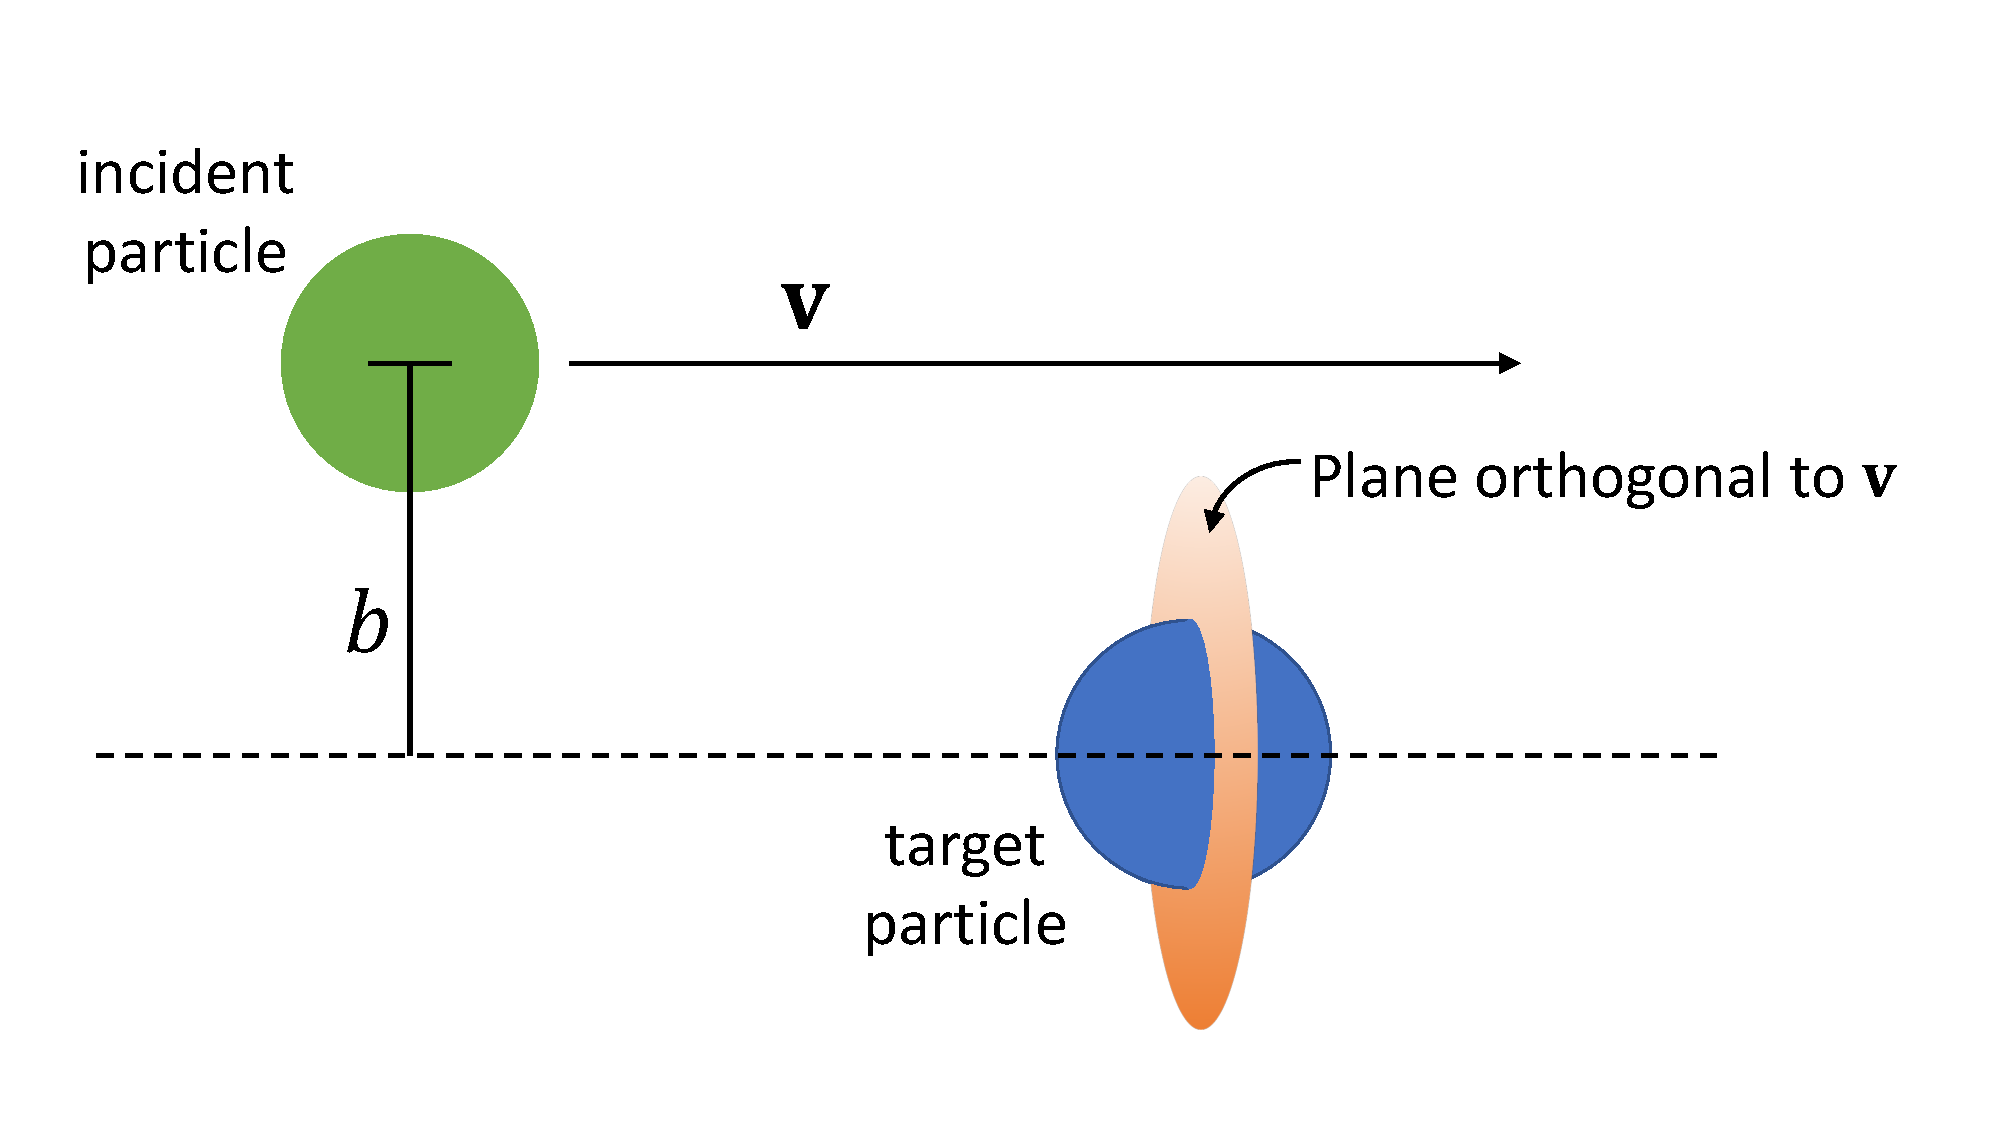
\includegraphics[width=10cm]{../../images/cross_section.pdf}
    \caption{Interaction of incident and target particles.}
    \label{fig:cross_many_particles}
\end{figure}
To define the cross section, we'll consider $I$ incident particles heading towards $J$ stationary target particles (see \cref{fig:cross_many_particles}). Not all of the incident particles will interact with the target particles, some will instead continue to travel in a uniform trajectory. The number of incident particles that do interact with the target particles is labeled as $N$. The cross section $\sigma$ is then a constant of proportionality defined by the following equation
\begin{equation}
    \label{eq:cross_def}
    N = \sigma I n_A.
\end{equation}
In the above, $n_A$ is the areal number density, that is, $n_A = J / A = n \Delta x$, where $n$ is the volume number density.

%--------------------------------------------
\subsection{Differential cross section}
%--------------------------------------------
\begin{figure}[ht]
    \centering
    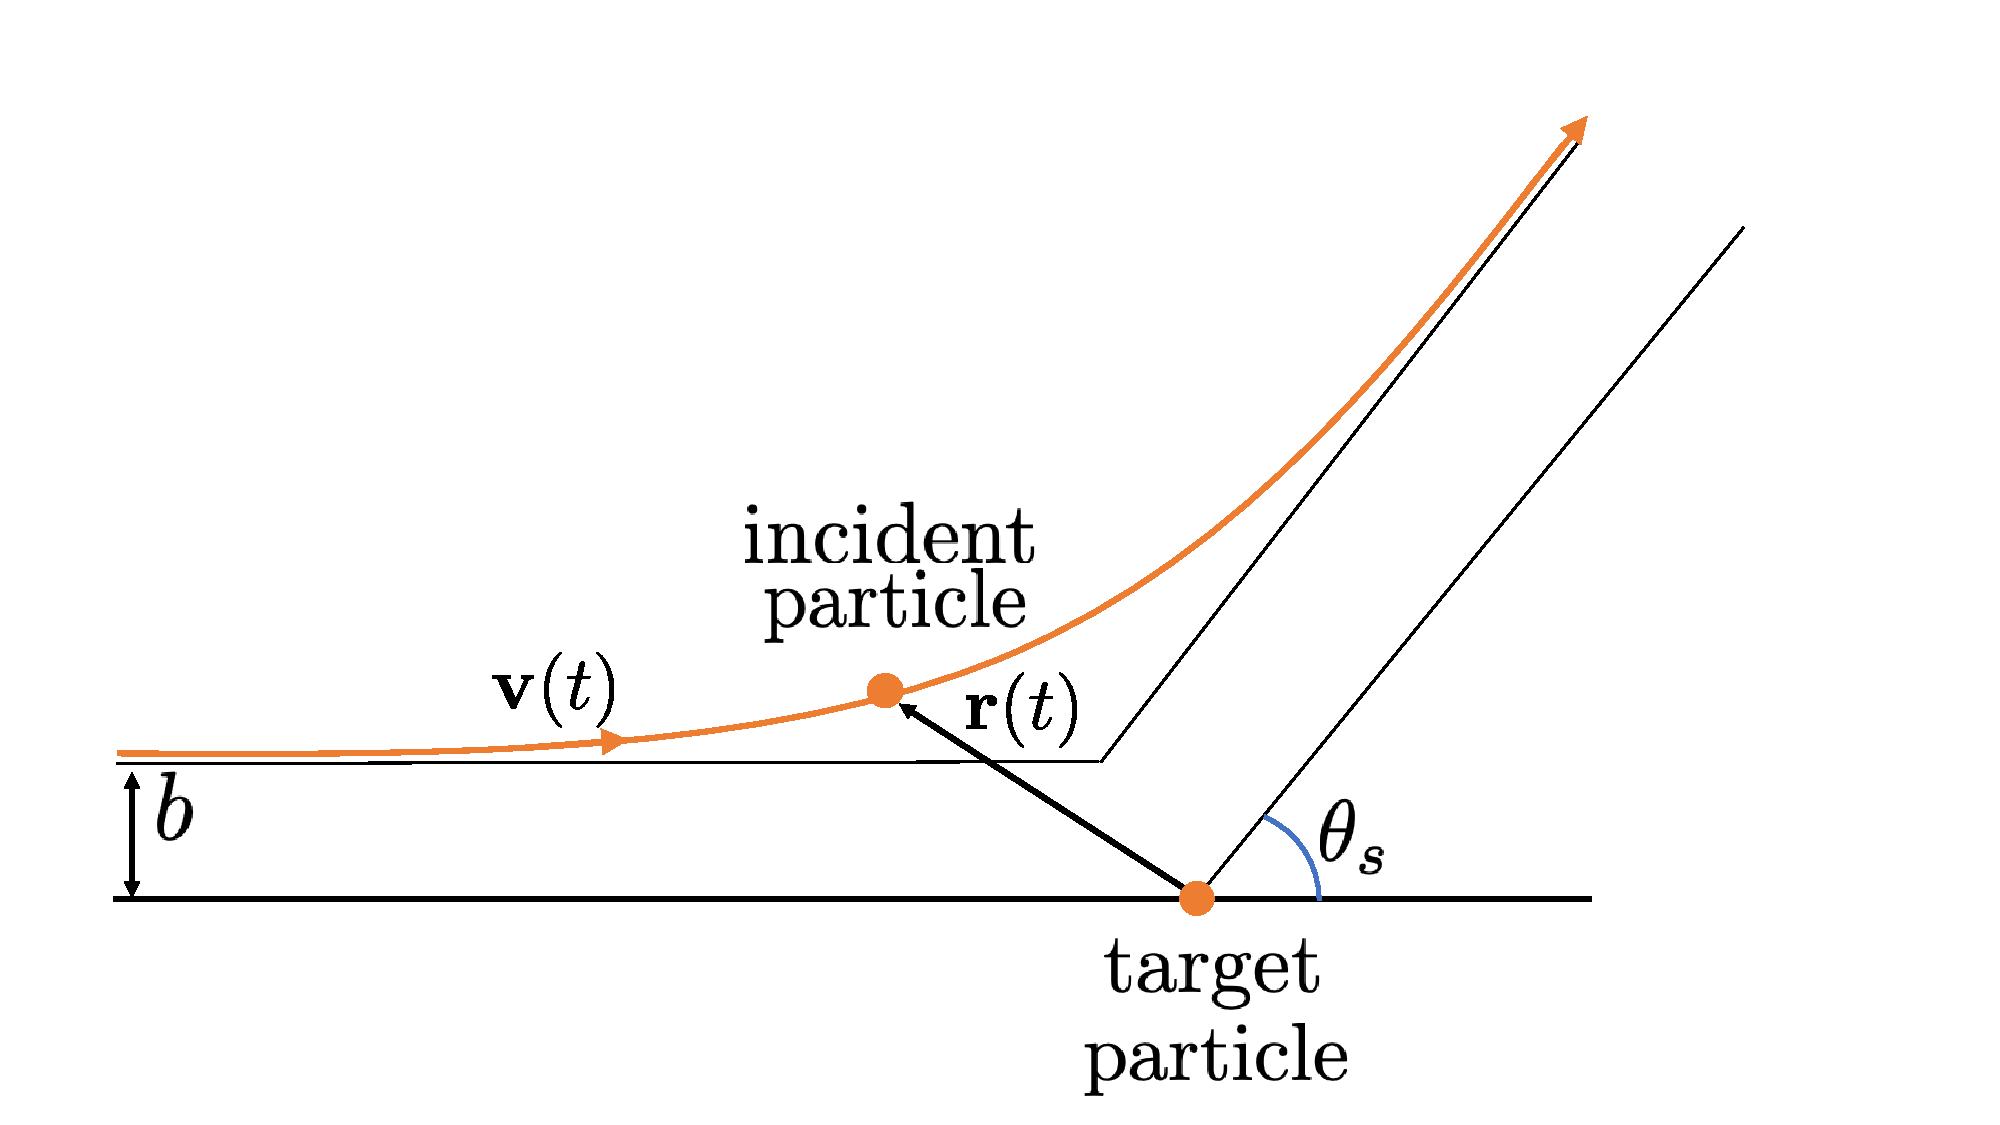
\includegraphics[width=10cm]{../../images/scattering.pdf}
    \caption{Depiction of particle scattering.}
    \label{fig:scattering}
\end{figure}

Consider the scattering of two particles: an incident and a target particle. If we fix the reference frame to follow the target particle, then the scattering can be depicted as shown in \cref{fig:scattering}. The displacement parameter is labelled as $b$, and the scattering angle as $\theta_s$. For three dimensional scattering, the encounter is as shown in \cref{fig:scattering_3d}. Not that in that figure the incident particle starts within the $x-z$ plane, and after scattering the particle is confined to a plane that is tilted an angle $\phi_s$ from the $x-z$ plane.

\begin{figure}[ht]
    \centering
    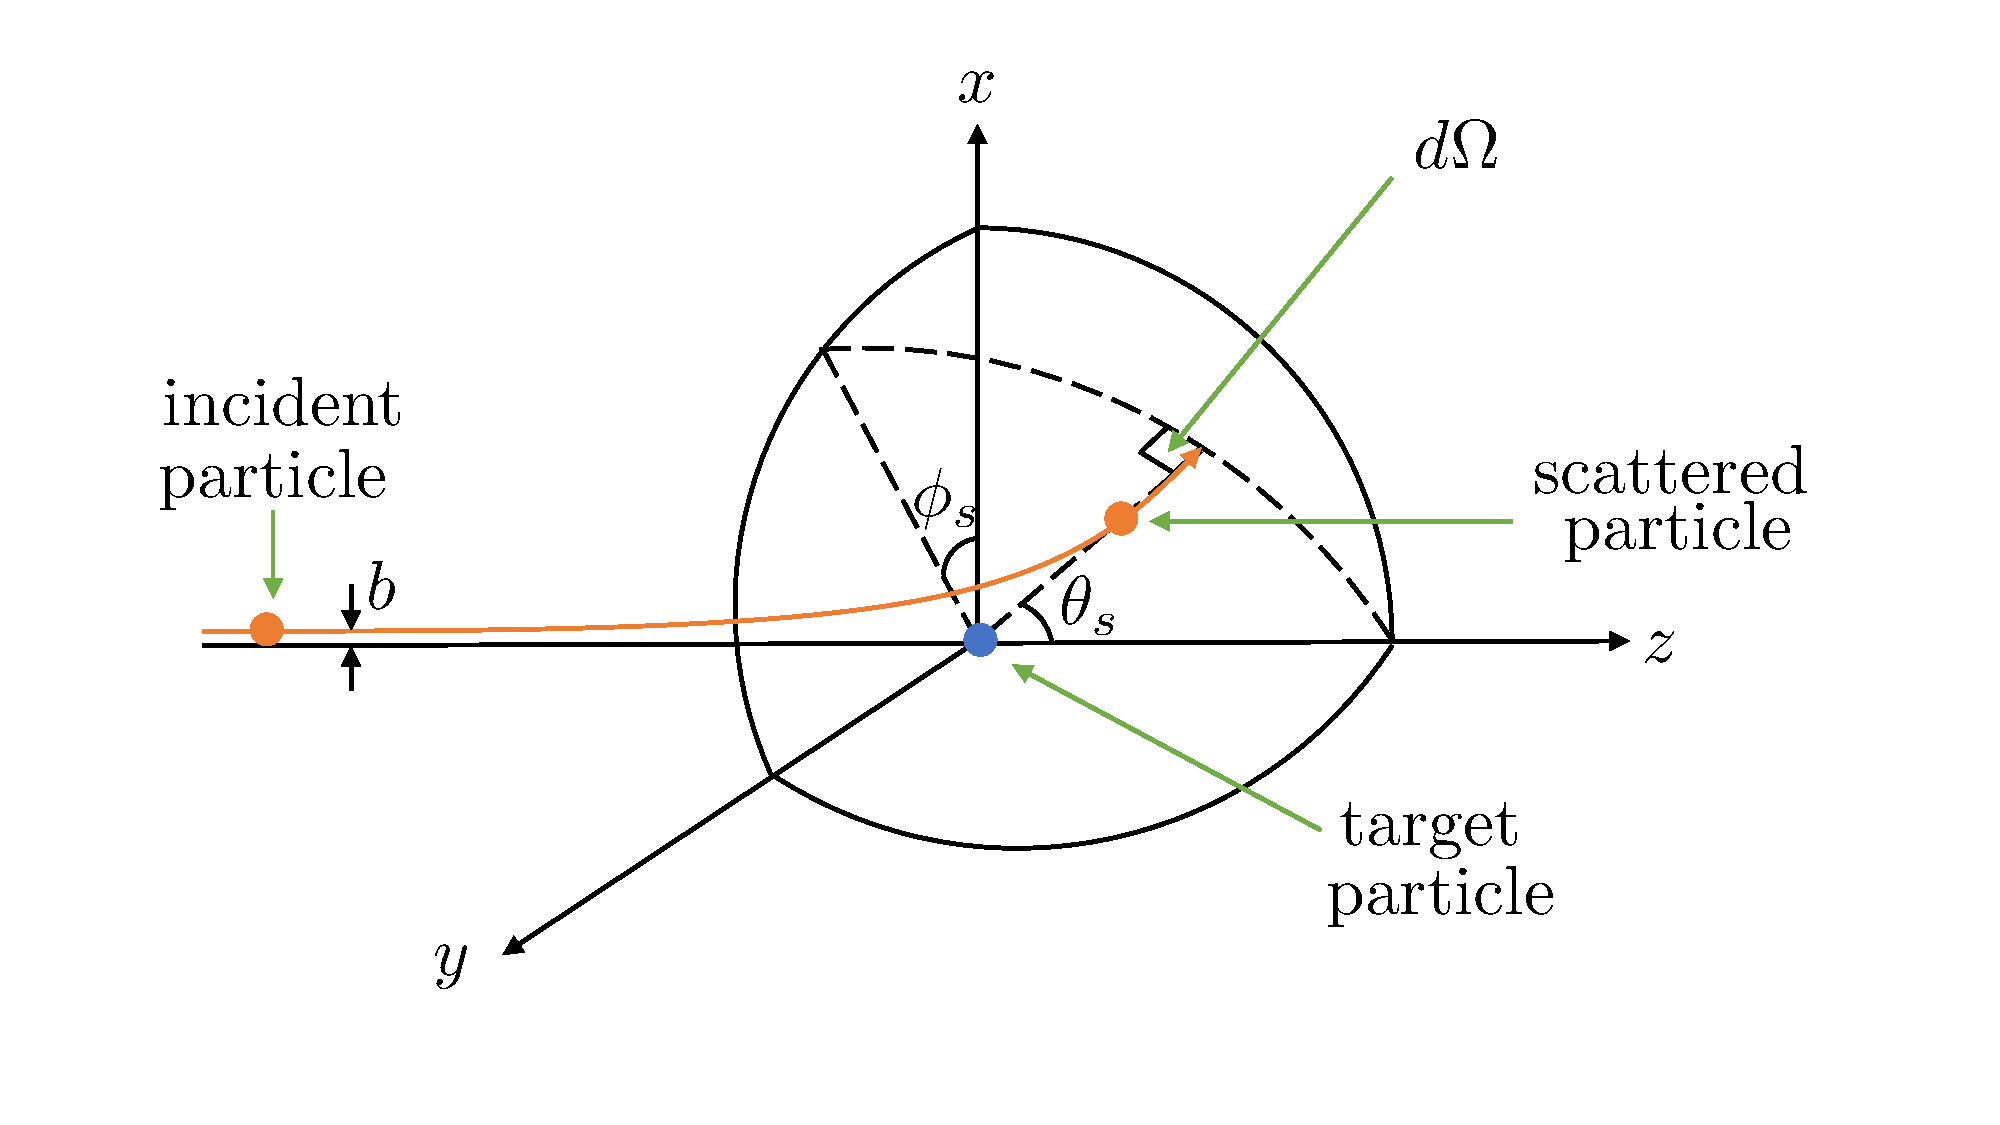
\includegraphics[width=10cm]{../../images/scattering_3d.pdf}
    \caption{Depiction of particle scattering in 3D.}
    \label{fig:scattering_3d}
\end{figure}

From the entire set of incident particles $N$ that interact with the target particles, one can define an infinitesimal subset $N_{\theta,\phi} d\Omega$ as the number of particles scattered into an infinitesimal solid angle $d\Omega = \sin \theta_s d\theta_s d\phi_s$, as shown in \cref{fig:scattering_3d}. We note that $N_{\theta,\phi} = N_{\theta,\phi} (\theta_s, \phi_s)$. We introduce the differential cross section
\begin{equation}
    \frac{d\sigma_{\theta,\phi}}{d\Omega} = \frac{d\sigma_{\theta,\phi}}{d\Omega}(\theta_s,\phi_s),
\end{equation}
which is defined by the following expression in an analogous manner to \cref{eq:cross_def},
\begin{equation}
    \label{eq:cross_def_diff}
    N_{\theta, \phi} d\Omega = \left ( \frac{d\sigma_{\theta,\phi}}{d\Omega} d\Omega \right ) I n_A.
\end{equation}
It is best to not think of it as a derivative (what does a derivative with respect to solid angle mean?) and instead to simply think of it as a function that depends on $\theta_s$ and $\phi_s$. Integrating over all $\theta_s$ and $\phi_s$, i.e.
\begin{equation*}
    \int_{\theta_s = 0}^\pi \int_{\phi_s = 0}^{2\pi} N_{\theta, \phi} d\Omega = \int_{\theta_s = 0}^\pi \int_{\phi_s = 0}^{2\pi} \frac{d\sigma_{\theta,\phi}}{d\Omega}  d\Omega I n_A
\end{equation*}
gives \cref{eq:cross_def}.

\begin{figure}[ht]
    \centering
    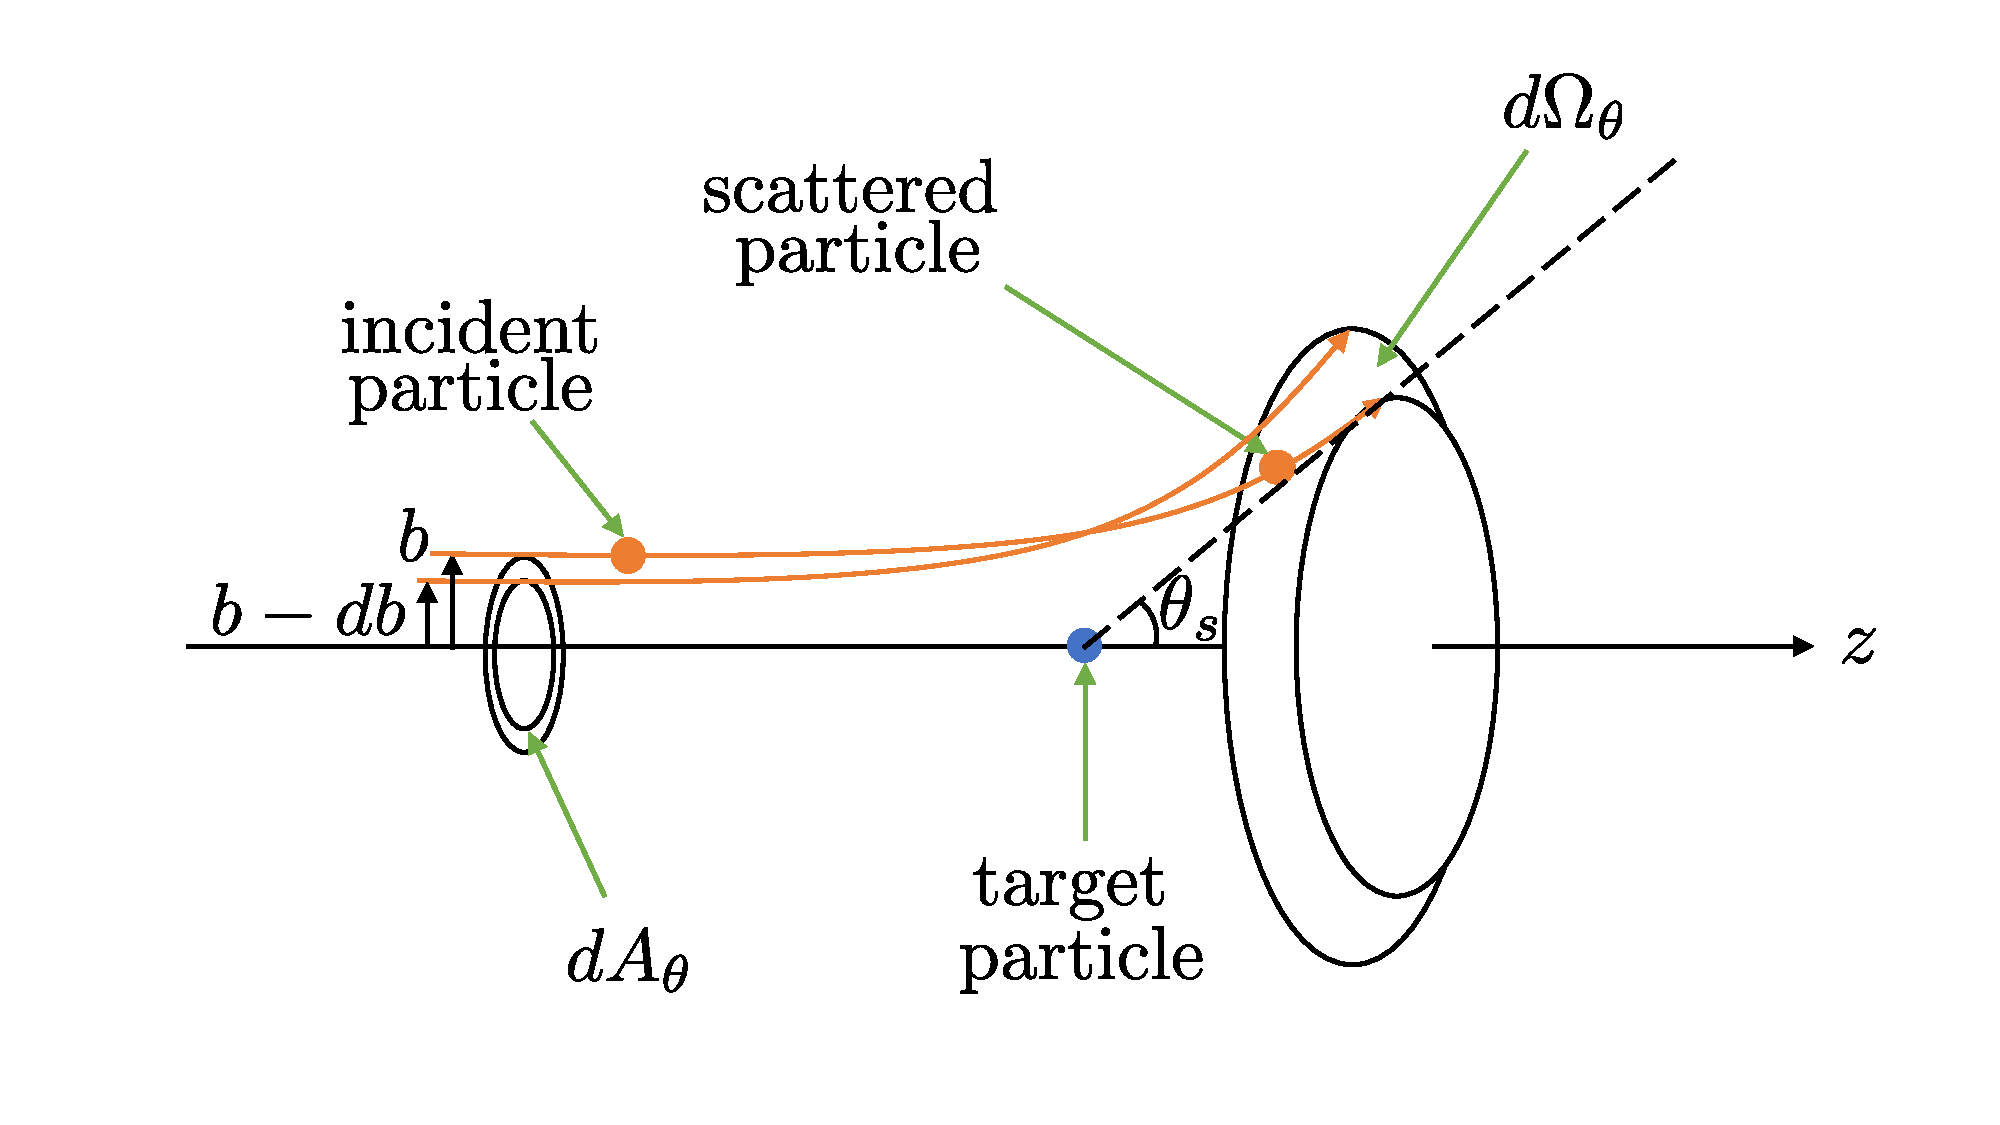
\includegraphics[width=10cm]{../../images/scattering_axi.pdf}
    \caption{Depiction of particle scattering in for axi-symmetric interactions.}
    \label{fig:scattering_axi}
\end{figure}
For various cases the scattering is axi-symmetric, that is, it is independent of $\phi_s$. Thus
\begin{equation*}
    N_{\theta, \phi} \to N_\theta \qquad \frac{d\sigma_{\theta,\phi}}{d\Omega} \to \frac{d\sigma_\theta}{d\Omega},
\end{equation*}
where 
\begin{equation*}
    N_\theta = N_\theta (\theta_s),
\end{equation*}
and
\begin{equation*}
    \frac{d\sigma_\theta}{d\Omega} = \frac{d\sigma_\theta}{d\Omega} (\theta_s).
\end{equation*}
Integrating \cref{eq:cross_def_diff} from $\phi_s = 0$ to $\phi_s = 2\pi$ gives
\begin{equation}
    \label{eq:cross_def_diff_axi}
    N_\theta d\Omega_\theta = \frac{d\sigma_\theta}{d\Omega} d\Omega_\theta I n_A,
\end{equation}
where $d \Omega_\theta = 2\pi \sin \theta_s d\theta_s$. $N_\theta d\Omega_\theta$ thus represents the number of particles that are scattered into the infinitesimal band $d\Omega_\theta$ on a sphere, where $d\Omega_\theta$ is defined by scattering angle $\theta_s$ (see \cref{fig:scattering_axi}). We will note that there is a one-to-one correspondence between the impact parameter $b$ and the scattering angle $\theta_s$, that is, $b = b(\theta_s)$. In other words, any incident particle scattered out through the infinitesimal band $d\Omega_\theta$ would have approached the target-particle through the infinitesimal ring $dA_\theta$ that corresponds to $d\Omega_\theta$. Since there are many target particles, there are many $dA_\theta$'s that correspond to the same $d\Omega_\theta$. Thus, the total number of particles scattered through $d\Omega_\theta$ is given by all the incident particles that cross through the $dA_\theta$'s of all the target particles.

The number of incident particles crossing all the infinitesimal rings $dA_\theta$ is equal to the total number of incident particles $I$ times the probability $P$ that any single incident particle will cross one of those rings. Thus, we can write
\begin{equation*}
    N_\theta d\Omega_\theta = I P.
\end{equation*}
The probability that an incident particle will cross one of those rings is simply the ratio of the surface area covered by all the rings in a section of the target material to the total area of that section. The surface area covered by all the rings in a section of area $S$ is given by $(n_A S) dA_\theta$. Thus, $P = n_A dA_\theta$ and 
\begin{equation*}
    N_\theta d\Omega_\theta = I n_A dA_\theta.
\end{equation*}
We now introduce the differential 
\begin{equation}
    \label{eq:cross_impact_differential}
    db = \frac{db}{d\theta_s} d\theta_s.
\end{equation}
We note that by definition $d\theta_s$ is positive but $db$ can be either positive or negative depending on the sign of $db/d\theta_s$. The infinitesimal area $dA_\theta$ is then given by 
\begin{equation}
    \label{eq:cross_impact_area}
    dA_\theta= 2\pi b |db| = 2 \pi b \left | \frac{db}{d\theta_s} \right | d \theta_s.
\end{equation}
Thus, 
\begin{equation*}
    N_\theta d\Omega_\theta = n_A I 2 \pi b \left | \frac{db}{d\theta_s} \right | d \theta_s.
\end{equation*}
Using \cref{eq:cross_def_diff_axi} in the above, we get
\begin{equation*}
    \frac{d\sigma_\theta}{d\Omega} d\Omega_\theta I n_A = I n_A 2 \pi b \left | \frac{db}{d\theta_s} \right | d \theta_s, 
\end{equation*}
or 
\begin{equation}
    \label{eq:cross_diff_impact_axi}
    \frac{d\sigma_\theta}{d\Omega} = \frac{b}{\sin \theta_s} \left | \frac{db}{d\theta_s} \right |.
\end{equation}

%--------------------------------------------
\subsection{Mean free path \& collision frequency}
%--------------------------------------------
The mean free path can be expressed in terms of the cross section as
\begin{equation}
    \lambda_m = \frac{1}{n_1 \sigma}.
\end{equation}
Given the particle's speed $v$, on can also define the collision time as follows
\begin{equation}
    \tau_m = \frac{\lambda_m}{v} = \frac{1}{n_1 \sigma v}.
\end{equation}
Finally, the collision frequency is simply the inverse of the collision time, that is
\begin{equation}
    \nu_{m} = \frac{1}{\tau_m} = n_1 \sigma v.
\end{equation}

%------------------------------------------------------------------------
\section{Coulomb collisions}
%------------------------------------------------------------------------

%--------------------------------------------
\subsection{Particle equations}
%--------------------------------------------
\label{sec:coulomb_particle_equations}
Consider two particles, with positions $\rvec_1=\rvec_1(t)$ and $\rvec_2=\rvec_2(t)$, velocities $\vvec_1=\vvec_1(t)$ and $\vvec_2=\vvec_2(t)$, charges $q_1$ and $q_2$, and masses $m_1$ and $m_2$, respectively. Their positions and velocities are governed by the following equations 
\begin{equation}
    \label{eq:coul_particle_1_pos}
    \frac{d \rvec_1}{dt} = \vvec_1,
\end{equation}
\begin{equation}
    \label{eq:coul_particle_2_pos}
    \frac{d \rvec_2}{dt} = \vvec_2,
\end{equation}
\begin{equation}
    \label{eq:coul_particle_1_vel}
    m_1 \frac{d\vvec_1}{dt} = -\frac{q_1 q_2}{4 \pi \epsilon} \frac{\rvec_2 - \rvec_1}{\left | \rvec_2 - \rvec_1 \right |^3},
\end{equation}
\begin{equation}
    \label{eq:coul_particle_2_vel}
    m_2 \frac{d\vvec_2}{dt} = -\frac{q_1 q_2}{4 \pi \epsilon} \frac{\rvec_1 - \rvec_2}{\left | \rvec_1 - \rvec_2 \right |^3}.
\end{equation}
We note that the above system consists of twelve equations for twelve unknowns. We now introduce the center-of-mass position $\Rvec = \Rvec(t)$, the center-of-mass velocity $\Vvec = \Vvec(t)$, the shifted position $\rvec = \rvec(t)$ and the shifted velocity $\vvec = \vvec(t)$ as follows
\begin{equation*}
    \Rvec = \frac{m_1 \rvec_1 + m_2 \rvec_2}{m_1 + m_2} \qquad \rvec = \rvec_1 - \rvec_2,
\end{equation*}
\begin{equation*}
    \Vvec = \frac{m_1 \vvec_1 + m_2 \vvec_2}{m_1 + m_2} \qquad \vvec = \vvec_1 - \vvec_2
\end{equation*}
Thus, in terms of these new four variables, the particle equations can be written as
\begin{equation}
    \frac{d \Rvec}{dt} = \Vvec,
\end{equation}
\begin{equation}
    \frac{d \Vvec}{dt} = 0 ,
\end{equation}
\begin{equation}
    \label{eq:particle_pos}
    \frac{d \rvec}{dt} = \vvec,
\end{equation}
\begin{equation}
    \label{eq:coul_particle_vel}
    \frac{d \vvec}{dt} = \frac{q_1 q_2}{4\pi \epsilon_0 m_r} \frac{\rvec}{r^3},
\end{equation}
where the reduced mass $m_r$ is given by
\begin{equation}
    \label{eq:coul_reduced_mass}
    \frac{1}{m_r} = \frac{1}{m_1} + \frac{1}{m_2}.
\end{equation}
The first two equations above give the trivial solution $\Vvec = $ constant and $\Rvec$ = $\Rvec(0) + \Vvec t$. Thus, we have reduced the problem from twelve unknowns to six unknowns, namely $\rvec$ and $\vvec$.

%--------------------------------------------
\subsection{Conservation of energy and momentum}
%--------------------------------------------
Dotting \cref{eq:coul_particle_vel} by $\vvec$ gives 
\begin{align*}
    \vvec \cdot \frac{d \vvec}{dt} &= \frac{q_1 q_2}{4 \pi \epsilon_0 m_r} \vvec \cdot \frac{\rvec}{r^3} \nonumber \\
    &= \frac{q_1 q_2}{4 \pi \epsilon_0 m_r} \frac{d\rvec}{dt} \cdot \frac{\rvec}{r^3} \nonumber \\
    &= \frac{q_1 q_2}{4 \pi \epsilon_0 m_r} \frac{1}{2} \frac{dr^2}{dt} \frac{1}{r^3} \nonumber \\
    &= \frac{q_1 q_2}{4 \pi \epsilon_0 m_r} \frac{1}{r^2} \frac{dr}{dt} \nonumber \\
    &= -\frac{q_1 q_2}{4 \pi \epsilon_0 m_r} \frac{d}{dt} \left ( \frac{1}{r} \right ).
\end{align*} 
For the left hand side above we have
\begin{equation*}
    \vvec \cdot \frac{d \vvec}{dt} = \frac{1}{2} \frac{d v^2}{dt},
\end{equation*}
and thus we obtain the following expression for conservation of energy
\begin{equation*}
    \frac{d}{dt} \left ( \frac{1}{2} m_r v^2 + \frac{q_1 q_2}{4 \pi \epsilon_0} \frac{1}{r} \right ) = 0.
\end{equation*}

Crossing \cref{eq:coul_particle_vel} by $\rvec$ gives
\begin{equation*}
    \rvec \times \frac{d \vvec}{dt} = \frac{q_1 q_2}{4 \pi \epsilon_0 m_r} \frac{\rvec \times \rvec}{r^3} = 0,
\end{equation*}
and thus
\begin{equation*}
    \frac{d}{dt} \left [ m_r \left ( \rvec \times \vvec \right ) \right ] = 0.
\end{equation*}
That is, angular momentum is conserved. A consequence of this is that the vector $\rvec \times \vvec$ is always pointing in the same direction. Thus, if $\rvec(0)$ and $\vvec(0)$ form a plane, then $\rvec(t)$ and $\vvec(t)$ need to reside within that same plane for all times $t$ so that $\rvec(t) \times \vvec(t)$ points in the same direction as $\rvec(0) \times \vvec(0)$. Therefore, the evolution of the position and velocity are confined to a plane and the problem can be reduced from six unknowns to four unknowns. This planar encounter is depicted in \cref{fig:coulomb_scattering}.
\begin{figure}[ht]
    \centering
    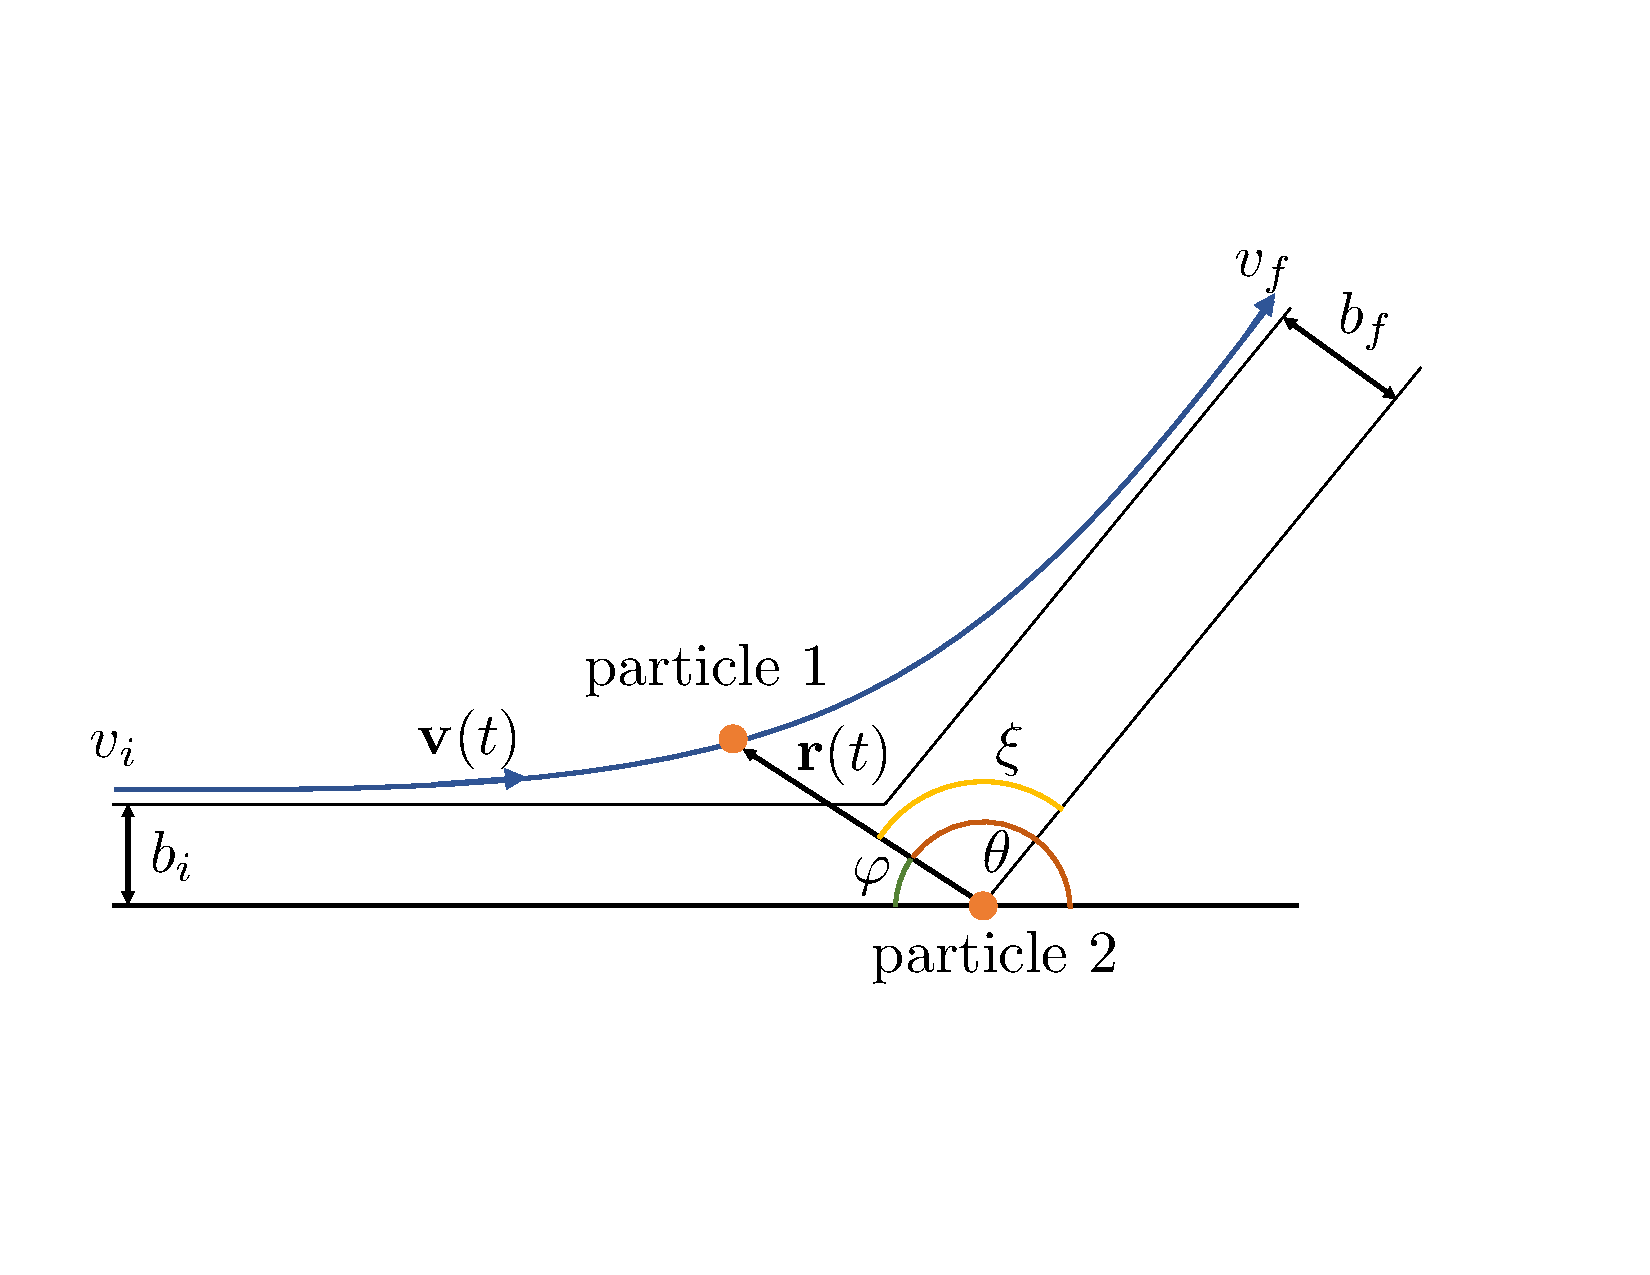
\includegraphics[width=10cm]{../../images/coulomb_scattering.pdf}
    \caption{Depiction of Coulomb scattering.}
    \label{fig:coulomb_scattering}
\end{figure}

If we refer to the plane shown in \cref{fig:coulomb_scattering} as the $x-y$ plane, then one can tell that the angular-momentum vector points in the negative $z$ direction. We will denote the magnitude of the conserved angular momentum by $L$, and thus we can write
\begin{equation}
    \label{eq:coul_cons_angular_momentum}
    m_r \left (\rvec \times \vvec \right ) = -L \hat{\zvec}.
\end{equation}

A consequence of both conservation of energy and momentum is as follows. Consider the two limiting states of particle 1---the initial state $v_i$, $b_i$ and the final state $v_f$, $b_f$. Assuming the potential energy is very low at sufficiently early and late times, conservation of energy gives
\begin{equation}
    \frac{1}{2} m_r v_i^2 = \frac{1}{2} m_r v_f^2,
\end{equation}
that is, $v_i=v_f$ (note that for other scattering processes, e.g.\@ Compton scattering, this is not necessarily the case). For the angular momentum of the initial state we have
\begin{multline}
    \label{eq:coul_cons_angular_momentum_derv1}
    m_r \left ( \rvec_i \times \vvec_i \right ) = m_r \sin(-\theta_i) r_i v_i \hat{\zvec} = - m_r \sin(\theta_i) r_i v_i \hat{\zvec} = - m_r \sin(\pi - \varphi_i) r_i v_i \hat{\zvec} \\
    = - m_r \sin(\varphi_i) r_i v_i \hat{\zvec} = -m_r b_i v_i \hat{\zvec}
\end{multline}
Similarly, for the angular momentum of the final state we have
\begin{equation}
    m_r \left ( \rvec_f \times \vvec_f \right ) = m_r \sin(-\xi_f) r_f v_f  \hat{\zvec} = - m_r \sin(\xi_f) r_f v_f \hat{\zvec} = - m_r b_f v_f \hat{\zvec}.
\end{equation}
Equating the last two relationships gives $m_r b_i v_i = m_r b_f v_f$. Since $v_i = v_f$, we finally have $b_i = b_f = b$. Using \cref{eq:coul_cons_angular_momentum} in \cref{eq:coul_cons_angular_momentum_derv1}, we can also write
\begin{equation}
    \label{eq:coul_cons_angular_momentum_mag}
    L = m_r b v_i.
\end{equation}

%--------------------------------------------
\subsection{Polar coordinates}
%--------------------------------------------
\begin{figure}[ht]
    \centering
    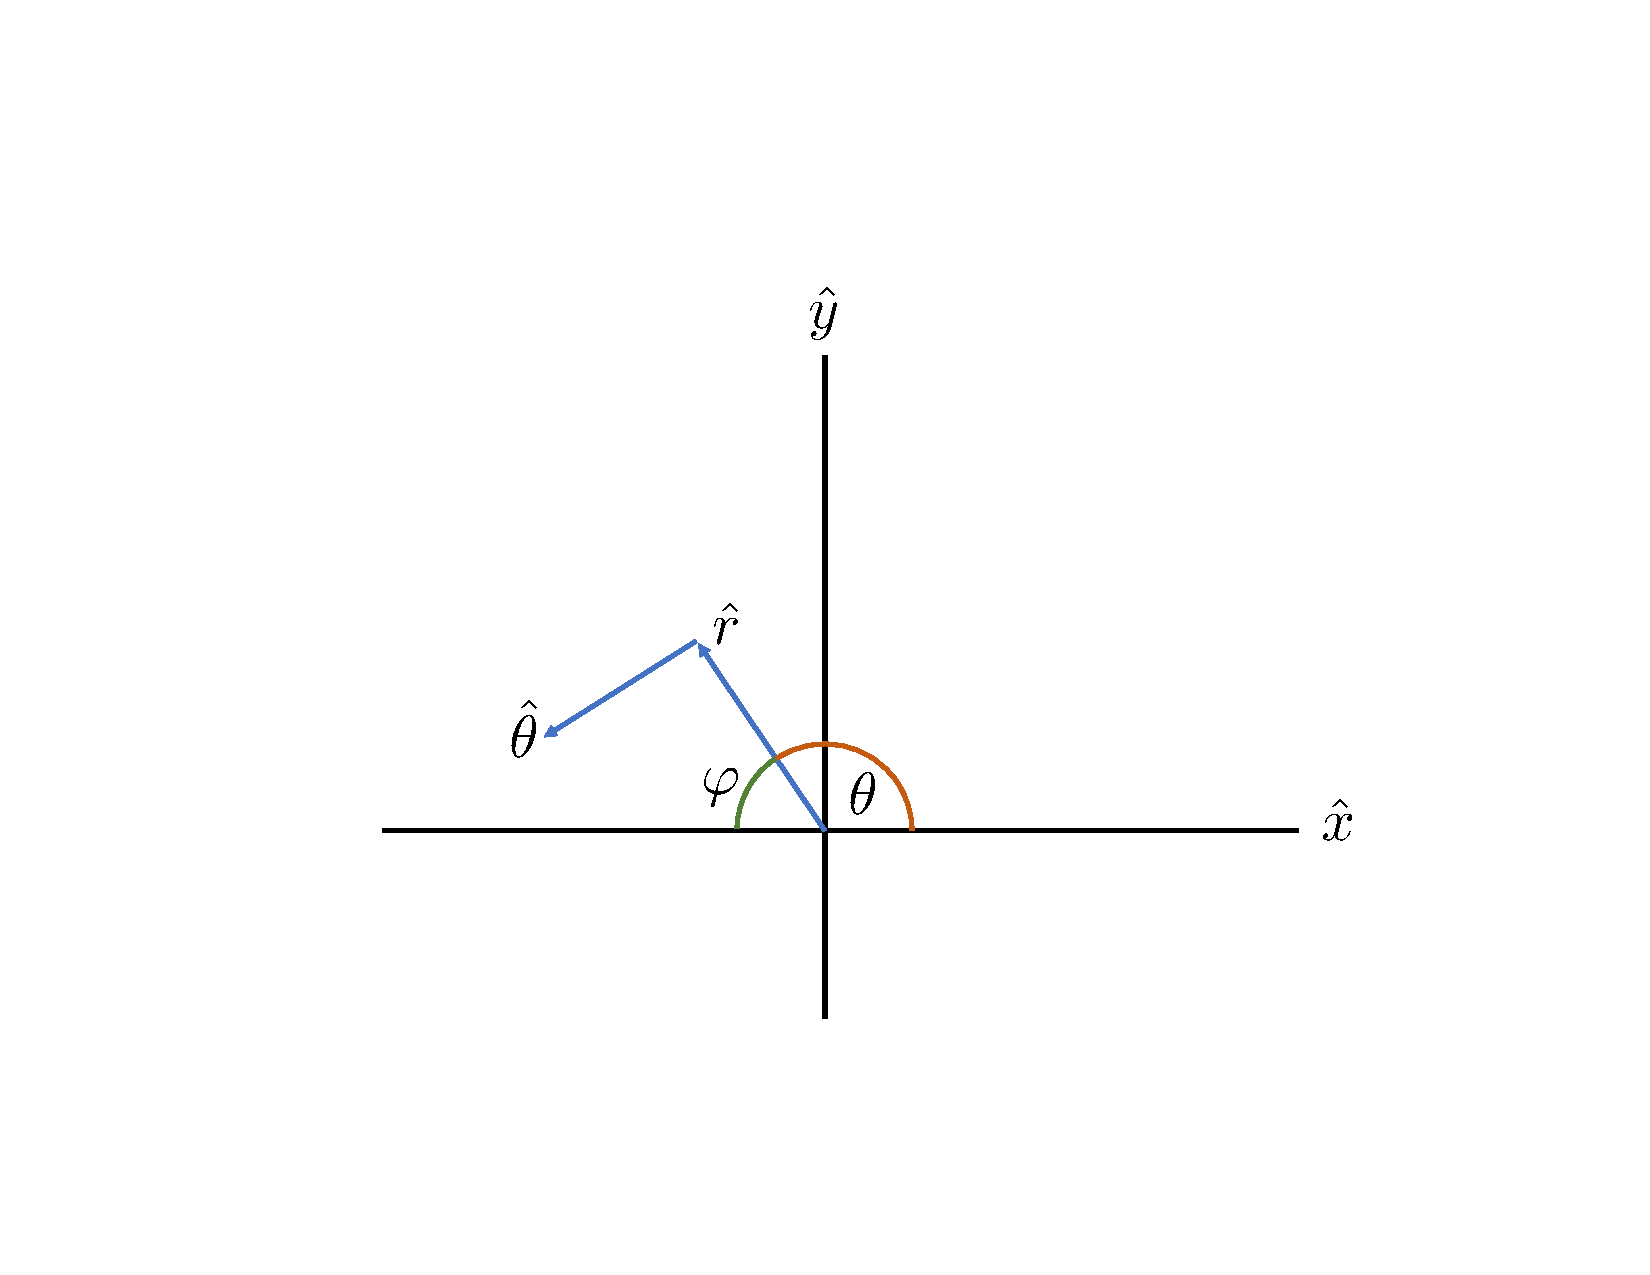
\includegraphics[width=10cm]{../../images/polar_coordinates.pdf}
    \caption{Polar coordinates in plane of interaction.}
    \label{fig:polar_coordinates}
\end{figure}

Using polar coordinates, as shown in \cref{fig:polar_coordinates}, we get
\begin{equation*}
    r_x = r \cos \theta = r \cos ( \pi - \varphi ) = -r \cos \varphi,
\end{equation*}
\begin{equation*}
    r_y = r \sin \theta = r \sin ( \pi - \varphi ) = r \sin \varphi.
\end{equation*}

Also, since $\rvec = r \hat{\rvec}$, we have
\begin{align*}
    \vvec = &\frac{d \rvec}{dt} = \frac{dr}{dt} \hat{\rvec} + r \frac{d\hat{\rvec}}{dt} \nonumber \\
    &= \frac{d r}{dt} \hat{\rvec} + r \frac{d\hat{\rvec}}{d\theta} \frac{d\theta}{dt} \nonumber \\
    &= \frac{dr}{dt} \hat{\rvec} + r \frac{d \theta}{dt} \hat{\bm{\theta}},
\end{align*}
and
\begin{align*}
    \frac{d \vvec}{dt} &= \frac{d^2r}{dt^2} \hat{\rvec} + \frac{dr}{dt} \frac{d\hat{\rvec}}{dt} + \frac{d}{dt} \left ( r \frac{d\theta}{dt} \right ) \hat{\bm{\theta}} + r \frac{d \theta}{dt} \frac{d \hat{\bm{\theta}}}{dt} \nonumber \\
    &= \frac{d^2 r}{dt^2} \hat{\rvec} + \frac{dr}{dt} \frac{d\hat{\rvec}}{d\theta} \frac{d\theta}{dt} + \frac{d}{dt} \left ( r \frac{d\theta}{dt} \right ) \hat{\bm{\theta}} + r \frac{d \theta}{dt} \frac{d \hat{\bm{\theta}}}{d\theta} \frac{d \theta}{dt} \nonumber \\
    &= \frac{d^2r}{dt^2} \hat{\rvec} + \frac{dr}{dt} \frac{d\theta}{dt} \hat{\bm{\theta}} + \frac{d}{dt} \left ( r \frac{d\theta}{dt} \right ) \hat{\bm{\theta}} - r \left ( \frac{d\theta}{dt} \right ) ^2 \hat{\rvec}.
\end{align*}

The radial component of \cref{eq:coul_particle_vel} thus becomes 
\begin{equation*}
    \frac{d^2 r}{dt^2} - r \left ( \frac{d\theta}{dt} \right )^2 = \frac{q_1 q_2}{4 \pi \epsilon_0 m_r} \frac{1}{r^2}.
\end{equation*}
Since $\theta = \pi - \varphi$, we have
\begin{equation}
    \label{eq:coul_particle_position_ode}
    \frac{d^2 r}{dt^2} - r \left ( \frac{d\varphi}{dt} \right )^2 = \frac{q_1 q_2}{4 \pi \epsilon_0 m_r} \frac{1}{r^2}.
\end{equation}

For the angular momentum we have
\begin{equation*}
    m_r \rvec \times \vvec = m_r r \hat{\rvec} \times \left ( \frac{dr}{dt} \hat{\rvec} + r \frac{d\theta}{dt} \hat{\bm{\theta}} \right ) = m_r r^2 \frac{d\theta}{dt} \hat{\zvec}
\end{equation*}
Using \cref{eq:coul_cons_angular_momentum}, we can write the above as
\begin{equation}
    \label{eq:coul_particle_cons_angular_polar}
    m_r r^2 \frac{d\varphi}{dt} = L.
\end{equation}

%--------------------------------------------
\subsection{Particle trajectory}
%--------------------------------------------
The goal is to find the radial position of the particle as a function of its angular orientation. That is, we want to find $\tilde{r} = \tilde{r}(\tilde{\varphi})$ such that
\begin{equation}
    \label{eq:coul_particle_position_angle}
    r(t) = \tilde{r}(\varphi(t)).
\end{equation}
To simplify the math, we introduce $\tilde{u} = \tilde{u}(\tilde{\varphi})$ such that $\tilde{u} = 1 / \tilde{r}$. Thus
\begin{equation*}
    \frac{d \tilde{u}}{d\tilde{\varphi}} = -\frac{1}{\tilde{r}^2} \frac{d \tilde{r}}{d\tilde{\varphi}},
\end{equation*}
or, after re-arranging
\begin{equation}
    \label{eq:coul_rgrad_vs_ugrad}
    \frac{d \tilde{r}}{d\tilde{\varphi}} = -\frac{1}{\tilde{u}^2} \frac{d \tilde{u}}{d\tilde{\varphi}}.
\end{equation}

We now proceed as follows. Taking the derivative of $r$, we get
\begin{align}
    \label{eq:coul_particle_derivation_1}
    \frac{dr}{dt} &= \left ( \frac{d \tilde{r}}{d\tilde{\varphi}} \right )_{\tilde{\varphi} = \varphi(t)} \frac{d \varphi}{dt} &&[\cref{eq:coul_particle_position_angle}] \nonumber \\
    &= \left ( -\frac{1}{\tilde{u}^2} \frac{d\tilde{u}}{d\tilde{\varphi}} \right )_{\tilde{\varphi} = \varphi(t)} \frac{d \varphi}{dt} &&[\cref{eq:coul_rgrad_vs_ugrad}]\nonumber \\ 
    &= \left ( -\frac{1}{\tilde{u}^2} \frac{d\tilde{u}}{d\tilde{\varphi}} \right )_{\tilde{\varphi} = \varphi(t)} \frac{L}{m_r r^2} &&[\cref{eq:coul_particle_cons_angular_polar}] \nonumber \\
    &= \left ( -\frac{1}{\tilde{u}^2} \frac{d\tilde{u}}{d\tilde{\varphi}} \frac{L}{m_r \tilde{r}^2} \right )_{\tilde{\varphi} = \varphi(t)} &&[\cref{eq:coul_particle_position_angle}] \nonumber \\
    &= \left ( - \frac{d\tilde{u}}{d\tilde{\varphi}} \frac{L}{m_r} \right )_{\tilde{\varphi} = \varphi(t)}
\end{align}
Taking the derivative of the above, we get
\begin{align}
    \frac{d}{dt} \frac{dr}{dt} &= \left [ \frac{d}{d\tilde{\varphi}} \left ( - \frac{d\tilde{u}}{d\tilde{\varphi}} \frac{L}{m_r} \right ) \right ]_{\tilde{\varphi} = \varphi(t)} \frac{d \varphi}{dt} \nonumber \\
    &= \left ( - \frac{d^2 \tilde{u}}{d\tilde{\varphi}^2} \frac{L}{m_r} \right )_{\tilde{\varphi} = \varphi(t)} \frac{L}{m_r r^2} && [\cref{eq:coul_particle_cons_angular_polar}] \nonumber \\
    &= \left ( - \frac{d^2 \tilde{u}}{d\tilde{\varphi}^2} \frac{L}{m_r} \frac{L}{m_r \tilde{r}^2} \right )_{\tilde{\varphi} = \varphi(t)} && [\cref{eq:coul_particle_position_angle}] \nonumber \\
    &= \left ( - \frac{d^2 \tilde{u}}{d\tilde{\varphi}^2} \frac{L^2 \tilde{u}^2}{m_r^2} \right )_{\tilde{\varphi} = \varphi(t)}
\end{align}
Plugging the last relation into \cref{eq:coul_particle_position_ode} gives
\begin{equation*}
    \left [ - \frac{d^2 \tilde{u}}{d\tilde{\varphi}^2} \frac{L^2 \tilde{u}^2}{m_r^2} - \frac{1}{\tilde{u}} \left ( \frac{L \tilde{u}^2}{m_r} \right )^2 \right ]_{\tilde{\varphi} = \varphi(t)} = \left ( \frac{q_1 q_2}{4 \pi \epsilon_0 m_r} \tilde{u}^2 \right )_{\tilde{\varphi} = \varphi(t)},
\end{equation*}
which, upon re-arranging and dropping the $\varphi(t)$ dependance, becomes
\begin{equation}
    \frac{d^2 \tilde{u}}{d \tilde{\varphi}^2} + \tilde{u} = -\frac{q_1 q_2 m_r}{4 \pi \epsilon_0 L^2}
\end{equation}

Using \cref{eq:coul_cons_angular_momentum_mag} we write the evolution equation for $\tilde{u}$ as
\begin{equation}
    \frac{d^2 \tilde{u}}{d \tilde{\varphi}^2} + \tilde{u} = -\frac{q_1 q_2}{4 \pi \epsilon_0 m_r b^2 v_i^2}.
\end{equation}
Introducing the notation
\begin{equation}
    \label{eq:coul_b90}
    b_{90} = \frac{q_1 q_2}{4 \pi \epsilon_0 m_r v_i^2},
\end{equation}
the evolution equation for $\tilde{u}$ can be simply expressed as
\begin{equation}
    \label{eq:coul_particle_u_equation}
    \frac{d^2 \tilde{u}}{d \tilde{\varphi}^2} + \tilde{u} = -\frac{b_{90}}{b^2}.
\end{equation}

The boundary conditions for \cref{eq:coul_particle_u_equation} are as follows
\begin{equation}
    \label{eq:coul_particle_bc_1}
    \text{as } \varphi(t) \to 0, \quad r(t) \to \infty
\end{equation}
\begin{equation}
    \label{eq:coul_particle_bc_2}
    \text{as } \varphi(t) \to 0, \quad \frac{dr(t)}{dt} \to -v_i
\end{equation}
Given \cref{eq:coul_particle_position_angle}, \cref{eq:coul_particle_bc_1} can only be satisfied if as $\tilde{\varphi} \to 0$, $\tilde{r} \to \infty$. Thus, we also have, as $\tilde{\varphi} \to 0$, $\tilde{u} \to 0$. Similarly, given \cref{eq:coul_particle_derivation_1}, \cref{eq:coul_particle_bc_2} can only be satisfied if as $\tilde{\varphi} \to 0$
\begin{equation*}
    \frac{d\tilde{u}}{d\tilde{\varphi}} \frac{L}{m_r} \to v_i.
\end{equation*}
Using \cref{eq:coul_cons_angular_momentum_mag} we rewrite the above as 
\begin{equation*}
    \frac{d\tilde{u}}{d\tilde{\varphi}} \to \frac{1}{b}.
\end{equation*}

The general solution to \cref{eq:coul_particle_u_equation} is 
\begin{equation*}
    \tilde{u} = A \cos \tilde{\varphi} + B \sin \tilde{\varphi} - \frac{b_{90}}{b^2}.
\end{equation*}
Applying the boundary conditions, we get
\begin{equation*}
    \tilde{u} = \frac{b_{90}}{b^2} \cos \tilde{\varphi} + \frac{1}{b} \sin \tilde{\varphi} - \frac{b_{90}}{b^2},
\end{equation*}
which we finally re-write as
\begin{equation}
    \label{eq:coul_trajectory_eq}
    \frac{1}{\tilde{r}} = \frac{1}{b} \sin \tilde{\varphi} + \frac{b_{90}}{b^2} \left ( \cos \tilde{\varphi} - 1 \right ).
\end{equation}

%--------------------------------------------
\subsection{The scattering angle}
%--------------------------------------------
We now drop the tilde notation for the sake of simplicity. That is, for the radial location of an incident particle, we have
\begin{equation}
    \label{eq:coul_trajectory_eq2}
    \frac{1}{r} = \frac{1}{b} \sin \varphi + \frac{b_{90}}{b^2} \left ( \cos \varphi - 1 \right ),
\end{equation}
where $\varphi$ is the independent variable and $r = r(\varphi)$. We want to know the value of $\varphi$ as $r$ goes to infinity. Using \cref{eq:coul_trajectory_eq2}, and labeling this angle as $\varphi_s$, we have
\begin{equation*}
    0 = \sin \varphi_s + \frac{b_{90}}{b} \left ( \cos \varphi_s - 1 \right ).
\end{equation*}
We express the above in terms of the scattering angle $\theta_s = \pi - \varphi_s$,
\begin{equation*}
    0 = \sin (\pi - \theta_s) + \frac{b_{90}}{b} \left [ \cos \left (\pi - \theta_s \right ) - 1 \right ].
\end{equation*}
or
\begin{equation*}
    0 = \sin \theta_s + \frac{b_{90}}{b} \left ( -\cos \theta_s - 1 \right ).
\end{equation*}
Re-writing the above as
\begin{equation*}
    \frac{\cos \theta_s + 1}{\sin \theta_s} = \frac{b}{b_{90}},
\end{equation*}
and using the trig identity $\cot (\theta/2) = (\cos \theta + 1) / \sin \theta$, we get 
\begin{equation}
    \label{eq:coul_scattering_angle}
    \cot \left ( \frac{ \theta_s }{2} \right ) = \frac{b}{b_{90}}.
\end{equation}

%--------------------------------------------
\subsection{The differential cross section}
%--------------------------------------------

The differential cross section for Coulomb scattering can be computed by making use of \cref{eq:cross_diff_impact_axi}, which is repeated below
\begin{equation}
    \tag{\ref{eq:cross_diff_impact_axi}}
    \frac{d\sigma_\theta}{d\Omega} = \frac{b}{\sin \theta_s} \left | \frac{db}{d\theta_s} \right |.
\end{equation}
From \cref{eq:coul_scattering_angle} we get,
\begin{equation}
    \frac{db}{d\theta} = -\frac{b_{90}}{2} \frac{1}{\sin^2 (\theta_s / 2)},
\end{equation}
which, plugging in \cref{eq:cross_diff_impact_axi}, gives
\begin{equation*}
    \frac{d\sigma_\theta}{d\Omega} = \left [ b_{90}\frac{\cot(\theta_s/2)}{\sin \theta_s} \right ] \left [ \frac{b_{90}}{2} \frac{1}{\sin^2 (\theta_s / 2)} \right ].
\end{equation*}
Using the trig identities $\cot(\theta) = \cos(\theta) / \sin(\theta)$ and $\sin(\theta) = 2 \sin(\theta/2) \cos(\theta/2)$ we get
\begin{equation}
    \frac{d\sigma_\theta}{d\Omega} = \frac{b_{90}^2}{4} \frac{1}{\sin^4 (\theta_s/2)}.
\end{equation}

%--------------------------------------------
\subsection{Collision integral}
%--------------------------------------------
\begin{equation}
    \Omega_{\alpha \beta}^{(lk)} = \sqrt{ \frac{k_B T}{2 \pi M_{\alpha \beta}} } \int_0^\infty e^{-g^2} g^{2k+3} \phi_{\alpha \beta}^{(l)} \, dg.
\end{equation}
In the above $M_{\alpha \beta}$ is the reduced mass, given by
\begin{equation}
    M_{\alpha \beta} = \frac{M_\alpha M_\beta}{M_\alpha + M_\beta},
\end{equation}
and $\phi^{(l)}_{\alpha \beta}$ is the collision cross section for a given velocity, and is computed as
\begin{equation}
    \phi_{\alpha \beta}^{(l)} = 2 \pi \int_0^\infty \left ( 1 - \cos^l \chi_{\alpha \beta} \right ) b \, db.
\end{equation}
The scattering angle $\chi_{\alpha \beta}$ is given by
\begin{equation}
    \chi_{\alpha \beta} = \pi - 2 \int_{r_{\alpha \beta}^{\text{min}}}^\infty \frac{b}{r^2 \left [ 1 - \frac{b^2}{r^2} - \frac{V_{\alpha \beta (r)}}{g^2 k_B T} \right ]^{1/2} } \, dr.
\end{equation}

For a Coulombic interaction between ions, we can define the natural scale fore the cross-sectional area as
\begin{equation}
    \phi^{(0)}_{\alpha \beta} = \frac{ \pi \left (Z_\alpha Z_\beta e^2 \right)^2}{ \left(2 k_B T\right)^2}.
\end{equation}
Given this definition, we express the collision integral as
\begin{equation}
    \Omega_{\alpha \beta} = \sqrt{ \frac{\pi }{M_{\alpha \beta}}} \frac{( Z_\alpha Z_\beta e^2)^2 }{(2 k_B T )^{3/2}} \mathcal{F}^{lk}_{\alpha \beta},
\end{equation}
where
\begin{equation}
    \mathcal{F}^{(lk)}_{\alpha \beta} = \frac{1}{2 \phi_0} \int_0^\infty e^{-g^2} g^{2k+3} \phi_{\alpha \beta}^{(l)} \, dg
\end{equation}
We note that $\mathcal{F}^{(lk)}_{\alpha \beta} = 4 \mathcal{K}_{lk}(g_{\alpha \beta})$, where $\mathcal{K}_{lk}(g_{\alpha \beta})$ is the notation from the Stanton-Murillo paper.

%########################################################################
\chapter{Guiding center theory}
%########################################################################
We begin with the velocity equation for a particle under the action of electric and magnetic fields, 
\begin{equation}
\label{eq:single_particle_motion}
    m \frac{d \vvec}{dt} = e \left ( \Evec + \vvec \times \Bvec \right )_{\qvec = \xvec}.
\end{equation}
In the above, $\vvec = \vvec(t)$ is the particle velocity, $\xvec = \xvec(t)$ the particle position, $\Evec = \Evec(\qvec,t)$ the electric field, and $\Bvec = \Bvec(\qvec,t)$ the magnetic field. In the subsections that follow, we will solve this equation of motion for simplified forms of $\Evec$ and $\Bvec$. The solutions for the velocity vector will typically be of the form
\begin{equation}
    \label{eq:single_particle_motion_vel_general}
    \vvec = \vvec^{(c)} + \vvec^{(g)} + v^{||} \bvec,
\end{equation}
where $\vvec^{(c)} = \vvec^{(c)}(t)$ is the gyro-motion (cyclotron) velocity, $\vvec^{(g)} = \vvec^{(g)}(t)$ is the guiding center velocity, $v^{||} = v^{||}(t)$ is the parallel velocity. Not all of the velocities will always be present. $\bvec = \Bvec / B$ is the unit magnetic field vector. The position of the particle is governed by 
\begin{equation}
    \frac{d\xvec}{dt} = \vvec.
\end{equation}
Using \cref{eq:single_particle_motion_vel_general}, we integrate the above to obtain
\begin{equation}
    \label{eq:single_particle_motion_pos_eq_mod}
    \int_0^t \, d\xvec(t') = \int_0^t \vvec^{(c)}(t') \, dt' + \int_0^t \vvec^{(g)}(t') \, dt' + \int_0^t v^{||}(t) \bvec \, dt'.
\end{equation}
We introduce the positions $\xvec^{(c)} = \xvec^{(c)}(t)$, $\xvec^{(g)} = \xvec^{(g)}(t)$, and $\xvec^{||} = \xvec^{||}(t)$, which are defined as follows
\begin{equation}
    \xvec^{(c)} = \int \vvec^{(c)} \, dt,
\end{equation}
\begin{equation}
    \xvec^{(g)} = \int \vvec^{(g)} \, dt,
\end{equation}
\begin{equation}
    \xvec^{||} = \int v^{||} \bvec \, dt.
\end{equation}
Thus, \cref{eq:single_particle_motion_pos_eq_mod} is now re-written as
\begin{equation}
    \xvec(t) - \xvec(0) = \xvec^{(c)}(t) - \xvec^{(c)}(0) + \xvec^{(g)}(t) - \xvec^{(g)}(0) - \xvec^{||}(t) - \xvec^{||}(0).
\end{equation}
Without loss of generality, we will assume that the initial condition is as follows
\begin{equation}
    \xvec(0) = \xvec^{(c)}(0) + \xvec^{(g)}(0) + \xvec^{||}(0).
\end{equation}
Thus, the particle position is finally expressed as
\begin{equation}
    \label{eq:single_particle_motion_pos_general}
    \xvec = \xvec^{(c)} + \xvec^{(g)} + \xvec^{||}.
\end{equation}

%------------------------------------------------------------------------
\section{Uniform $\Evec$ and $\Bvec$ fields}
%------------------------------------------------------------------------

%--------------------------------------------
\subsection{Only $\Evec$ field}
%--------------------------------------------
Let's orient our coordinate system such that $\Evec$ points in the $\evec_z$ direction. Thus, the equations of motion are
\begin{alignat}{2}
    &\frac{d v_x}{dt} = 0  \qquad && v_x(0) = v_\perp \cos(\phi), \nonumber \\
    &\frac{d v_y}{dt} = 0  \qquad && v_y(0) = v_\perp \sin(\phi), \nonumber \\
    &\frac{d v_z}{dt} = \frac{e E}{m}  \qquad && v_z(0) = v_{||}.
\end{alignat}
The solution of the above is
\begin{align}
    v_x &= v_\perp \cos(\phi) \nonumber \\
    v_y &= v_\perp \sin(\phi) \nonumber \\
    v_z &= v_{||} + \frac{e E}{m} t.
\end{align}

%--------------------------------------------
\subsection{Only $\Bvec$ field}
%--------------------------------------------
\begin{figure}[ht]
    \centering
    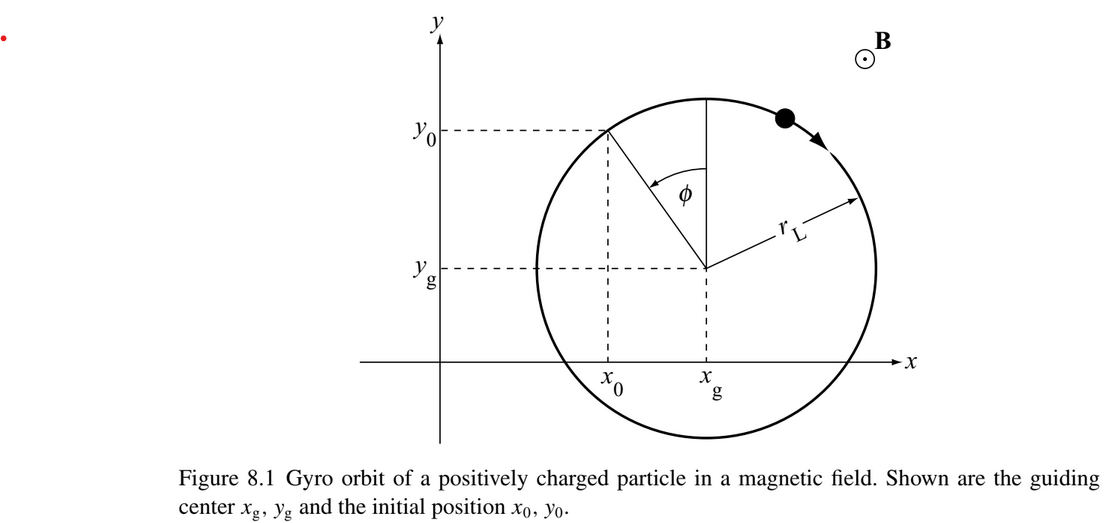
\includegraphics[width=\textwidth]{../../images/gyromotion_coordinates.png}
    \caption{Coordinates for gyro-motion (extracted from Plasma Physics and Fusion Energy, J. P. Freidberg).}
    \label{fig:gyromotion_coordiantes}
\end{figure}

\label{sec:only_B_field}
Let's orient our coordinate system such that $\Bvec$ points in the $\evec_z$ direction. Thus, the equations of motion are
\begin{subequations}
\begin{alignat}{2}
    &\frac{d v_x}{dt} = \frac{eB}{m} v_y  \qquad && v_x(0) = v_\perp \cos(\phi), \label{eq:only_B_1} \\
    &\frac{d v_y}{dt} = -\frac{eB}{m} v_x  \qquad && v_y(0) = v_\perp \sin(\phi), \label{eq:only_B_2} \\
    &\frac{d v_z}{dt} = 0  \qquad && v_z(0) = v_{||}. \label{eq:only_B_3}
\end{alignat}
\end{subequations}
The $z$ component is decoupled from the rest and has a trivial solution. For the other two components, we begin by taking the time derivative of \cref{eq:only_B_2}. Thus
\begin{equation}
    \frac{d^2 v_y}{dt^2} = -\frac{eB}{m} \frac{d v_x}{dt} = -w_c^2 v_y,
\end{equation}
where $w_c = |e|B/m$ is the gyro frequency. We know that the general solution to the above is $v_y = c_1 \cos(w_c t) + c_2 \sin(w_c t)$. If we use the ICs and assume ions, we have
\begin{equation}
\label{eq:vel_gyro_y}
    v_y = -v_\perp \sin(w_ct - \phi).
\end{equation}
Integrating \cref{eq:only_B_1} then gives
\begin{equation}
\label{eq:vel_gyro_x}
    v_x = v_\perp \cos(w_c t - \phi).
\end{equation}
The final solution, for either positive or negative charges, can be written as
\begin{align}
\label{eq:vel_gyro}
    v^{(c)}_x &= v_\perp \cos(w_c t \pm \phi) \nonumber \\
    v^{(c)}_y &= \pm v_\perp \sin(w_c t \pm \phi),
\end{align}
where upper signs correspond to a negative charge. Integrating the equations above leads to
\begin{align}
\label{eq:pos_gyro}
    x^{(c)} &= r_L \sin(w_c t \pm \phi) \nonumber \\
    y^{(c)} &= \mp r_L \cos(w_c t \pm \phi).
\end{align}
where $r_L = v_\perp/w_c$ is the gyro radius.

%--------------------------------------------
\subsection{Both $\Evec$ and $\Bvec$ fields}
%--------------------------------------------
\label{sec:E_and_B_field}
Let's orient our coordinate system such that $\Bvec$ still points along $\evec_z$. The equations of motion are
\begin{subequations}
\label{eq:single_particle_motion_EcrossB_temp1}
\begin{alignat}{2}
    &\frac{d v_x}{dt} = \frac{eE_x}{m} + \frac{eB}{m} v_y  \qquad && v_x(0) = v_\perp \cos(\phi) + \frac{E_y}{B}, \label{eq:E_and_B_1} \\
    &\frac{d v_y}{dt} = \frac{eE_y}{m} - \frac{eB}{m} v_x  \qquad && v_y(0) = v_\perp \sin(\phi) - \frac{E_x}{B}, \label{eq:E_and_B_2} \\
    &\frac{d v_z}{dt} = \frac{e E_{||}}{m}  \qquad && v_z(0) = v_{||}, \label{eq:E_and_B_3}
\end{alignat}
\end{subequations}
where we have chosen the given initial conditions simply to facilitate the math. Again, the z component is decoupled from the rest and has the trivial solution $v_z = v_{||} +  (eE_{||}/m) t$. Thus, \cref{eq:single_particle_motion_vel_general} for the $x$ and $y$ components are
\begin{align}
    \label{eq:single_particle_motion_EcrossB_temp2}
    v_x &= v_x^{(c)} + v^{(g)}_x, \nonumber \\
    v_y &= v_y^{(c)} + v^{(g)}_y.
\end{align}
We assume $v^{(g)}_x$ and $v^{(g)}_y$ are time independent. Using \cref{eq:single_particle_motion_EcrossB_temp2} in \cref{eq:single_particle_motion_EcrossB_temp1} we obtain
\begin{align}
    0 &= \frac{eE_x}{m} + \frac{eB}{m}v^{(g)}_y \nonumber \\
    0 &= \frac{eE_y}{m} - \frac{eB}{m}v^{(g)}_x.
\end{align}
Thus, $v^{(g)}_x = E_y/B$ and $v^{(g)}_y = -E_x/B$, which in vector notation can be expressed as
\begin{equation}
    \vvec^{(g)}_E = \frac{\Evec \times \Bvec}{B^2}.
\end{equation}

%------------------------------------------------------------------------
\section{Non-uniform $\Bvec$ field}
%------------------------------------------------------------------------

%--------------------------------------------
\subsection{Change in magnitude along perpendicular directions}
%--------------------------------------------
The magnetic field still points in the $\evec_z$ direction, but its magnitude changes in directions perpendicular to $\evec_z$: $B = B(q_x,q_y)$. The equations of motion are
\begin{subequations}
\begin{alignat}{2}
    &\frac{d v_x}{dt} = \frac{eB(x,y)}{m} v_y  \qquad && v_x(0) = v_\perp \cos(\phi) -\frac{v^2_\perp}{2 w_c} \left . \frac{\partial B}{\partial q_y} \right |_{x^{(g)},y^{(g)}} \frac{1}{B(x^{(g)},y^{(g)})}, \label{eq:nonuniB_1} \\
    &\frac{d v_y}{dt} = -\frac{eB(x,y)}{m} v_x  \qquad && v_y(0) = v_\perp \sin(\phi) + \frac{v^2_\perp}{2 w_c} \left . \frac{\partial B}{\partial q_x} \right |_{x^{(g)},y^{(g)}} \frac{1}{B(x^{(g)},y^{(g)})}, \label{eq:nonuniB_2} \\
    &\frac{d v_z}{dt} = 0  \qquad && v_z(0) = v_{||}. \label{eq:nonuniB_3}
\end{alignat}
\end{subequations}
In the above, the $x$ and $y$ in $B(x,y)$ are the perpendicular components of the particle's position. The $v_z$ component is decoupled from the rest and has a trivial solution. Thus, \cref{eq:single_particle_motion_vel_general,eq:single_particle_motion_pos_general} for the $x$ and $y$ components are
\begin{equation}
    \label{eq:single_particle_motion_vel_Bmag_change_perp_1}
    v_x = v_x^{(c)} + v_x^{(g)},
\end{equation}
\begin{equation}
    \label{eq:single_particle_motion_vel_Bmag_change_perp_2}
    v_y = v_y^{(c)} + v_y^{(g)},
\end{equation}
\begin{equation}
    \label{eq:single_particle_motion_pos_Bmag_change_perp_1}
    x = x^{(c)} + x^{(g)},
\end{equation}
\begin{equation}
    \label{eq:single_particle_motion_pos_Bmag_change_perp_2}
    y = y^{(c)} + y^{(g)}.
\end{equation}

We begin by employing a Taylor-series expansion for the magnetic field
\begin{equation}
    B(x,y) = B(x^{(g)}, y^{(g)}) + \left . \frac{\partial B}{\partial q_x} \right |_{x^{(g)},y^{(g)}} x^{(c)} + \left . \frac{\partial B}{\partial q_y} \right |_{x^{(g)},y^{(g)}} y^{(c)} + ...
\end{equation}
Thus, \cref{eq:nonuniB_1,eq:nonuniB_2} are now
\begin{equation}
    \frac{ d v_x}{dt} = \frac{e B(x^{(g)},y^{(g)})}{m} v_y + \frac{e}{m} \left ( \left . \frac{\partial B}{\partial q_x} \right|_{x^{(g)},y^{(g)}} x^{(c)} + \left . \frac{\partial B}{\partial q_y} \right |_{x^{(g)},y^{(g)}} y^{(c)} \right) v_y
\end{equation}
\begin{equation}
    \frac{ d v_y}{dt} = -\frac{e B(x^{(g)},y^{(g)})}{m} v_x + \frac{e}{m} \left ( \left . \frac{\partial B}{\partial q_x} \right|_{x^{(g)},y^{(g)}} x^{(c)} + \left . \frac{\partial B}{\partial q_y} \right |_{x^{(g)},y^{(g)}} y^{(c)} \right ) v_x.
\end{equation}
As before, we assume $v_x^{(g)}$, $v_y^{(g)}$ are time independent. Also, for simplicity we assume ions only. Plugging in \cref{eq:single_particle_motion_vel_Bmag_change_perp_1,eq:single_particle_motion_vel_Bmag_change_perp_2} into the above, we get
\begin{equation}
    0 = B(x^{(g)},y^{(g)}) v_y^{(g)} + \left ( \left . \frac{\partial B}{\partial q_x} \right|_{x^{(g)},y^{(g)}} x^{(c)} + \left . \frac{\partial B}{\partial q_y} \right |_{x^{(g)},y^{(g)}} y^{(c)} \right) \left ( v_y^{(c)} + v_y^{(g)} \right),
\end{equation}
\begin{equation}
    0 = -B(x^{(g)},y^{(g)}) v_x^{(g)} + \left ( \left . \frac{\partial B}{\partial q_x} \right|_{x^{(g)},y^{(g)}} x^{(c)} + \left . \frac{\partial B}{\partial q_y} \right |_{x^{(g)},y^{(g)}} y^{(c)} \right ) \left ( v_x^{(c)} + v_x^{(g)} \right ).
\end{equation}
We assume $v_x^{(g)} \ll v_x^{(c)}$ and $v_y^{(g)} \ll v_y^{(c)}$. Thus, the above becomes
\begin{equation}
    \label{eq:single_particle_motion_Bmag_change_perp_temp1}
    0 = B(x^{(g)},y^{(g)}) v_y^{(g)} + \left ( \left . \frac{\partial B}{\partial q_x} \right|_{x^{(g)},y^{(g)}} x^{(c)} + \left . \frac{\partial B}{\partial q_y} \right |_{x^{(g)},y^{(g)}} y^{(c)} \right) v_y^{(c)},
\end{equation}
\begin{equation}
    \label{eq:single_particle_motion_Bmag_change_perp_temp2}
    0 = -B(x^{(g)},y^{(g)}) v_x^{(g)} + \left ( \left . \frac{\partial B}{\partial q_x} \right|_{x^{(g)},y^{(g)}} x^{(c)} + \left . \frac{\partial B}{\partial q_y} \right |_{x^{(g)},y^{(g)}} y^{(c)} \right ) v_x^{(c)}.
\end{equation}
We now use the definitions in \cref{eq:vel_gyro} and \cref{eq:pos_gyro}. For example, with those definitions we can show that 
\begin{align}
     x^{(c)} v_y^{(c)} &= \left[ r_L \sin (w_c t - \phi) \right] \left[ -v_\perp \sin (w_ct - \phi) \right] \nonumber \\
    & = -\frac{ v^2_\perp}{w_c} \sin^2(w_c t - \phi) \nonumber \\
    & = -\frac{ v^2_\perp}{2 w_c} \{1 - \cos [ 2 (w_c t - \phi)] \}
\end{align}
Similar derivations can be carried out for $y^{(c)} v_y^{(c)}$, $x^{(c)} v_x^{(c)}$, and $y^{(c)} v_x^{(c)}$. Thus, \cref{eq:single_particle_motion_Bmag_change_perp_temp1,eq:single_particle_motion_Bmag_change_perp_temp2} become 
\begin{multline}
    0 = B(x^{(g)},y^{(g)}) v_y^{(g)} -\frac{ v^2_\perp}{2 w_c} \left . \frac{\partial B}{\partial q_x} \right |_{x^{(g)},y^{(g)}} \{1 - \cos [ 2 (w_c t - \phi)] \} \\
    - \frac{ v^2_\perp}{2 w_c} \left .\frac{\partial B}{\partial q_y} \right |_{x^{(g)},y^{(g)}} \sin [ 2(w_ct - \phi)],
\end{multline}
\begin{multline}
    0 = -B(x^{(g)},y^{(g)}) v_x^{(g)} -\frac{ v^2_\perp}{2 w_c} \left . \frac{\partial B}{\partial q_x} \right |_{x^{(g)},y^{(g)}} \sin [ 2 (w_c t - \phi)] \\
    - \frac{ v^2_\perp}{2 w_c} \left .\frac{\partial B}{\partial q_y} \right |_{x^{(g)},y^{(g)}} \{ 1 + \cos [ 2(w_ct - \phi)] \}.
\end{multline}
We neglect the oscillatory terms containing the sines and cosines---if it was not possible to neglect them, then the assumption that $v^{(g)}_x$, $v^{(g)}_y$ are time independent would not hold. Thus,
\begin{subequations}
\begin{alignat}{2}
    0 &= B(x^{(g)},y^{(g)}) v_y^{(g)} - \frac{ v^2_\perp}{2 w_c} \left . \frac{\partial B}{\partial q_x} \right |_{x^{(g)},y^{(g)}} \nonumber \\
    0 &= -B(x^{(g)},y^{(g)}) v_x^{(g)} -\frac{ v^2_\perp}{2 w_c} \left . \frac{\partial B}{\partial q_y} \right |_{x^{(g)},y^{(g)}} . 
\end{alignat}
\end{subequations}
Solving for the guiding center velocities, we finally have
\begin{align}
    v_x^{(g)} &= -\frac{v^2_\perp}{2 w_c} \left . \frac{\partial B}{\partial q_y} \right |_{x^{(g)},y^{(g)}} \frac{1}{B(x^{(g)},y^{(g)})} \nonumber \\
    v_y^{(g)} &= \frac{v^2_\perp}{2 w_c} \left . \frac{\partial B}{\partial q_x} \right |_{x^{(g)},y^{(g)}} \frac{1}{B(x^{(g)},y^{(g)})} . 
\end{align}
In vector notation, this is written as
\begin{equation}
    \vvec^{(g)}_{\nabla B} = \mp \frac{v^2_\perp}{2 w_c} \frac{ \Bvec \times \nabla B }{B^2}.
\end{equation}
In the above, the fields and $w_c$ are evaluated at $(x^{(g)},y^{(g)})$.

%--------------------------------------------
\subsection{Change in magnitude along parallel directions}
%--------------------------------------------
Ideally, one would introduce a gradient only in the direction parallel to the magnetic field, that is, one would have $\Bvec = B(q_z) \evec_z$. However, due to Gauss's law, this is too restrictive and instead we generalize and use $\Bvec = B_x \evec_x + B_z \evec_z$, where $B_x = B_x(q_x,q_z)$ and $B_z = B_z(q_x,q_z)$. Thus, the equations of motion are
\begin{align}
    \frac{dv_x}{dt} &= \frac{e}{m} v_y B_z(x,z) , \label{eq:par_grad_vx_inter}\\
    \frac{dv_y}{dt} &= -\frac{e}{m} [v_x B_z(x,z) - v_z B_x(x,z)] , \label{eq:par_grad_vy_inter}\\
    \frac{dv_z}{dt} &= -\frac{e}{m} v_y B_x(x,z) \label{eq:par_grad_vz_inter}.
\end{align}
However, the $z$ direction no longer corresponds to the parallel direction, since the magnetic field also has a component along the $x$ direction. To account for this, we will introduce a rotating reference frame, in which one of the axis will always be aligned with the magnetic field vector, and thus would denote the parallel direction. In the original static reference frame the unit vectors are $(\evec_x, \evec_y, \evec_z)$ and the velocity components are $(v_x, v_y, v_x)$, whereas in this new rotating reference frame the unit vectors are $(\evec_{\perp1}, \evec_{\perp2}, \bvec)$ and the velocity components are $(v_{\perp1}, v_{\perp2}, v_{||})$. 

The rotating reference frame is described by the rotation matrix
\begin{equation}
    \Qvec(t) = \begin{bmatrix} b_x & 0 & b_z \\ 0 & 1 & 0 \\ b_z & 0 & -b_x \end{bmatrix},
\end{equation}
where $b_x = b_x(t)$ and $b_y = b_y(t)$ are given by
\begin{equation}
    b_x = \frac{B_x(x,z)}{B(x,z)} \qquad b_z = \frac{B_z(x,z)}{B(x,z)} \label{eq:bvec_components}
\end{equation}
In the above, $B(x,z) = [ B_x^2(x,z) + B_z^2(x,z) ]^{1/2}$. As an example, the matrix above leads to the following transformations for the unit vectors and velocities in the rotating reference frame 
\begin{align}
    \bvec &= b_x \evec_x + b_z \evec_z \\
    \evec_{\perp2} &= \evec_y \\
    \evec_{\perp1} &= b_z \evec_x - b_x \evec_z = \evec_{\perp2} \times \bvec,
\end{align}
\begin{align}
    v_{||} &= b_x v_x + b_z v_z \label{eq:par_grad_vel_trans_1}\\
    v_{\perp2} &= v_y \label{eq:par_grad_vel_trans_2}\\
    v_{\perp1} &= b_z v_x - b_x v_z. \label{eq:par_grad_vel_trans_3}
\end{align}
Using the transformation rule for the acceleration of a particle, but for some reason neglecting the coriollis and centrifugal forces, we obtain for the velocity derivatives
\begin{align}
    \frac{dv_{||}}{dt} &= \frac{dv_x}{dt} b_x + \frac{dv_z}{dt} b_z  - K v_{\perp1} \\
    \frac{dv_{\perp2}}{dt} &= \frac{dv_y}{dt}\\
    \frac{dv_{\perp1}}{dt} &= \frac{dv_x}{dt} b_z - \frac{dv_z}{dt} b_x + K v_{||},
\end{align}
where $K = K(t)$ is given by $K = b_x db_z/dt - b_z db_x/dt$. Using \cref{eq:par_grad_vx_inter,eq:par_grad_vy_inter,eq:par_grad_vz_inter} in the above leads to
\begin{align}
    \frac{d v_{||}}{dt} &= \frac{e}{m} v_y [B_z(x,z) b_x - B_x(x,z) b_z] - Kv_{\perp1} \\
    \frac{dv_{\perp2}}{dt} &= -\frac{eB}{m} (v_x b_z - v_z b_x) \\
    \frac{dv_{\perp1}}{dt} &= \frac{e}{m} v_y [B_z(x,z) b_z + B_x(x,z) b_x] + Kv_{||} 
\end{align}
Using the definitions for $b_x$ and $b_z$ in \cref{eq:bvec_components}, as well as the expressions for $v_{\perp1}$, $v_{\perp2}$ in \cref{eq:par_grad_vel_trans_2,eq:par_grad_vel_trans_3}, we get
\begin{align}
    \frac{d v_{||}}{dt} &= -Kv_{\perp1}, \label{eq:par_grad_vpar_inter} \\
    \frac{dv_{\perp2}}{dt} &= -w_c v_{\perp1}, \label{eq:par_grad_v2_inter} \\
    \frac{dv_{\perp1}}{dt} &= w_c v_{\perp2} + K v_{||}, \label{eq:par_grad_v1_inter}
\end{align}
where $w_c = w_c(t)$ is given by $w_c = e B(x,z) / m$.

We now introduce a time transformation to simplify the equations above. To do so, we introduce the following variables
\begin{gather}
    \hat{v}_{||} = \hat{v}_{||}(\tau) \qquad \hat{v}_{\perp2} = \hat{v}_{\perp2}(\tau) \qquad \hat{v}_{\perp1} = \hat{v}_{\perp1}(\tau) \\
    \hat{x} = \hat{x}(\tau) \qquad \hat{z} = \hat{z}(\tau)
\end{gather}
such that
\begin{gather}
    v_{||} = \hat{v}_{||}(h(t)) \qquad v_{\perp2} = \hat{v}_{\perp2}(h(t)) \qquad v_{\perp1} = \hat{v}_{\perp1}(h(t)) \\
    x = \hat{x}(h(t)) \qquad z = \hat{z}(h(t)).
\end{gather}
The function $h(t)$ is given by
\begin{equation}
    h(t) = \int_0^t w_c(t') dt'.
\end{equation}
We also show that
\begin{equation}
    b_x = \frac{B_x(x,z)}{B(x,z)} = \frac{B_x(\hat{x}(h(t)),\hat{z}(h(t)))}{B(\hat{x}(h(t)),\hat{z}(h(t)))},
\end{equation}
and thus
\begin{equation}
    \frac{db_x}{dt} = \frac{dh(t)}{dt} \frac{d}{d\tau} \left [ \frac{B_x(\hat{x},\hat{z})}{B(\hat{x},\hat{z})} \right ]_{\tau = h(t)} = w_c \left .\frac{d \hat{b}_x}{d\tau} \right|_{\tau = h(t)},
\end{equation}
where $\hat{b}_x =\hat{b}_x(\tau)$ is given by $\hat{b}_x= B_x(\hat{x},\hat{z}) / B(\hat{x},\hat{z})$. The analogous holds for $b_z$. This allows us to write
\begin{equation}
    K = w_c \left ( \hat{b}_x \frac{d\hat{b}_z}{d \tau} - \hat{b}_z \frac{d\hat{b}_x}{d \tau} \right )_{\tau = h(t)} = w_c \left. \hat{K} \right |_{\tau = h(t)},
\end{equation}
where $\hat{K} = \hat{K}(\tau)$ is given by $\hat{K} = \hat{b}_x d\hat{b}_z/d\tau - \hat{b}_z d\hat{b}_x/d\tau$. With these transformation, \cref{eq:par_grad_vpar_inter,eq:par_grad_v2_inter,eq:par_grad_v1_inter} are re-written as
\begin{align}
    \frac{d\hat{v}_{||}}{d\tau} &= -\hat{K} \hat{v}_{\perp1},\\
    \frac{d\hat{v}_{\perp2}}{d\tau} &= -\hat{v}_{\perp1},\\
    \frac{d\hat{v}_{\perp1}}{d\tau} &= \hat{v}_{\perp2} + \hat{K} \hat{v}_{||}.
\end{align}

We now simplify $B_z$ so that $B_z = B_z(q_z)$. To be consistent with Gauss's law, we require $B_x = B_x(q_x,q_y)$ where $B_x = -q_x dB_z/dq_z$. With these simplified forms, we have
\begin{align}
    \hat{K} &= -\hat{b}_z^2 \frac{d}{d\tau} \left ( \frac{\hat{b}_x}{\hat{b}_z} \right ) \\
    &= -\frac{B_z^2(\hat{z})}{B^2(\hat{x},\hat{z})} \frac{d}{d\tau} \left ( \frac{B_x(\hat{x},\hat{z})}{B_z(\hat{z})} \right ) \\
    &= \frac{B_z^2(\hat{z})}{B^2(\hat{x},\hat{z})} \frac{d}{d\tau} \left [ \hat{x}  \left ( \frac{1}{B_z} \frac{dB_z}{dq_z} \right )_{q_z = \hat{z}} \right ].
\end{align}
We now use the long-thin approximation. For this approximation, we assume that $B_x / B_z \ll 1$, and also that $\frac{1}{B_z} \frac{dB_z}{dq_z}$ changes very slowly. We thus have
\begin{equation}
\label{eq:par_grad_k_inter}
    \hat{K} \approx \frac{d \hat{x}}{d\tau} \left ( \frac{1}{B_z} \frac{dB_z}{dq_z} \right)_{q_z = \hat{z}}.
\end{equation}
Also, using the long-thin approximation in \cref{eq:par_grad_vel_trans_1,eq:par_grad_vel_trans_3} allows us to write
\begin{align}
    v_{||} &\approx v_z = \frac{dz}{dt} = \left ( \frac{d\hat{z}}{d\tau} \right )_{\tau = h(t)} w_c \\
    v_{\perp1} & \approx v_x = \frac{dx}{dt} = \left ( \frac{d \hat{x}}{d\tau} \right )_{\tau = h(t)} w_c.
\end{align}
Evaluating the above at $t = h^{-1}(\tau)$, and defining $\hat{w}_c(\tau)$ from $w_c = \hat{w}_c(h(t))$, we obtain
\begin{align}
    \hat{v}_{||} &\approx  \frac{d\hat{z}}{d\tau}  \hat{w}_c \\
    \hat{v}_{\perp1} & \approx \frac{d \hat{x}}{d\tau} \hat{w}_c.
\end{align}
We also note that
\begin{equation}
    \frac{d B_z(\hat{z})}{d\tau} = \left ( \frac{dB_z}{dq_z} \right )_{q_z = \hat{z}} \frac{d \hat{z}}{d\tau}.
\end{equation}
Using the expressions above in \cref{eq:par_grad_k_inter}, one can approximate $\hat{K}$ using either of the two forms below
\begin{equation}
    \hat{K} \approx \frac{\hat{v}_{\perp1}}{\hat{w}_c B_z(\hat{z})} \left ( \frac{dB_z}{dq_z} \right )_{q_z = \hat{z}} \approx \frac{\hat{v}_{\perp1}}{\hat{v}_{||} B_z(\hat{z})} \frac{dB_z(\hat{z})}{d\tau} .
\end{equation}
We thus write the governing equations for the velocities as
\begin{align}
    \frac{d\hat{v}_{||}}{d\tau} &= -\frac{\hat{v}^2_{\perp1}}{\hat{w}_c B_z(\hat{z})} \left ( \frac{dB_z}{dq_z} \right )_{q_z = \hat{z}} ,\label{eq:par_grad_vpar_thin}\\
    \frac{d\hat{v}_{\perp2}}{d\tau} &= -\hat{v}_{\perp1}, \label{eq:par_grad_v2_thin} \\
    \frac{d\hat{v}_{\perp1}}{d\tau} &= \hat{v}_{\perp2} + \frac{\hat{v}_{\perp1}}{B_z(\hat{z})} \frac{dB_z(\hat{z})}{d\tau}. \label{eq:par_grad_v1_thin}
\end{align}

We now assume the solution for the perpendicular velocities is of the form
\begin{align}
    \hat{v}_{\perp1} &= \hat{v}_\perp \cos [\tau + \hat{\epsilon}] \\
    \hat{v}_{\perp2} &= -\hat{v}_\perp \sin [\tau + \hat{\epsilon}],
\end{align}
where $\hat{v}_\perp = \hat{v}_\perp(\tau)$ and $\hat{\epsilon} = \hat{\epsilon}(\tau)$. Plugging these two assumed solutions into \cref{eq:par_grad_v2_thin,eq:par_grad_v1_thin}, and using some simple algebra, gives
\begin{equation}
    \frac{d\hat{v}_\perp}{d\tau} = \frac{\hat{v}_\perp}{2 B_z(\hat{z})} \frac{dB_z(\hat{z})}{d\tau} \left \{ 1 + \cos [2 (\tau + \hat{\epsilon})] \right \}.
\end{equation}
The above can be re-arranged and expressed as
\begin{equation}
\label{eq:par_grad_mu_evol}
    \frac{d \ln \hat{\mu}}{d\tau} = \frac{d \ln B_z(\hat{z}) }{d\tau} \cos [2 (\tau + \hat{\epsilon})],
\end{equation}
where $\hat{\mu} = \hat{\mu}(\tau)$ is the adiabatic invariant, and is given by
\begin{equation}
    \hat{\mu} = \frac{m \hat{v}^2_\perp}{2 B_z(\hat{z})}.
\end{equation}
Integrating \cref{eq:par_grad_mu_evol} from $\tau_1$ to $\tau_2$ gives
\begin{equation}
    \ln \hat{\mu}(\tau_2) - \ln \hat{\mu}(\tau_1) = \left . \ln [B_z(\hat{z})] \cos [2(\tau + \hat{\epsilon})] \right |^{\tau_2}_{\tau_1} + \int_{\tau_1}^{\tau_2} 2 \ln [ B_z(\hat{z}) ] \sin [2(\tau + \hat{\epsilon})] d\tau.
\end{equation}
Picking $\tau_1$ and $\tau_2$ such that $[\tau_2 + \hat{\epsilon}(\tau_2)] - [\tau_1 + \hat{\epsilon}(\tau_1)] = 2 \pi$, and assuming $B(\hat{z})$ doesn't change significantly from $\tau_1$ to $\tau_2$, gives $\hat{\mu}(\tau_2) = \hat{\mu}(\tau_1)$, that is, $\hat{\mu}$ is constant over one gyro-period. One can also define
\begin{equation}
    \mu = \frac{m v_\perp^2}{2B_z(z)}
\end{equation}
where $\mu = \mu(t)$ and $v_\perp = v_\perp(t)$. Given that $v_\perp = \hat{v}_\perp(h(t))$, we have $\mu = \hat{\mu}(h(t))$. Thus, $\hat{\mu}(\tau_2) = \hat{\mu}(\tau_1)$ translates to $\mu(t_2) = \mu(t_1)$, where $t_2 = h^{-1}(\tau_2)$ and $t_1 = h^{-1}(\tau_1)$.

Finally, we focus not on the perpendicular velocities but the parallel velocity. Plugging-in the assumed solutions in the governing \cref{eq:par_grad_vpar_thin} gives
\begin{equation}
    \frac{d\hat{v}_{||}}{d\tau} = -\frac{\hat{v}^2_{\perp}}{2\hat{w}_c B_z(\hat{z})} \left ( \frac{dB_z}{dq_z} \right )_{q_z = \hat{z}} \{ 1 + \cos [2(\tau + \hat{\epsilon})] \}.
\end{equation}
We now average the above from $\tau_1$ to $\tau_2$ while assuming $B(\hat{z})$, $d\hat{v}_{||}/d\tau$ and $\hat{v}^2_\perp$ do not change significantly during that time scale. Note that since this is an average, we are not just integrating from $\tau_1$ to $\tau_2$, but we are also dividing by $\tau_2 - \tau_1$. After  averaging, we obtain
\begin{equation}
    \frac{d\hat{v}_{||}}{d\tau} = -\frac{\hat{v}^2_{\perp}}{2\hat{w}_c B_z(\hat{z})} \left ( \frac{dB_z}{dq_z} \right )_{q_z = \hat{z}} .
\end{equation}
or
\begin{equation}
    m \frac{d\hat{v}_{||}}{d\tau} = -\frac{\hat{\mu}}{\hat{w}_c} \left ( \frac{dB_z}{dq_z} \right )_{q_z = \hat{z}} .
\end{equation}
Converting back to time $t$ gives
\begin{equation}
    m \frac{dv_{||}}{dt} = -\mu \left ( \frac{dB_z}{dq_z} \right )_{q_z = z} .
\end{equation}


%--------------------------------------------
\subsection{Change in direction}
%--------------------------------------------
Rather than writing \cref{eq:single_particle_motion} in terns if its components as done in previous sections, we leave the equation in vector form. Expressing the velocity as $\vvec = \vvec_\perp + v_{||} \bvec$ and assuming no electric field, we write \cref{eq:single_particle_motion} as
\begin{equation}
    \frac{d}{dt} ( \vvec_\perp + v_{||} \bvec) = \mp w_c (\vvec_\perp + v_{||} \bvec ) \times \bvec,
\end{equation}
where upper sign corresponds to negative charge and lower sign to positive charge. For simplicity we will assume positively charged particles only. We then cross both sides of the above by $\bvec$, that is
\begin{equation}
    \bvec \times \left \{ \left [ \frac{d}{dt} ( \vvec_\perp + v_{||} \bvec) - w_c ( \vvec_\perp + v_{||} \bvec) \times \bvec \right ] \times \bvec \right \} = 0.
\end{equation}
The above is simplified using the following three manipulations
\begin{align}
    \bvec \times \left \{ \left [ w_c ( \vvec_\perp + v_{||} \bvec) \times \bvec \right ] \times \bvec \right \} &= \bvec \times \left \{ \left [ w_c \vvec_\perp \times \bvec \right ] \times \bvec \right \} \nonumber \\
    & = -\bvec \times \left \{ w_c \vvec_\perp ( \bvec \cdot \bvec) - \bvec (\bvec \cdot w_c \vvec_\perp ) \right \} \nonumber \\
    & = w_c \vvec_\perp \times \bvec.
\end{align}
\begin{equation}
    \bvec \times \left \{ \left [ \frac{d\vvec_\perp}{dt} \right ] \times \bvec \right \} = \frac{d \vvec_\perp}{dt}( \bvec \cdot \bvec) - \bvec \left ( \bvec \cdot \frac{d\vvec_\perp}{dt} \right ) = \left ( \frac{d \vvec_\perp}{dt} \right )_\perp.
\end{equation}
\begin{align}
    \bvec \times \left \{ \left [ \frac{d v_{||} \bvec}{dt} \times \bvec \right ] \right \} &= v_{||} \bvec \times \left \{ \left [ \frac{ d\bvec}{dt} \times \bvec \right ] \right \} \nonumber \\
    & = v_{||} \left [ \frac{d \bvec}{dt} ( \bvec \cdot \bvec) - \bvec \left ( \bvec \cdot \frac{d \bvec}{dt} \right ) \right ] \nonumber \\
    & = v_{||} \left [ \frac{d \bvec}{dt} - \bvec \left ( \frac{1}{2} \frac{d \bvec \cdot \bvec}{dt} \right ) \right ] \nonumber \\
    & = v_{||} \frac{d \bvec}{dt}
\end{align}
Thus, we have
\begin{equation}
\label{eq:curvature_1}
    \left ( \frac{ d \vvec_\perp}{dt} \right )_\perp - w_c \vvec_\perp \times \bvec = -v_{||} \frac{d\bvec}{dt}.
\end{equation}
As shown in Freidberg
\begin{equation}
    \frac{d \bvec(\xvec(t))}{dt} = \frac{d \xvec(t)}{dt} \cdot \nabla \bvec = \vvec \cdot \nabla \bvec = \vvec_\perp \cdot \nabla \bvec + v_{||} \bvec \cdot \nabla \bvec,
\end{equation}
where $\nabla \bvec$ is evaluated at $\xvec = \xvec(t)$. Thus, \cref{eq:curvature_1} becomes
\begin{equation}
\label{eq:curvature_2}
    \left ( \frac{ d \vvec_\perp}{dt} \right )_\perp - w_c \vvec_\perp \times \bvec = -v_{||} \vvec_\perp \cdot \nabla \bvec - v_{||}^2 \bvec \cdot \nabla \bvec.
\end{equation}
As was done for the other drifts, we assume the solution is of the form $\vvec_\perp = \vvec^{(c)} + \vvec^{(g)}$, where we assume again that $\vvec^{(g)}$ is time independent. The term $\vvec^{(c)}$ corresponds to gyro-motion in a rotating reference frame, and is thus given by 
\begin{equation}
    \vvec^{(c)} = v^{(c)}_{\perp1} \evec_{\perp1} + v^{(c)}_{\perp2} \evec_{\perp2},
\end{equation}
where $\evec_{\perp1}$ and $\evec_{\perp2}$ are orthogonal to $\bvec$ and thus rotate in time. $v^{(c)}_{\perp1}$ is given by \cref{eq:vel_gyro_x} and $v^{(c)}_{\perp2}$ by \cref{eq:vel_gyro_y}. We note that, in the non-rotating reference frame, $\vvec^{(c)}$ is expressed as $\vvec^{(c)} = v^{(c)}_x \evec_x + v^{(c)}_y \evec_y + v^{(c)}_z \evec_z$. We now prove that $\vvec_\perp^{(c)}$ is the solution to the two terms on the left-hand side of \cref{eq:curvature_2}. To show this we first use the transformation rule for the acceleration of a particle in a rotating reference frame, but for some reason ignore the coriollis and centrifugal terms. Thus
\begin{align}
    \frac{d \vvec^{(c)}}{dt} &= \frac{dv^{(c)}_x}{dt} \evec_x + \frac{dv^{(c)}_y}{dt} \evec_y + \frac{dv^{(c)}_z}{dt} \evec_z \nonumber \\ &= \frac{dv^{(c)}_{\perp1}}{dt} \evec_{\perp1} + \frac{dv^{(c)}_{\perp2}}{dt} \evec_{\perp2} + 2\Omega \times \vvec^{(c)}.
\end{align}
We do not allow the rotating reference frame to rotate about the $\bvec$ axis. Thus, $\Omega = \Omega_{\perp1} \evec_{\perp1} + \Omega_{\perp2} \evec_{\perp2}$. Given that $\Omega$ and $\vvec^{(c)}$ are in the same plane, $\Omega \times \vvec^{(c)}$ must point in the $\bvec$ direction. Thus, 
\begin{equation}
    \left ( \frac{d \vvec^{(c)}}{dt} \right )_\perp = \frac{dv^{(c)}_{\perp1}}{dt} \evec_{\perp1} + \frac{dv^{(c)}_{\perp2}}{dt} \evec_{\perp2}.
\end{equation}
This allows us to show that 
\begin{equation}
    \left ( \frac{d \vvec^{(c)}}{dt} \right )_\perp - w_c \vvec^{(c)} \times \bvec = \frac{dv^{(c)}_{\perp1}}{dt} \evec_{\perp1} + \frac{dv^{(c)}_{\perp2}}{dt} \evec_{\perp2} - w_c v^{(c)}_{\perp2} \evec_{\perp1} + w_c v^{(c)}_{\perp1} \evec_{\perp2} = 0.
\end{equation}
We now plug in $\vvec_\perp = \vvec^{(c)} + \vvec^{(g)}$ in \cref{eq:curvature_2} to obtain
\begin{equation}
\label{eq:curvature_3}
    -w_c \vvec^{(g)} \times \bvec = - v_{||} \vvec_\perp \cdot \nabla \bvec - v_{||}^2 \bvec \cdot \nabla \bvec.
\end{equation}
As explained in Freidberg, the term $v_{||} \vvec_\perp \cdot \nabla \bvec$ leads to small modifications of the gyro motion, but does not lead to a drift of the particles, and thus is ignored. Taking the cross product of \cref{eq:curvature_3} with $\bvec$ finally gives the curvature drift
\begin{equation}
    \vvec^{(g)}_\kappa = \pm \frac{v_{||}^2}{w_c} \frac{( \bvec \cdot \nabla \bvec ) \times \Bvec}{B}.
\end{equation}

We now show that, if we assume $\nabla \times \Bvec = 0$, the grad-B drift 
\begin{equation}
    \vvec^{(g)}_{\nabla B} = \mp \frac{v^2_\perp}{2 w_c} \frac{\Bvec \times \nabla B}{B^2}
\end{equation}
can be written in the same form as the curvature drift. We begin by showing that
\begin{equation}
    \Bvec \times \nabla B = \Bvec \times \nabla \left ( \Bvec \cdot \Bvec \right )^{1/2} = \Bvec \times \frac{1}{2B} \nabla \left ( \Bvec \cdot \Bvec \right ).
\end{equation}
We now use the vector identity $\nabla (\Bvec \cdot \Bvec ) = 2 \Bvec \times (\nabla \times \Bvec) + 2 \Bvec \cdot \nabla \Bvec$, and assume magnetic curl of zero to obtain
\begin{align}
    \Bvec \times \nabla B &= \Bvec \times \frac{1}{B} \Bvec \cdot \nabla \Bvec \nonumber \\
    &= \Bvec \times \bvec \cdot \nabla (B \bvec) \nonumber \\
    &= \Bvec \times \left (\bvec \cdot \nabla B \right ) \bvec + \Bvec \times B \left (\bvec \cdot \nabla \bvec \right ) \nonumber \\
    &= -B \left ( \bvec \cdot \nabla \bvec \right ) \times \Bvec.
\end{align}
Thus, the grab-B drift can be written as 
\begin{equation}
    \vvec^{(g)}_{\nabla B} = \pm \frac{v^2_\perp}{2 w_c} \frac{(\bvec \cdot \nabla \bvec) \times \Bvec}{B}.
\end{equation}

%------------------------------------------------------------------------
\section{Non-uniform $\Evec$ field}
%------------------------------------------------------------------------

%------------------------------------------------------------------------
\section{Time-varying $\Evec$ field}
%------------------------------------------------------------------------
Consider the scenario used in \cref{sec:E_and_B_field}, but with a time varying electric field. The equations of motion are
\begin{subequations}
\label{eq:time_var_E_temp1}
\begin{alignat}{2}
    &\frac{d v_x}{dt} = \frac{eE_x(t)}{m} + \frac{eB}{m} v_y  \qquad && v_x(0) = v_\perp \cos(\phi) + \frac{E_y(t)}{B} + \frac{m}{eB^2}\frac{dE_x(t)}{dt},  \\
    &\frac{d v_y}{dt} = \frac{eE_y(t)}{m} - \frac{eB}{m} v_x  \qquad && v_y(0) = v_\perp \sin(\phi) - \frac{E_x(t)}{B} + \frac{m}{eB^2}\frac{dE_y(t)}{dt},  \\
    &\frac{d v_z}{dt} = \frac{e E_{||}(t)}{m}  \qquad && v_z(0) = v_{||}, 
\end{alignat}
\end{subequations}
where again we chose the initial conditions simply to be consistent with the solution that we'll derive. The parallel velocity is independent of the perpendicular velocities, and we won't worry about it for now. To solve for the perpendicular velocities, we again assume the general solution is 
\begin{align}
\label{eq:time_var_temp2}
    v_x = v_x^{(c)} + v_x^{(g)} \nonumber \\
    v_y = v_y^{(c)} + v_y^{(g)} 
\end{align}
but now do not assume $v_x^{(g)}$ and $v_y^{(g)}$ are time independent. We expand $v_i^{(g)}$ as 
\begin{equation}
    v_i^{(g)} = v^{(g,1)}_i +  v^{(g,2)}_i + ...,
\end{equation}
where $v_i^{(g,\alpha)} \sim \epsilon v_i^{(g,\alpha-1)}$, and the small parameter $\epsilon$ follows from assuming 
\begin{equation}
\label{eq:time_var_E_temp3}
    \frac{1}{v^{(g,\alpha)}_i} \frac{d v^{(g,\alpha)}_i}{dt} \sim \epsilon w_c.
\end{equation}
That is, the time scale associated with the rate of change of all of the $v^{(g,\alpha)}_i$ components is much larger than the time scale of the gyro-motion. In other words, we assume particles gyrate faster than how quickly their drift velocity changes. Using \cref{eq:time_var_temp2} in \cref{eq:time_var_E_temp1} leads to
\begin{align}
    \frac{dv_x^{(g,1)}}{dt} + \frac{dv_x^{(g,2)}}{dt} &= \frac{e E_x(t)}{m} + \frac{eB}{m} v_y^{(g,1)} + \frac{eB}{m} v_y^{(g,2)} \nonumber \\
    \frac{dv_y^{(g,1)}}{dt} + \frac{dv_y^{(g,2)}}{dt} &= \frac{e E_y(t)}{m} - \frac{eB}{m} v_x^{(g,1)} - \frac{eB}{m} v_x^{(g,2)}.
\end{align}
Collecting lowest order terms
\begin{align}
    0 &= \frac{eE_x(t)}{m} + \frac{eB}{m} v_y^{(g,1)}  \nonumber \\
    0 &= \frac{eE_y(t)}{m} - \frac{eB}{m} v_x^{(g,1)} ,
\end{align}
and thus $v^{(g,1)}_x = E_y(t) / B$ and $v^{(g,1)}_y = -E_x(t) / B$, which in vector notation is
\begin{equation}
    \vvec^{(g,1)} = \frac{\Evec(t) \times \Bvec}{B^2}.
\end{equation}
Collecting first order terms 
\begin{align}
    \frac{dv_x^{(g,1)}}{dt} &= \frac{eB}{m} v_y^{(g,2)} \nonumber \\
    \frac{dv_y^{(g,1)}}{dt} &= -\frac{eB}{m} v_x^{(g,2)},
\end{align}
and thus $v_x^{(g,2)} = (m/eB^2)dE_x(t)/dt$ and $v_y^{(g,2)} = (m/eB^2) dE_y(t)/dt$, which in vector notation is
\begin{equation}
    \label{eq:particle_polarization_drift}
    \vvec^{(g,2)} = \mp \frac{1}{w_c B}\frac{d\Evec_\perp}{dt}.
\end{equation}
We note that, by looking at the solutions for $v_x^{(g,1)}$ and $v_y^{(g,1)}$, the assumption in \cref{eq:time_var_E_temp3} is equivalent to stating that the electric field changes slowly. 

%------------------------------------------------------------------------
\section{Time-varying $\Bvec$ field}
%------------------------------------------------------------------------
Let's assume the magnetic field points in the $z$ direction again. Using Faraday's law, we have
\begin{equation}
    \left(\frac{\partial E_z}{\partial q_y} - \frac{\partial E_y}{\partial q_z} \right) \evec_x - \left(\frac{\partial E_z}{\partial q_x} - \frac{\partial E_x}{\partial q_z} \right) \evec_y + \left(\frac{\partial E_y}{\partial q_x} - \frac{\partial E_x}{\partial q_y} \right) \evec_z = -\frac{\partial B}{\partial t} \evec_z.
\end{equation}
To satisfy the above, we set $E_z = 0$, and $E_x = E_x(q_x,q_y,t)$, $E_y = E_y(q_x,q_y,t)$. That is, a time varying magnetic field requires a time and spatially varying electric field. 

We will further simplify our analysis by having $E_x = 0$ and $E_y = E_y(q_x,t)$. Thus, the equations of motion are
\begin{align}
    \frac{dv_x}{dt} &= \frac{eB(t)}{m} v_y, \\
    \frac{dv_y}{dt} &= \frac{eE_y(x,t)}{m} - \frac{eB(t)}{m}v_x,
\end{align}
with $v_z$ constant. As done in previous sections, the velocities and positions are decomposed as follows
\begin{equation}
    v_x = v_x^{(c)} + v_x^{(g)},
\end{equation}
\begin{equation}
    v_y = v_y^{(c)} + v_y^{(g)},
\end{equation}
\begin{equation}
    x = x^{(c)} + x^{(g)},
\end{equation}
\begin{equation}
    y = y^{(c)} + y^{(g)}.
\end{equation}
The electric field is then linearized using a Taylor-series expansion about the guiding center,
\begin{align}
    \frac{dv_x}{dt} &= \frac{eB(t)}{m} v_y \\
    \frac{dv_y}{dt} &= \frac{e}{m} \left [ E_y \left ( x^{(g)},t \right ) + \left .\frac{\partial E_y}{\partial q_x} \right |_{x^{(g)}} x^{(c)} \right ] - \frac{eB(t)}{m}v_x,
\end{align}
We assume positive ions for simplicity and re-write the above as
\begin{align}
    \frac{dv_x}{dt} &= w_c v_y \\
    \frac{dv_y}{dt} &= \frac{w_c}{B(t)} \left [ E_y \left ( x^{(g)},t \right ) + \left .\frac{\partial E_y}{\partial q_x} \right |_{x^{(g)}} x^{(c)} \right ] - w_c v_x.
\end{align}
where $w_c = w_c(t)$. We introduce new variables 
\begin{gather}
    \hat{v}_x = \hat{v}_x(\tau) \qquad \hat{v}_y = \hat{v}_y(\tau) \qquad \hat{x}^{(c)} = \hat{x}^{(c)}(\tau) \qquad \hat{x}^{(g)} = \hat{x}^{(g)}(\tau) \nonumber \\ \hat{E}_y = \hat{E}_y(q_x,\tau) \qquad \hat{B} = \hat{B}(\tau)
\end{gather}
such that 
\begin{gather}
    v_x(t) = \hat{v}_x(h(t)) \qquad
    v_y(t) = \hat{v}_y(h(t)) \qquad
    x^{(c)}(t) = \hat{x}^{(c)}(h(t)) \quad
    x^{(g)}(t) = \hat{x}^{(g)}(h(t)) \nonumber \\
    E_y(q_x,t) = \hat{E}_y(q_x,h(t)) \qquad
    B(t) = \hat{B}(h(t)).
\end{gather}
For the above
\begin{equation}
    h(t) = \int_0^t w_c(t') \, dt'.
\end{equation}
The equations of motion then become
\begin{align}
\label{eq:time_var_B_inter_1}
    \frac{d \hat{v}_x}{d \tau} &= \hat{v}_y \nonumber \\
    \frac{d \hat{v}_y}{d \tau} &= \frac{1}{\hat{B}(\tau)} \left [ \hat{E}_y(\hat{x}^{(g)},\tau) + \left .\frac{\partial \hat{E}_y}{\partial q_x} \right |_{\hat{x}^{(g)}} \hat{x}^{(c)} \right ] - \hat{v}_x.
\end{align}

For the gyro-motion quantities, we'll assume they are of the following form,
\begin{align}
    \hat{v}_x^{(c)} &= \hat{v}_\perp \cos(\tau + \hat{\epsilon}), \\
    \hat{v}_y^{(c)} &= -\hat{v}_\perp \sin(\tau + \hat{\epsilon}), \\
    \hat{x}^{(c)} &= \hat{r}_L \sin(\tau + \hat{\epsilon}), \\
    \hat{y}^{(c)} &= \hat{r}_L \cos(\tau + \hat{\epsilon}),
\end{align} 
where $\hat{v}_\perp = \hat{v}_\perp(\tau)$, $\hat{\epsilon} = \hat{\epsilon}(\tau)$, $\hat{w}_c = \hat{w}_c(\tau) = e \hat{B}(\tau)/m$, and $\hat{r}_L = \hat{v}_\perp / \hat{w}_c$ are now time-dependent functions. Note that for this specific case, the $\tau$-derivatives of the positions above are not equal to their respective velocities, and instead the relationship holds only to leading order. For the guiding center velocities, we'll guess a given form and then check if it satisfies the governing equations. Thus, we guess
\begin{align}
    \hat{v}_x^{(g)} &= \frac{\hat{E}_y(\hat{x}^{(g)},\tau)}{\hat{B}(\tau)} \nonumber \\
    \hat{v}_y^{(g)} &= \frac{d}{d \tau} \left ( \frac{\hat{E}_y(\hat{x}^{(g)},\tau)}{\hat{B}(\tau)} \right ).
\end{align}

Plugging in all of these expressions in the evolution equations given by \cref{eq:time_var_B_inter_1}, and using a bit of algebra, leads to
\begin{equation}
\frac{d \ln \hat{\mu}}{d\tau} = \frac{d \ln \hat{B}(\tau)}{d\tau} \cos [ 2 (\tau + \hat{\epsilon}) ],
\end{equation}
where $\hat{\mu} = \hat{\mu}(\tau)$ is given by
\begin{equation}
    \hat{\mu} = \frac{m \hat{v}_\perp^2}{2\hat{B}(\tau)}.
\end{equation}
Integrating over one gyro-period, i.e.\@ from $\tau_1$ to $\tau_2$ such that $[\tau_2 + \epsilon(\tau_2)] - [\tau_1 + \epsilon(\tau_1)] = 2\pi$, gives
\begin{equation}
    \ln \hat{\mu}(\tau_2) - \ln \hat{\mu}(\tau_1) = \left. \ln [\hat{B}(\tau)] \cos [2 (\tau+\hat{\epsilon})] \right |_{\tau_1}^{\tau_2} + \int_{\tau_1}^{\tau_2} 2 \ln [\hat{B}(\tau)] \sin[2(\tau+\hat{\epsilon})] \, d\tau.
\end{equation}
Assuming $\hat{B}(\tau)$ doesn't change significantly from $\tau_1$ to $\tau_2$, then we have $\hat{\mu}(\tau_2) = \hat{\mu}(\tau_1)$, that is, $\hat{\mu}$ is constant over one gyro-period. On can also define
\begin{equation}
    \mu = \frac{m v_\perp^2}{2 B(t)}
\end{equation}
where $\mu = \mu(t)$ and $v_\perp = v_\perp(t)$. Given that $v_\perp = \hat{v}_\perp(h(t))$, we have $\mu = \hat{\mu}(h(t))$. Thus, $\hat{\mu}(\tau_2) = \hat{\mu}(\tau_1)$ translates to $\mu(t_2) = \mu(t_1)$, where $t_2 = h^{-1}(\tau_2)$ and $t_1 = h^{-1}(\tau_1)$.

As shown in the analysis above, for a time dependent magnetic field a drift of the following form is introduced
\begin{equation}
    \hat{v}^{(g)}_y = \frac{d}{d\tau} \left ( \frac{\hat{E}_y(\hat{x}^{(g)},\tau)}{\hat{B}(\tau)} \right ).
\end{equation}
Converting back to time $t$
\begin{equation}
    v^{(g)}_y = \frac{1}{w_c} \frac{d}{dt} \left ( \frac{E_y(x^{(g)},t)}{B(t)} \right ).
\end{equation}
For the more general case where $E_x = E_x(q_x,q_y,t)$ and $E_y = E_y(q_x,q_y,t)$ then
\begin{equation}
    \vvec^{(g)}_p = \mp \frac{1}{w_c} \frac{d}{dt} \left ( \frac{\Evec_\perp}{B} \right ),
\end{equation}
where top sign is for electrons and bottom sign is for ions, and it is assumed that the electric field is evaluated at the guiding center. For an even more general case where the magnetic field does not necessarily point in one direction,
\begin{equation}
    \vvec^{(g)}_p = \mp \frac{1}{w_c} \bvec \times \frac{d\vvec^{(g)}_E}{dt}.
\end{equation}

%########################################################################
\chapter{Magnetohydrodynamics}
%########################################################################
%------------------------------------------------------------------------
\section{Single-fluid equations}
%------------------------------------------------------------------------
The starting point are the single-fluid equations shown in \cref{sec:sf_sm_ms}. 

%--------------------------------------------
\subsection{Mass}
%--------------------------------------------

Summing the species mass density over all ions gives
\begin{equation}
    \frac{\partial \rho}{\partial t} + \nabla \cdot \left( \rho \uvec \right) = 0.
\end{equation}
We then note that
\begin{equation*}
    \nabla \cdot \uvec = -\frac{1}{\rho} \frac{\partial \rho}{\partial t} - \frac{1}{\rho} \nabla \rho \cdot \uvec = - \frac{\partial \ln{\rho} }{\partial t} -  \nabla \ln{\rho} \cdot \uvec,
\end{equation*}
and thus
\begin{equation}
    \label{eq:mhd_div_trick}
    \gamma \nabla \cdot \uvec = -\frac{1}{\rho^\gamma} \frac{\partial \rho^\gamma}{\partial t} - \frac{1}{\rho^\gamma} \nabla \rho^\gamma \cdot \uvec.
\end{equation}

%--------------------------------------------
\subsection{Momentum}
%--------------------------------------------

Using the expressions for $\sigmavec_i$ and $\sigmavec_e$, the momentum equation becomes
\begin{equation*}
    \frac{\partial \rho \uvec}{\partial t} + \nabla \cdot \left( \rho \uvec \uvec \right) - \Jvec \times \Bvec = -\nabla \left(  p_i + p_e \right) + \nabla \cdot \left(  \tvec_i + \tvec_e \right),
\end{equation*}
If we define the total pressure $p$ as $p = p_i + p_e$ we get
\begin{equation*}
    \frac{\partial \rho \uvec}{\partial t} + \nabla \cdot \left( \rho \uvec \uvec \right) - \Jvec \times \Bvec = -\nabla p + \nabla \cdot \left(  \tvec_i + \tvec_e \right),
\end{equation*}

%--------------------------------------------
\subsection{Ion internal energy}
%--------------------------------------------

The second term on the left-hand side of the ion internal energy equation can be expanded to obtain
\begin{equation*}
    \frac{\partial}{\partial t} \left( \frac{3}{2} p_i \right) + \uvec \cdot \nabla \left( \frac{3}{2} p_i \right) + \frac{3}{2}p_i \nabla \cdot \uvec = \sigmavec_i : \nabla \uvec - \nabla \cdot \qvec_i + Q_i,
\end{equation*}
Expanding the stress tensor we get
\begin{equation*}
    \frac{\partial}{\partial t} \left( \frac{3}{2} p_i \right) + \uvec \cdot \nabla \left( \frac{3}{2} p_i \right) + \frac{5}{2} p_i \nabla \cdot \uvec = \tvec_i : \nabla \uvec - \nabla \cdot \qvec_i + Q_i,
\end{equation*}
Since for a plasma with three translational degrees of freedom $\gamma = 5/3$, we re-write the above as
\begin{equation*}
    \frac{1}{\gamma - 1} \left( \frac{\partial p_i}{\partial t} + \uvec \cdot \nabla p_i + \gamma p_i \nabla \cdot \uvec \right) = \tvec_i : \nabla \uvec - \nabla \cdot \qvec_i + Q_i,
\end{equation*}
or
\begin{equation*}
    \frac{\partial p_i}{\partial t} + \uvec \cdot \nabla p_i + \gamma p_i \nabla \cdot \uvec = (\gamma - 1) \left( \tvec_i : \nabla \uvec - \nabla \cdot \qvec_i + Q_i \right). 
\end{equation*}
Using \cref{eq:mhd_div_trick} we can show that
\begin{align*}
    \frac{\partial p_i}{\partial t} + \uvec \cdot \nabla p_i + \gamma p_i \nabla \cdot \uvec 
    &=  \frac{\partial p_i}{\partial t} - p_i \frac{1}{\rho^\gamma} \frac{\partial \rho^\gamma}{\partial t} + \uvec \cdot \nabla p_i - p_i \frac{1}{\rho^\gamma} \nabla \rho^\gamma \cdot \uvec \nonumber \\
    & = \rho^\gamma \left [ \frac{\partial}{\partial t} \left( \frac{p_i}{\rho^\gamma} \right) + \uvec \cdot \nabla \left(\frac{p_i}{\rho^\gamma} \right) \right ].
\end{align*}
Thus, the ion internal energy equation can finally be written as
\begin{equation*}
    \frac{\partial}{\partial t} \left( \frac{p_i}{\rho^\gamma} \right) + \uvec \cdot \nabla \left(\frac{p_i}{\rho^\gamma} \right) = \frac{\gamma - 1}{\rho^\gamma} \left( \tvec_i : \nabla \uvec - \nabla \cdot \qvec_i + Q_i \right).
\end{equation*}

%--------------------------------------------
\subsection{Electron internal energy}
%--------------------------------------------

Using the equation for current we obtain
\begin{equation*}
    \Jvec 
    = e n_e \left( \uvec - \uvec_e \right)
    = -e n_e \left( \uvec_e - \uvec \right)
    = -e n_e \frac{\jvec_e}{\rho Y_e},
\end{equation*}
or
\begin{equation}
    \label{eq:mhd_from_J_to_j}
    \frac{\jvec_e}{\rho Y_e} = -\frac{\Jvec}{e n_e}.
\end{equation}
We re-write the last two terms of the electron energy equation as 
\begin{align*}
    -\nabla \cdot \left[ \left( \frac{3}{2} p_e \Ivec - \sigmavec_e \right) \cdot \frac{\jvec_e}{\rho Y_e} \right] - \frac{\jvec_e}{\rho Y_e} \cdot \nabla \sigmavec_e &= -\nabla \cdot \left( \frac{3}{2} \frac{p_e}{\rho Y_e} \jvec_e \right) + \nabla \left( \frac{\sigmavec_e \cdot \jvec_e}{\rho Y_e} \right) - \frac{\jvec_e}{\rho Y_e} \cdot \nabla \sigmavec_e \\
    &= - \nabla \cdot \left( \frac{3}{2} \frac{p_e}{\rho Y_e} \jvec_e \right) + \sigmavec_e : \nabla \left( \frac{1}{\rho Y_e} \jvec_e \right).
\end{align*}
Using the above and \cref{eq:mhd_from_J_to_j} we can write the electron internal energy equation as
\begin{equation*}
    \frac{\partial}{\partial t} \left( \frac{3}{2} p_e \right) + \nabla \cdot \left( \frac{3}{2} p_e \uvec \right) = \sigmavec_e : \nabla \uvec - \nabla \cdot \qvec_e + Q_e + \nabla \cdot \left( \frac{3}{2} p_e \frac{\Jvec}{e n_e} \right) - \sigmavec_e : \nabla \left( \frac{\Jvec}{e n_e} \right).
\end{equation*}

The second term on the left-hand side of the electron internal energy equation is expanded to obtain
\begin{equation*}
    \frac{\partial}{\partial t} \left( \frac{3}{2} p_e \right) + \uvec \cdot \nabla \left( \frac{3}{2} p_e \right) + \frac{3}{2}p_e \nabla \cdot \uvec = \sigmavec_e : \nabla \uvec - \nabla \cdot \qvec_e + Q_e + \nabla \cdot \left( \frac{3}{2} p_e \frac{\Jvec}{e n_e} \right) - \sigmavec_e : \nabla \left( \frac{\Jvec}{e n_e} \right).
\end{equation*}
And expanding the stress tensor we get
\begin{multline*}
    \frac{\partial}{\partial t} \left( \frac{3}{2} p_e \right) + \uvec \cdot \nabla \left( \frac{3}{2} p_e \right) + \frac{5}{2} p_e \nabla \cdot \uvec = \\
    \tvec_e : \nabla \left( \uvec - \frac{\Jvec}{e n_e} \right) - \nabla \cdot \qvec_e + Q_e + \nabla \cdot \left( \frac{3}{2} p_e \frac{\Jvec}{e n_e} \right) + p_e \nabla \cdot \left( \frac{\Jvec}{e n_e} \right).
\end{multline*}
The last two terms above can be re-written as
\begin{align*}
    \nabla \cdot \left( \frac{3}{2} p_e \frac{\Jvec}{en_e} \right) + p_e \nabla \cdot \left( \frac{\Jvec}{e n_e} \right) &= \frac{\Jvec}{e n_e} \cdot \nabla \left( \frac{3}{2} p_e \right) + \frac{3}{2} p_e \nabla \cdot \left( \frac{\Jvec}{en_e} \right) + p_e \nabla \cdot \left( \frac{\Jvec}{e n_e} \right) \\ 
    &= \frac{\Jvec}{e n_e} \cdot \nabla \left( \frac{3}{2} p_e \right) + \frac{5}{2} p_e \nabla \cdot \left( \frac{\Jvec}{en_e} \right) \\
    &= \frac{\Jvec}{e n_e} \cdot \nabla \left( \frac{3}{2} p_e \right) + \frac{5}{2} p_e \left( \frac{\nabla \cdot \Jvec}{e n_e} - \frac{\Jvec}{(e n_e)^2} \cdot \nabla (e n_e) \right) \\
    &= \frac{\Jvec}{e n_e} \cdot \nabla \left( \frac{3}{2} p_e \right) - \frac{5}{2} p_e \frac{\Jvec}{(e n_e)^2} \cdot \nabla (e n_e) \\
    &= \frac{\Jvec}{e n_e} \cdot \left[ \nabla \left( \frac{3}{2} p_e \right) - \frac{5}{2} p_e \frac{1}{n_e} \nabla n_e \right].
\end{align*}
Since for a plasma with three translational degrees of freedom we have $\gamma = 5/3$, we re-write the electron internal energy equation as
\begin{multline*}
    \frac{1}{\gamma - 1} \left( \frac{\partial p_e}{\partial t} + \uvec \cdot \nabla p_e + \gamma p_e \nabla \cdot \uvec \right) = \\
    \tvec_e : \nabla \left( \uvec - \frac{\Jvec}{e n_e} \right) - \nabla \cdot \qvec_e + Q_e + \frac{1}{\gamma - 1} \frac{\Jvec}{e n_e} \cdot \left[ \nabla p_e - \gamma p_e \frac{1}{n_e} \nabla n_e \right],
\end{multline*}
or
\begin{equation*}
    \frac{\partial p_e}{\partial t} + \uvec \cdot \nabla p_e + \gamma p_e \nabla \cdot \uvec = (\gamma - 1) \left[ \tvec_e : \nabla \left( \uvec - \frac{\Jvec}{en_e} \right) - \nabla \cdot \qvec_e + Q_e \right] + \frac{\Jvec}{e n_e} \cdot \left[ \nabla p_e - \gamma p_e \frac{1}{n_e} \nabla n_e \right],
\end{equation*} 
The last term above can be written as
\begin{align*}
    \frac{\Jvec}{e n_e} \cdot \left[ \nabla p_e - \gamma p_e \frac{1}{n_e} \nabla n_e \right] &= \frac{\Jvec}{e n_e} \cdot \left\{ \nabla p_e - p_e \nabla \left[\gamma \ln (n_e) \right] \right\} \\
    &= \frac{\Jvec}{e n_e} \cdot \left[ \nabla p_e - p_e \nabla \ln (n_e^\gamma) \right] \\
    &= \frac{\Jvec}{e n_e} \cdot \left[ \nabla p_e - \frac{p_e}{n_e^\gamma} \nabla n_e^\gamma \right] \\
    &= n_e^\gamma \frac{\Jvec}{e n_e} \cdot \nabla \left( \frac{p_e}{n_e^\gamma} \right).
\end{align*}
Also, using \cref{eq:mhd_div_trick} we can show that
\begin{align*}
    \frac{\partial p_e}{\partial t} + \uvec \cdot \nabla p_e + \gamma p_e \nabla \cdot \uvec 
    &=  \frac{\partial p_e}{\partial t} - p_e \frac{1}{\rho^\gamma} \frac{\partial \rho^\gamma}{\partial t} + \uvec \cdot \nabla p_e - p_e \frac{1}{\rho^\gamma} \nabla \rho^\gamma \cdot \uvec \nonumber \\
    & = \rho^\gamma \left [ \frac{\partial}{\partial t} \left( \frac{p_e}{\rho^\gamma} \right) + \uvec \cdot \nabla \left(\frac{p_e}{\rho^\gamma} \right) \right ].
\end{align*}
Thus, the electron internal energy equation can finally be written as
\begin{equation*}
    \frac{\partial}{\partial t} \left( \frac{p_e}{\rho^\gamma} \right) + \uvec \cdot \nabla \left(\frac{p_e}{\rho^\gamma} \right) = \frac{\gamma - 1}{\rho^\gamma} \left[ \tvec_e : \nabla \left( \uvec - \frac{\Jvec}{en_e} \right) - \nabla \cdot \qvec_e + Q_e \right] + \left( \frac{n_e}{\rho} \right)^\gamma \frac{\Jvec}{e n_e} \cdot \nabla \left( \frac{p_e}{n_e^\gamma} \right).
\end{equation*}

In the specific case where there is only one ion species, then quasi-neutrality gives $n_e = n_i = n$. Additionally, \cref{eq:sf_mass_number_densities} gives $\rho = M_i n_i$. Thus, the last term in the electron internal energy equation can be written as
\begin{equation}
    \left( \frac{n_e}{\rho} \right)^\gamma \frac{\Jvec}{e n_e} \cdot \nabla \left( \frac{p_e}{n_e^\gamma} \right) = \left( \frac{n_i}{\rho} \right)^\gamma \frac{\Jvec}{e n} \cdot \nabla \left( \frac{p_e}{n_i^\gamma} \right) = \frac{\Jvec}{e n} \cdot \nabla \left( \frac{p_e}{\rho^\gamma} \right)
\end{equation}

%--------------------------------------------
\subsection{Maxwell's equations}
%--------------------------------------------

We assume that the electromagnetic-wave velocity and the ion and electron thermal velocities are much smaller than the speed of light, that is, $w/k \ll c$ and $V_{Ti}, V_{Te} \ll c$. This allows us to neglect Maxwell's correction in Ampere's law, so as to obtain
\begin{equation}
    \nabla \times \Bvec = \mu_0 \Jvec.
\end{equation}

%--------------------------------------------
\subsection{Summary}
%--------------------------------------------
\label{sec:mhd_sf_summary}

Combining all of the results above, we now have
\begin{equation}
    \label{eq:generalized_MHD_mass}
    \frac{\partial \rho Y_{i,s}}{\partial t} + \nabla \cdot \left( \rho Y_{i,s} \uvec \right) = 0.
\end{equation}
\begin{equation}
    \label{eq:generalized_MHD_div_current}
    \nabla \cdot \Jvec = 0.
\end{equation}
\begin{equation}
    \label{eq:generalized_MHD_vel}
    \rho \left( \frac{\partial \uvec}{\partial t} + \uvec \cdot \nabla \cdot \uvec \right) - \Jvec \times \Bvec + \nabla p = \nabla \cdot \left(  \tvec_i + \tvec_e \right),
\end{equation}
\begin{equation}
    \label{eq:generalized_MHD_ohms}
    \Evec + \uvec \times \Bvec = \frac{1}{e n_e} \left( \Jvec \times \Bvec - \nabla p_e + \nabla \cdot \tvec_e + \Rvec_e \right).
\end{equation}
\begin{equation}
    \label{eq:generalized_MHD_pi}
    \frac{\partial}{\partial t} \left( \frac{p_i}{\rho^\gamma} \right) + \uvec \cdot \nabla \left(\frac{p_i}{\rho^\gamma} \right) = \frac{\gamma - 1}{\rho^\gamma} \left( \tvec_i : \nabla \uvec - \nabla \cdot \qvec_i + Q_i \right).
\end{equation}
\begin{equation}
    \label{eq:generalized_MHD_pe}
    \frac{\partial}{\partial t} \left( \frac{p_e}{\rho^\gamma} \right) + \uvec \cdot \nabla \left(\frac{p_e}{\rho^\gamma} \right) = \frac{\gamma - 1}{\rho^\gamma} \left[ \tvec_e : \nabla \left( \uvec - \frac{\Jvec}{en_e} \right) - \nabla \cdot \qvec_e + Q_e \right] + \left( \frac{n_e}{\rho} \right)^\gamma \frac{\Jvec}{e n_e} \cdot \nabla \left( \frac{p_e}{n_e^\gamma} \right).
\end{equation}
\begin{equation}
    \label{eq:generalized_MHD_maxwell1}
    \nabla \cdot \Evec = \frac{\rho}{\epsilon_0},
\end{equation}
\begin{equation}
    \label{eq:generalized_MHD_maxwell2}
    \nabla \cdot \Bvec = 0,
\end{equation}
\begin{equation}
    \label{eq:generalized_MHD_maxwell3}
    \nabla \times \Evec = -\frac{ \partial \Bvec}{\partial t},
\end{equation}
\begin{equation}
    \label{eq:generalized_MHD_maxwell4}
    \nabla \times \Bvec = \mu_0 \Jvec,
\end{equation}
\begin{equation}
    \label{eq:generalized_MHD_current}
    \Jvec = e n_e \left(\uvec - \uvec_e \right),
\end{equation}
\begin{equation}
    \label{eq:generalized_MHD_charge}
    \rho_q = 0,
\end{equation}
\begin{equation}
    \label{eq:generalized_MHD_ion_eos}
    p_i = \sum_s^N n_{i,s} k_B T_i,
\end{equation}
\begin{equation}
    \label{eq:generalized_MHD_elec_eos}
    p_e = n_e k_B T_e.
\end{equation}

%------------------------------------------------------------------------
\section{Resistive MHD}
%------------------------------------------------------------------------
The electron collision term is modeled as
\begin{equation}
    \Rvec_e = m_e n_e \nu_{ei} \left ( \uvec_i - \uvec_e \right ),
\end{equation}
where $\nu_{ei}$ is the momentum exchange collision frequency. Using the expression for current in \cref{eq:generalized_MHD_current} we get
\begin{equation}
\label{eq:elec_coll_current}
    \Rvec_e = \frac{m_e \nu_{ei}}{e} \Jvec.
\end{equation}
Neglecting all terms on the right-hand side of \cref{eq:generalized_MHD_ohms} except for the electron collision term, we have
\begin{equation}
    \Evec + \uvec \times \Bvec = \frac{1}{e n_e} \Rvec_e.
\end{equation}
Using \cref{eq:elec_coll_current} in the above, we have
\begin{equation}
    \Evec + \uvec \times \Bvec = \frac{m_e \nu_{ei}}{e^2 n_e} \Jvec,
\end{equation}
which we re-write as 
\begin{equation}
    \Evec + \uvec \times \Bvec = \eta \Jvec,
\end{equation}
where
\begin{equation}
\label{eq:resistivity}
    \eta = \frac{m_e \nu_{ei}}{e^2 n_e}
\end{equation}
is the resistivity.

%------------------------------------------------------------------------
\section{Ideal MHD}
%------------------------------------------------------------------------
To derive the ideal MHD equations we neglect the right-hand sides of \cref{eq:generalized_MHD_vel,eq:generalized_MHD_ohms,eq:generalized_MHD_pi,eq:generalized_MHD_pe} and assume a single ion species plus a single electron species. Summing the two pressure equations shown in \cref{sec:mhd_sf_summary}, the resulting equations would be
\begin{equation}
    \frac{\partial \rho}{\partial t} + \nabla \cdot (\rho \uvec) = 0,
\end{equation}
\begin{equation}
    \rho \left (\frac{\partial \uvec}{\partial t} + \uvec \cdot \nabla \uvec \right ) = - \nabla p  + \Jvec \times \Bvec
\end{equation}
\begin{equation}
    \Evec + \uvec \times \Bvec = 0,
\end{equation}
\begin{equation}
    \frac{\partial}{\partial t} \left ( \frac{p}{\rho^\gamma} \right ) + \uvec \cdot \nabla \left (\frac{p}{\rho^\gamma} \right ) = 0,
\end{equation}
\begin{equation}
    \nabla \cdot \Evec = 0.
\end{equation}
\begin{equation}
    \nabla \cdot \Bvec = 0.
\end{equation}
\begin{equation}
    \nabla \times \Evec = -\frac{ \partial \Bvec}{\partial t},
\end{equation}
\begin{equation}
    \nabla \times \Bvec = \mu_0 \Jvec ,
\end{equation}

Given the vector identity
\begin{equation}
    \frac{1}{2} \nabla \left ( B^2 \right ) = \Bvec \times \left (\nabla \times \Bvec \right ) + \left ( \Bvec \cdot \nabla \right ) \Bvec,
\end{equation}
we can use Ampere's law to re-write the $\Jvec \times \Bvec$ term in the velocity equation as
\begin{equation}
    \Jvec \times \Bvec = \frac{1}{\mu_0} \left ( \nabla \times \Bvec \right ) \times \Bvec = \frac{1}{\mu_0} \left [ \left ( \Bvec \cdot \nabla \right ) \Bvec - \frac{1}{2} \nabla \left ( B^2 \right ) \right ].
\end{equation}
Similarly, given the vector identity
\begin{equation}
    \nabla \times \left ( \Bvec \times \uvec \right ) = \left (\uvec \cdot \nabla \right ) \Bvec - \left ( \Bvec \cdot \nabla \right ) \uvec + \Bvec \left ( \nabla \cdot \uvec \right ) - \uvec \left ( \nabla \cdot \Bvec \right ),
\end{equation}
we can use Ohm's law to re-write the $\nabla \times \Evec$ term in Faraday's law as
\begin{equation}
    \nabla \times \Evec = \nabla \times (-\uvec \times \Bvec) = \left (\uvec \cdot \nabla \right ) \Bvec - \left ( \Bvec \cdot \nabla \right ) \uvec + \Bvec \left ( \nabla \cdot \uvec \right ).
\end{equation}
Thus, the ideal MHD equations can be summarized as follows
\begin{equation}
    \frac{\partial \rho}{\partial t} + \nabla \cdot (\rho \uvec) = 0,
\end{equation}
\begin{equation}
    \nabla \cdot \Bvec = 0.
    \end{equation}
\begin{equation}
    \rho \left (\frac{\partial \uvec}{\partial t} + \uvec \cdot \nabla \uvec \right ) = - \nabla p  + \frac{1}{\mu_0} \left [ \left ( \Bvec \cdot \nabla \right ) \Bvec - \frac{1}{2} \nabla \left ( B^2 \right ) \right ]
\end{equation}
\begin{equation}
    \frac{\partial \Bvec}{\partial t} + \left ( \uvec \cdot \nabla \right ) \Bvec = \left ( \Bvec \cdot \nabla \right ) \uvec - \Bvec (\nabla \cdot \uvec)
\end{equation}
\begin{equation}
    \frac{\partial}{\partial t} \left ( \frac{p}{\rho^\gamma} \right ) + \uvec \cdot \nabla \left (\frac{p}{\rho^\gamma} \right ) = 0,
\end{equation}
If we assume incompressibility, then the above simplifies to
\begin{equation}
    \nabla \cdot \uvec = 0,
\end{equation}
\begin{equation}
    \nabla \cdot \Bvec = 0.
    \end{equation}
\begin{equation}
    \rho \left (\frac{\partial \uvec}{\partial t} + \uvec \cdot \nabla \uvec \right ) = - \nabla p  + \frac{1}{\mu_0} \left [ \left ( \Bvec \cdot \nabla \right ) \Bvec - \frac{1}{2} \nabla \left ( B^2 \right ) \right ]
\end{equation}
\begin{equation}
    \frac{\partial \Bvec}{\partial t} + \left ( \uvec \cdot \nabla \right ) \Bvec = \left ( \Bvec \cdot \nabla \right ) \uvec
\end{equation}

%%%%%%%%%%%%%%%%%%%%%%%%%%%%%%%%%%%%%%%%%%%%%%%%%%%%%%%%%%%%%%%%%%%%%%%%%
\part{High energy laser--driven plasmas}
%%%%%%%%%%%%%%%%%%%%%%%%%%%%%%%%%%%%%%%%%%%%%%%%%%%%%%%%%%%%%%%%%%%%%%%%%

%########################################################################
\chapter{Some notes on lasers}
%########################################################################
Consider a wave that depends on time $t$ and single spatial dimension $x$, which is orthogonal to the direction of propagation. 

A wave is spatially coherent at a given time $t$, position $x$, and separation distance $L$ if the phase difference between the points $x$ and $x+L$ at time $t$ is the same as that at a later time $t+dt$. You can keep on picking larger and larger values of $L$ until this is not the case, this $L$ would be the spatial coherence length $L_c$ = $L_c(t,x)$.

A wave is temporally coherent at a given time $t$, position $x$, and separation time $\tau$ if the phase difference between times $t$ and $t+\tau$ at position $x$ is the same as that between times $t+dt$ and $t+dt+\tau$. You can keep on picking larger and larger values of $\tau$ until this is no longer the case, this $\tau$ would be the temporal coherence length $\tau_c = \tau_c(t,x)$.

\begin{figure}
    \centering
    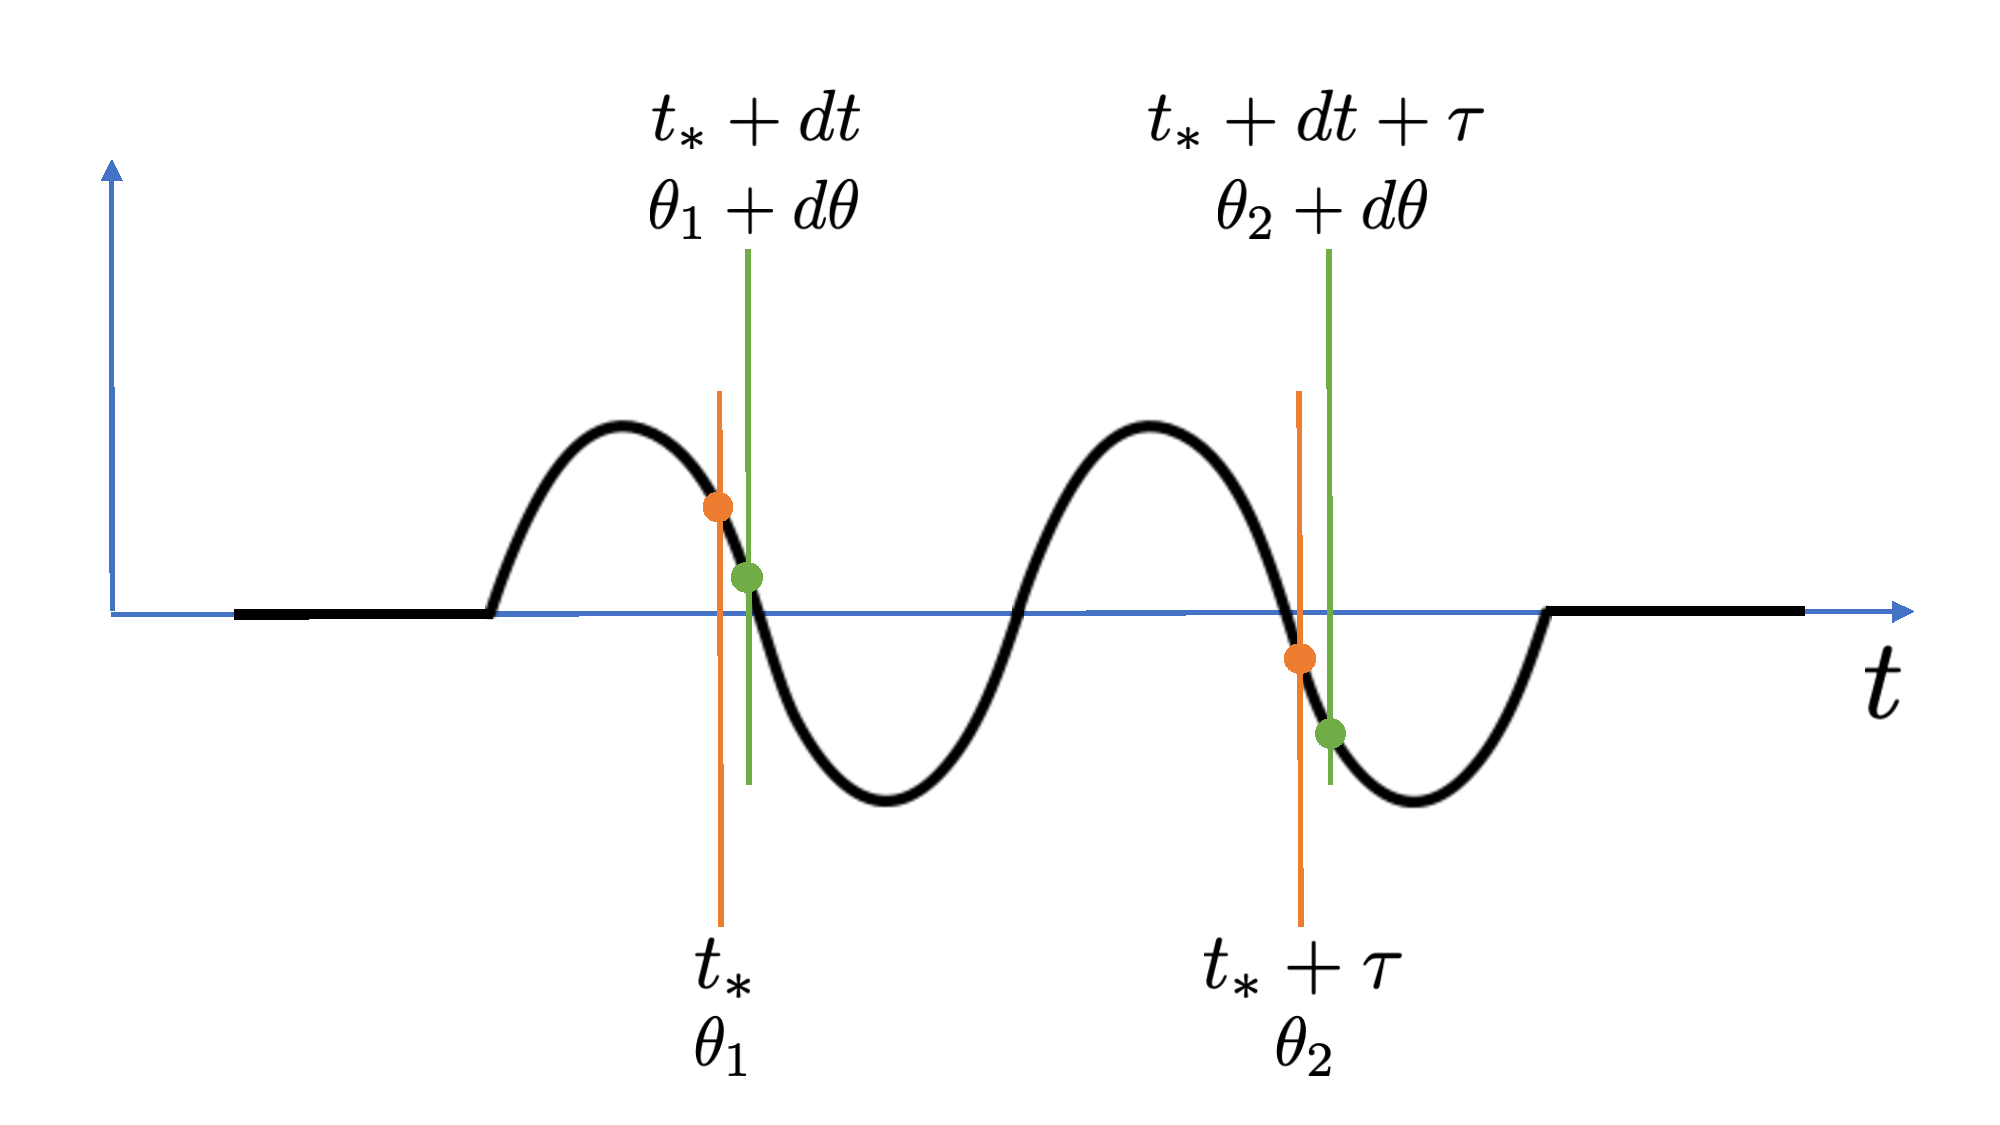
\includegraphics[width=.7\textwidth]{../../images/temp_cohe_1.pdf}
    \caption{}
    \label{fig:laser_temp_cohe}
\end{figure}

\begin{figure}
    \centering
    \begin{subfigure}{.7\textwidth}
      \centering
      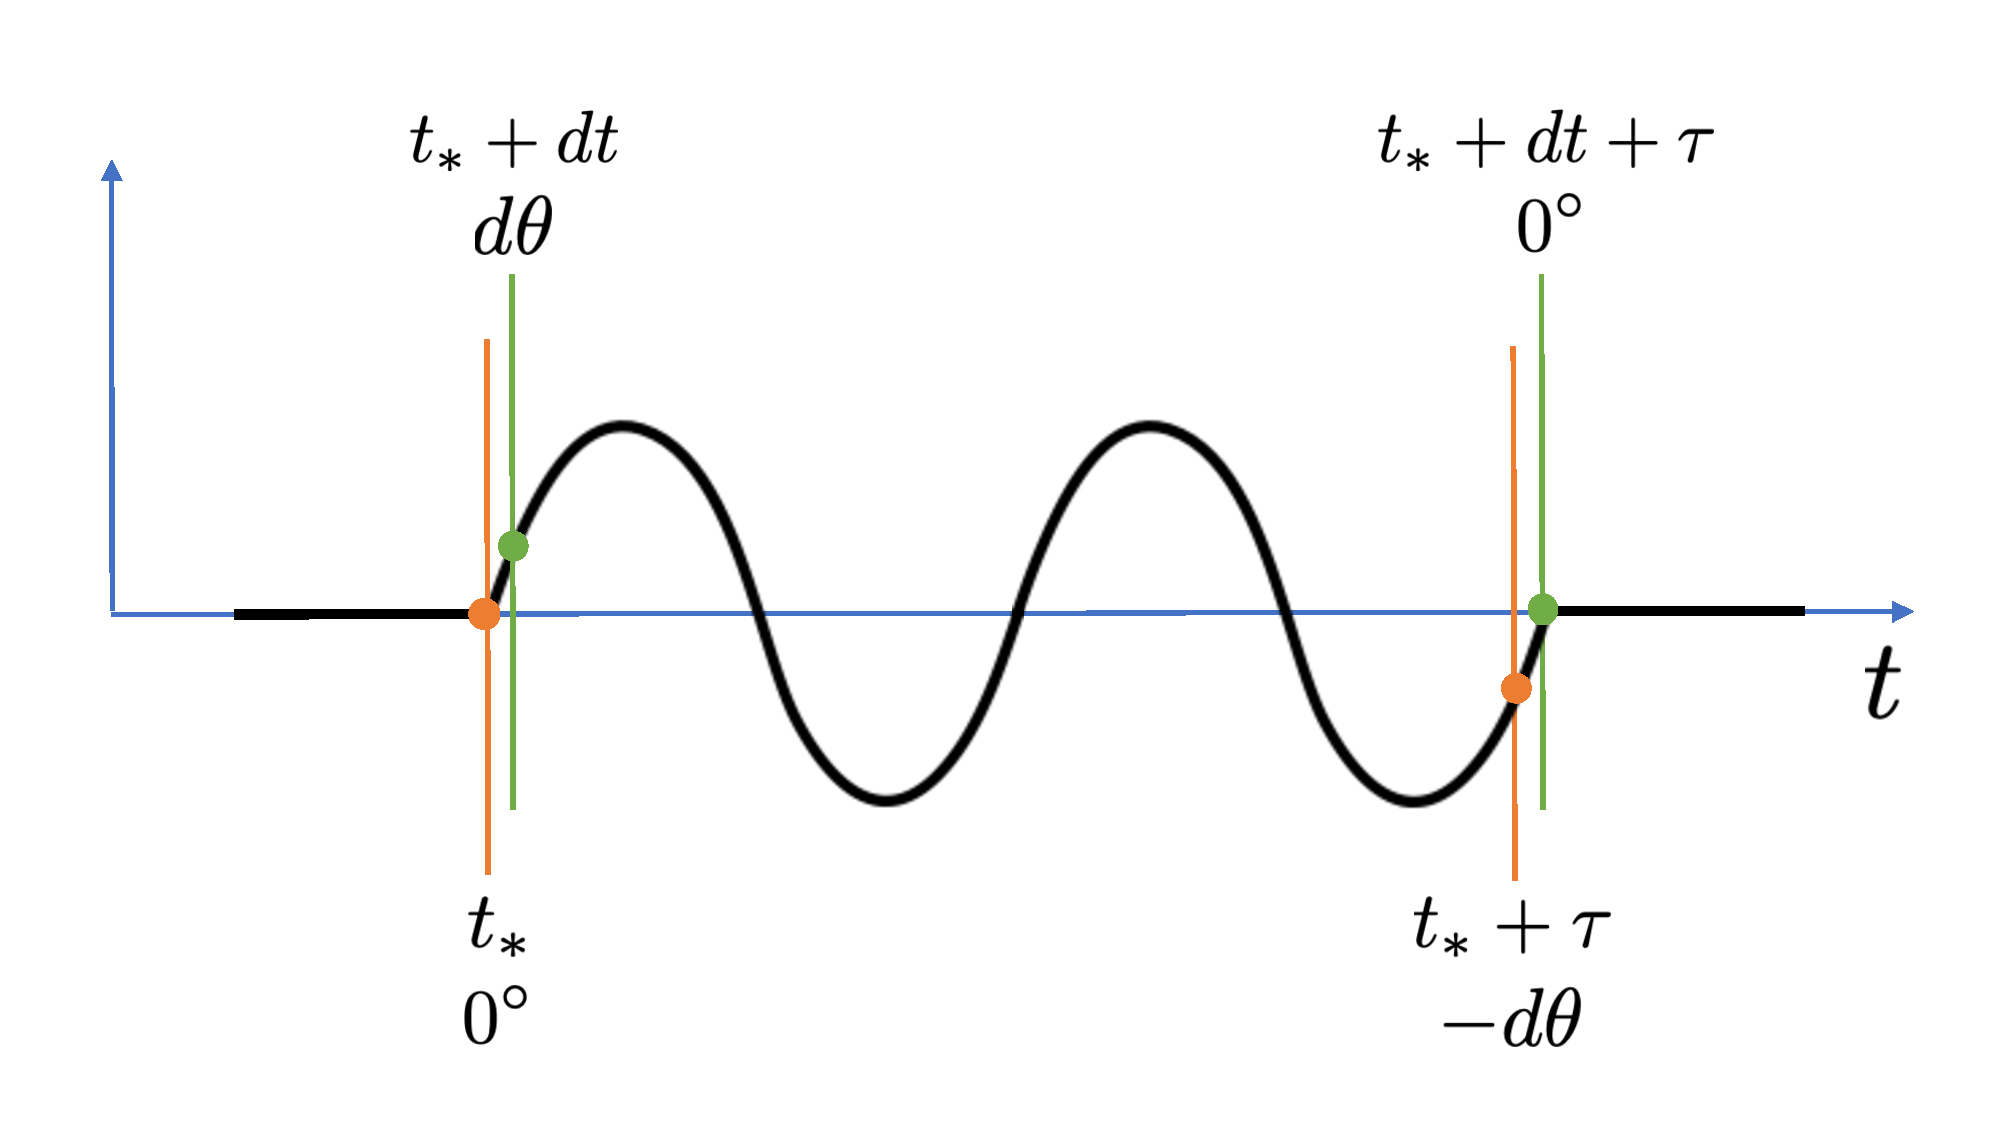
\includegraphics[width=\textwidth]{../../images/temp_cohe_2.pdf}
      \caption{}
      \label{fig:laser_temp_cohe_1}
    \end{subfigure}
    \begin{subfigure}{.7\textwidth}
        \centering
        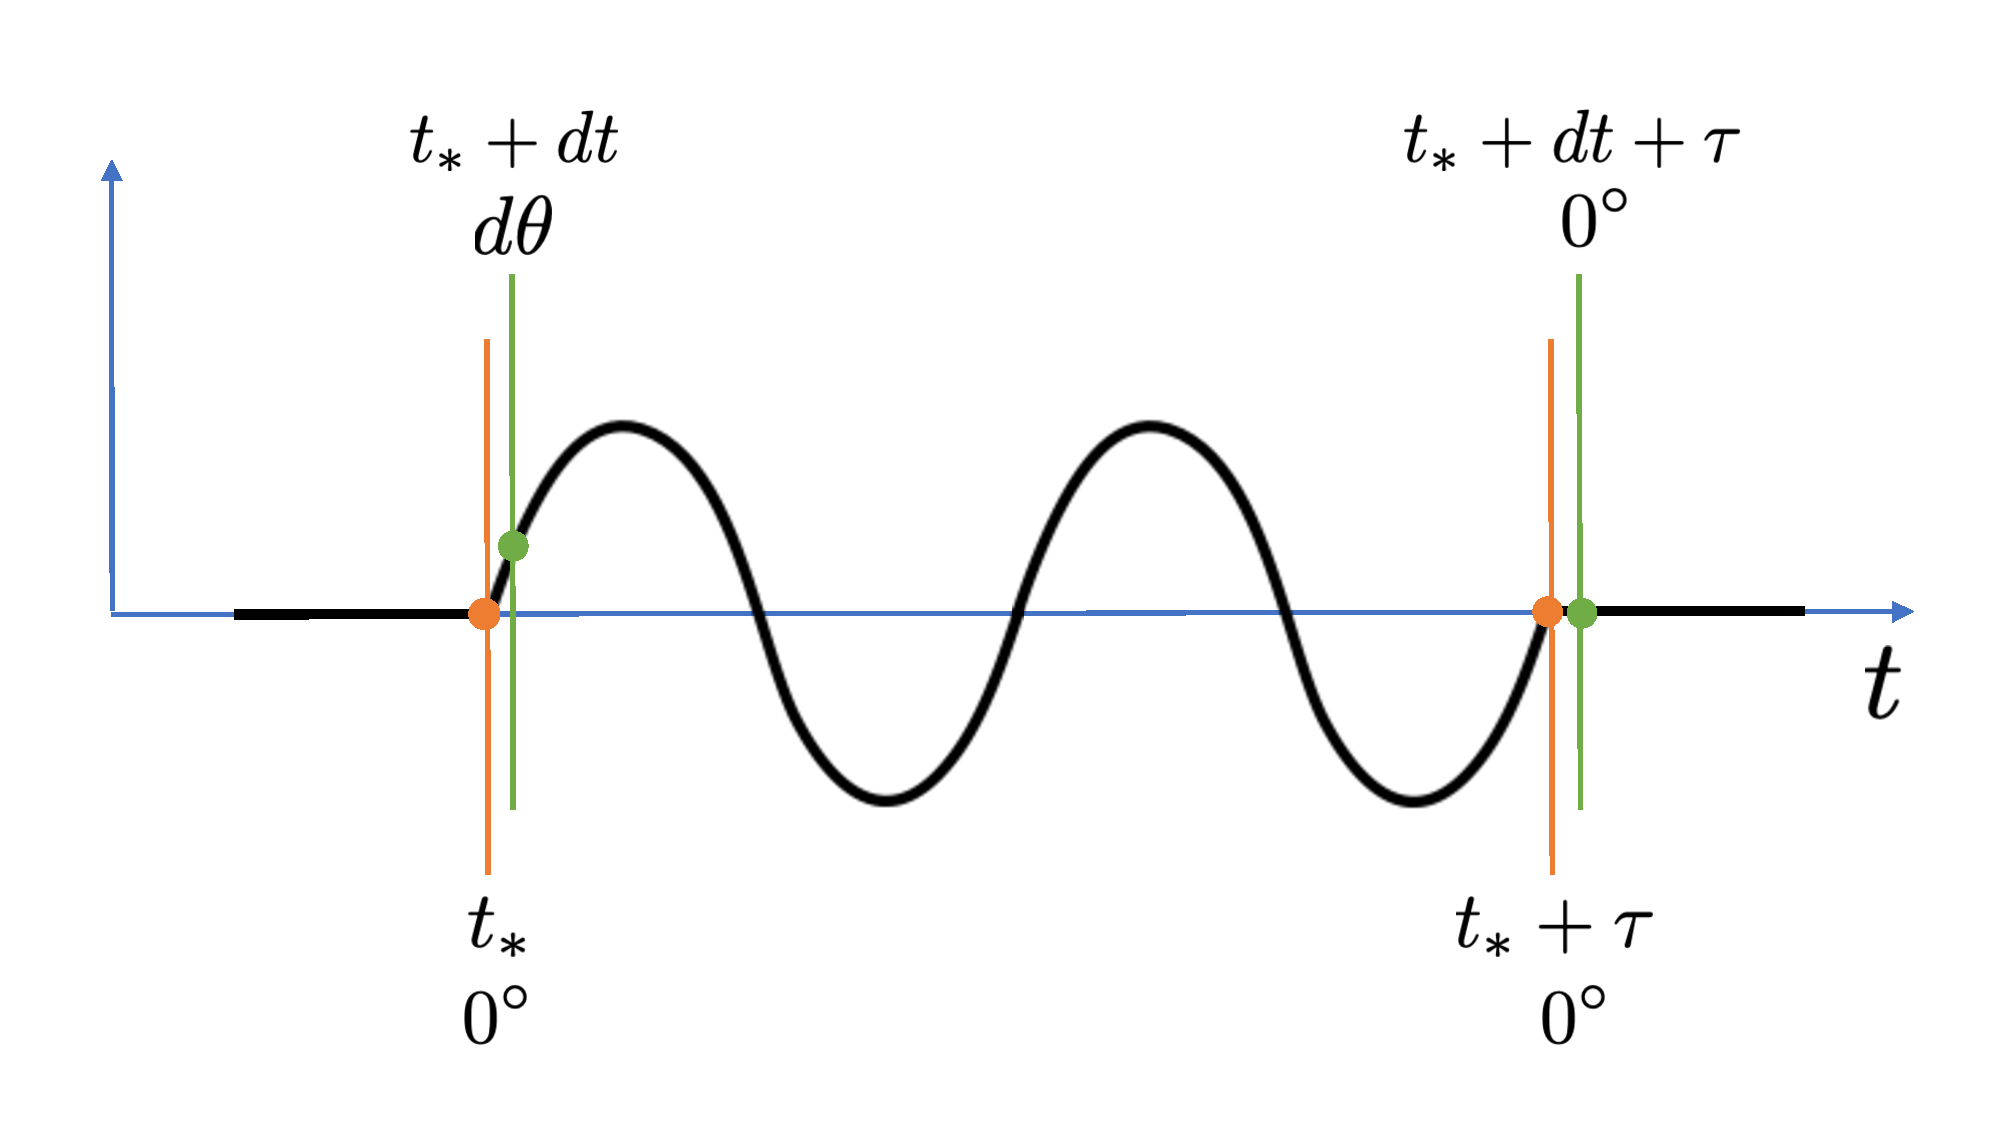
\includegraphics[width=\textwidth]{../../images/temp_cohe_3.pdf}
        \caption{}
        \label{fig:laser_temp_cohe_2}
      \end{subfigure}
    \caption{Depiction of temporal coherence for a light pulse.}
    \label{fig:laser_temp_cohe_12}
\end{figure}

A depiction of temporal coherence is provided in \cref{fig:laser_temp_cohe}, which shows a light pulse as a function of time. An arbitrary time $t_*$ is chosen along the light wave, and the wave's phase at that time is $\theta_1$. At the time $t_* + \tau$ the wave has a different phase $\theta_2$, and thus the phase difference between times $t_*$ and $t_*+\tau$ is $\theta_2 - \theta_1$. This is depicted by the orange dots. The green dots are used to highlight the phase difference between times $t_*+dt$ and $t_*+dt+\tau$. In this case, the phases are respectively $\theta_1 + d\theta$ and $\theta_2 + d\theta$, and hence the phase difference is still maintained at $\theta_2 - \theta_1$.

Rather than picking the time $t_*$ to be at an arbitrary location along the wave, in \cref{fig:laser_temp_cohe_1} we choose $t_*$ to be at the beginning of the wave, and also choose $\tau$ to be just a bit smaller than the entire duration of the pulse. For this case, the phase difference between $t_*$ and $t_*+\tau$ is $d\theta$, which is equal to the phase difference between $t_*+dt$ and $t_*+dt+\tau$. On the other hand, in \cref{fig:laser_temp_cohe_2} we have chosen $\tau$ to be just a bit larger so as to be equal to the duration of the wave. For this case the phase difference between $t_*$ and $t_*+\tau$ is zero, which is not the same as the phase difference between $t_*+dt$ and $t_*+dt+\tau$, namely $d\theta$. Thus, the maximum value of $\tau$ that maintains a constant phase difference has been reached, and therefore by definition this value is referred to as the temporal coherence length $\tau_c$ at time $t_*$ (other locations of $t_*$, such as that in \cref{fig:laser_temp_cohe}, have a different $\tau_c$).

%########################################################################
\chapter{Longitudinal and transverse waves}
%########################################################################

%------------------------------------------------------------------------
\section{Definitions}
%------------------------------------------------------------------------
The Helmholtz decomposition for a function $\Fvec = \Fvec(\xvec,t)$ is of the following form
\begin{equation}
    \Fvec = \Fvec_l + \Fvec_t,
\end{equation}
where $\Fvec_l = \Fvec_l(\xvec,t)$ is the longitudinal component and $\Fvec_t = \Fvec_t(\xvec,t)$ the transverse component. These are defined by
\begin{align}
    \nabla \times \Fvec_l &= 0, \label{eq:ltw_plasma_long_def}\\
    \nabla \cdot \Fvec_t &= 0. \label{eq:ltw_plasma_tran_def}
\end{align}
We'll assume that any vector function $\Gvec = \Gvec(\xvec,t)$ can be expressed as the real component of
\begin{equation}
    \label{eq:em_more_general_wave_form}
    \Gvec = \hat{\Gvec} \exp \left [ i \left ( \int_0^x k_x(x') \, dx' + \int_0^y k_y(y') \, dy' + \int_0^z k_z(z') \, dz'  - wt \right ) \right ].
\end{equation}
For the above, $w$ a frequency constant in time and space, and $k_x = k_x(x)$, $k_y = k_y(y)$, and $k_z = k_z(z)$ form the wave vector $\kvec = [k_x, k_y, k_z]$. $\hat{\Gvec} = \hat{\Gvec}(\xvec,t)$ is a complex vector where the real and complex components point in the same direction. Additionally, we enforce the constraint that if $\nabla \times \Gvec = 0$, then $\nabla \times \hat{\Gvec} = 0$, and similarly, if $\nabla \cdot \Gvec = 0$, then $\nabla \cdot \hat{\Gvec} = 0$. We'll often use a different subscript in the wave vectors and frequencies of different waves. For example, we'll use $\kvec_e$ for electron-plasma waves, $\kvec_i$ for ion-acoustic waves, $\kvec_L$ for laser waves, and $\kvec_s$ for scattered waves. Similarly for the frequencies $w_e$, $w_i$, $w_L$, $w_s$.

We note that
\begin{multline}
    \nabla \exp \left [ i \left ( \int_0^x k_x(x') \, dx' + \int_0^y k_y(y') \, dy' + \int_0^z k_z(z') \, dz'  - wt \right ) \right ] \\
    = i \kvec \exp \left [ i \left ( \int_0^x k_x(x') \, dx' + \int_0^y k_y(y') \, dy' + \int_0^z k_z(z') \, dz'  - wt \right ) \right ]
\end{multline}
Given the identity $\nabla \times (\Avec f) = (\nabla \times \Avec ) f - \Avec \times (\nabla f)$, we can show that
\begin{align}
    \label{eq:ltw_no_curl}
    \nabla \times \Gvec &= \nabla \times \left [ \hat{\Gvec} \exp (...) \right ] \nonumber \\
    &= \left ( \nabla \times \hat{\Gvec} \right ) \exp (...) - \hat{\Gvec} \times \left [ \nabla \exp (...) \right ] \nonumber \\
    &= \left ( \nabla \times \hat{\Gvec} \right ) \exp (...) - \hat{\Gvec} \times \left [ i\kvec \exp (...) \right ] \nonumber \\
    &= \left ( \nabla \times \hat{\Gvec} \right ) \exp (...) + i \kvec \times \Gvec.
\end{align}
Given the identity $\nabla \cdot (\Avec f) = ( \nabla \cdot \Avec) f + \Avec \cdot (\nabla f)$, we can show that
\begin{align}
    \label{eq:ltw_no_div}
    \nabla \cdot \Gvec &= \nabla \cdot \left [ \hat{\Gvec} \exp (...) \right ] \nonumber \\
    &= \left ( \nabla \cdot \hat{\Gvec} \right ) \exp (...) + \hat{\Gvec} \cdot \left [ \nabla \exp (...) \right ] \nonumber \\
    &= \left ( \nabla \cdot \hat{\Gvec} \right ) \exp (...) + \hat{\Gvec} \cdot \left [ i \kvec \exp (...) \right ] \nonumber \\
    &= \left ( \nabla \cdot \hat{\Gvec} \right ) \exp (...) + i \kvec \cdot \Gvec.
\end{align}
By definition, $\Fvec_l$ has no curl and $\Fvec_t$ has no divergence. As mentioned earlier, we then require $\hat{\Fvec}_l$ to have no curl and $\hat{\Fvec}_t$ to have no divergence. Using this in \cref{eq:ltw_no_curl,eq:ltw_no_div} allow us to write
\begin{align}
    \kvec \times \Fvec_l = 0 \label{eq:ltw_plasma_long_wavevector} \\
    \kvec \cdot \Fvec_t = 0 \label{eq:ltw_plasma_trans_wavevector}.
\end{align}

The first expression above says $\Fvec_l$ is parallel to $\kvec$ and the second says $\Fvec_t$ is orthogonal to $\kvec$. Thus, $\Fvec_l \cdot \Fvec_t = 0$. We will often have situations where $\nabla \times \Fvec = \nabla \cdot \Fvec = 0$, which by its own does not imply $\Fvec = 0$. However, using \cref{eq:ltw_no_curl,eq:ltw_no_div}, this translates to to $\kvec \times \Fvec = \kvec \cdot \Fvec =  0$. The latter equality states that $\kvec$ and $\Fvec$ are orthogonal, that is, the angle between them is $90^\circ$. The former equality leads to $|\Fvec| \sin(90^\circ) = 0$, which in turn means $\Fvec = 0$. To summarize,
\begin{equation}
    \label{eq:ltw_general_null_vector}
    \nabla \times \Fvec = \nabla \cdot \Fvec = 0 \to \Fvec = 0.
\end{equation}

For some cases we'll further restrict $\hat{\Gvec}$ in \cref{eq:em_more_general_wave_form} such that $\hat{\Gvec} = \hat{\Gvec} (\xvec)$, that is, the time dependence of the wave is fully captured by the $\exp(-iwt)$ term. For this case, we'll often re-write the expression for $\Gvec$ as
\begin{equation}
    \label{eq:em_semi_general_wave_form}
    \Gvec = \tilde{\Gvec} \exp (-iwt),
\end{equation}
where $\tilde{\Gvec} = \tilde{\Gvec}(\xvec)$ is given by
\begin{equation}
    \tilde{\Gvec} = \hat{\Gvec} \exp \left [ i \left ( \int_0^x k_x(x') \, dx' + \int_0^y k_y(y') \, dy' + \int_0^z k_z(z') \, dz' \right ) \right ].
\end{equation}
Finally, a further simplification occurs when $\kvec$ and $\hat{\Gvec}$ are assumed to be constant in space. For this case, the expression for $\Gvec$ becomes
\begin{equation}
    \label{eq:em_general_wave_form}
    \Gvec = \hat{\Gvec} \exp \left [i\left ( \kvec \cdot \xvec - wt \right ) \right ].
\end{equation}
These are the so-called plane waves. We end with the cautionary note that the second gradients of $\Gvec$ in \cref{eq:em_more_general_wave_form} are not necessarily the same as those of $\Gvec$ in \cref{eq:em_general_wave_form}.

%------------------------------------------------------------------------
\section{Electron-plasma and ion-acoustic waves}
%------------------------------------------------------------------------
For both electron-plasma and ion-acoustic waves we can assume the magnetic field does not change. Thus, Faraday's law gives
\begin{equation}
    \nabla \times \Evec = \nabla \times \Evec_t = 0.
\end{equation}
By definition, $\nabla \cdot \Evec_t = 0$. Thus, using \cref{eq:ltw_general_null_vector} we get $\Evec_t = 0$, that is, $\Evec = \Evec_l$. 

For electron-plasma waves, we can use \cref{eq:em_general_wave_form} to write \cref{eq:ep_waves_mom_linearized} in spectral form and thus obtain
\begin{equation}
-i w n_{e0} \hat{\uvec}_{e1} + \frac{e n_{e0}}{m_e} \hat{\Evec}_{1,l} = -\kvec_e \frac{\gamma_e p_{e0}}{n_{e0} m_e} \hat{n}_{e1}. 
\end{equation}
Since the second term on the left-hand side and the term on the right-hand side point along $\kvec_e$, $\hat{\uvec}_{e1}$ also points along $\kvec_e$, that is, $\hat{\uvec}_{e1} = \hat{\uvec}_{e1,l}$.

For ion-acoustic waves, we can use \cref{eq:em_general_wave_form} to write \cref{eq:ia_waves_mom_linearized} in spectral form and thus obtain
\begin{equation}
-i w n_{i0} \hat{\uvec}_{i1} - \frac{Z e n_{i0}}{m_i} \hat{\Evec}_{1,l} = -\kvec_i \frac{\gamma_i p_{i0}}{n_{i0} m_i} \hat{n}_{i1}. 
\end{equation}
Since the second term on the left-hand side and the term on the right-hand side point along $\kvec_i$, $\hat{\uvec}_{i1}$ also points along $\kvec_i$, that is, $\hat{\uvec}_{i1} = \hat{\uvec}_{i1,l}$. Finally, we note that the electric field being purely longitudinal is in agreement with \cref{eq:ia_waves_E}.

%########################################################################
\chapter{Electromagnetic waves in plasmas}
%########################################################################

\label{sec:electromagnetic_waves_plasmas}
In introductory electrodynamics, one typically studies electromagnetic waves in vacuum, that is, for cases where $\rho_q = \Jvec = 0$. In this section we relax both of these assumptions. Consider the electric and magnetic fields as well as the scalar and vector potentials, which satisfy
\begin{equation}
    \label{eq:emp_general_E_potential}
    \Evec = -\nabla \phi - \frac{\partial \Avec}{\partial t},
\end{equation}
\begin{equation}
    \label{eq:emp_general_B_potential}
    \Bvec = \nabla \times \Avec.
\end{equation}
For the above, we choose $\nabla \cdot \Avec = 0$. Using the fact that the magnetic field is solenoidal, we have
\begin{equation*}
    \nabla \cdot \Bvec = \nabla \cdot \Bvec_l + \nabla \cdot \Bvec_t = \nabla \cdot \Bvec_l = 0.
\end{equation*}
However, by definition, $\nabla \times \Bvec_l = 0$ as well. Thus, using \cref{eq:ltw_general_null_vector}, we have $\Bvec_l = 0$. The same argument applies to the vector potential, and thus $\Avec_l = 0$. For the electric field, we have
\begin{equation*}
    \nabla \cdot \Evec = \nabla \cdot \Evec_l + \nabla \cdot \Evec_t = \nabla \cdot \Evec_l .
\end{equation*}
Taking the divergence of \cref{eq:emp_general_E_potential}, we get
\begin{equation}
    \nabla \cdot \Evec = \nabla \cdot \left ( -\nabla \phi \right ).
\end{equation}
Combining the last two equations gives
\begin{equation*}
    \nabla \cdot \left ( \Evec_l + \nabla \phi \right ) = 0.
\end{equation*}
By definition, we also have
\begin{equation*}
    \nabla \times \left ( \Evec_l + \nabla \phi \right ) = 0.
\end{equation*}
Thus, using \cref{eq:ltw_general_null_vector}, we have $\Evec_l = -\nabla \phi$. A similar argument can be used to show $\Evec_t = -\partial \Avec / \partial t$. Our goal in this section will be to determine equations for $\Evec_l$, $\Evec_t$ and $\Bvec$.

We'll begin with the conservation of charge equation
\begin{equation*}
    \frac{\partial \rho_q}{\partial t} + \nabla \cdot \Jvec = 0,
\end{equation*}
which we re-write as
\begin{equation*}
    \frac{\partial \rho_q}{\partial t} + \nabla \cdot \Jvec_l = 0,
\end{equation*}
Using Poisson's equation $\nabla^2\phi = -\rho_q / \epsilon_0$ in the above, we get
\begin{equation*}
    \frac{\partial}{\partial t} \left ( -\epsilon_0 \nabla^2 \phi \right ) + \nabla \cdot \Jvec_l = 0,
\end{equation*}
or
\begin{equation*}
    \nabla \cdot \left ( \frac{\partial \nabla \phi}{\partial t} - \frac{1}{\epsilon_0} \Jvec_l \right ) = 0.
\end{equation*}
However, by definition, we also have
\begin{equation*}
    \nabla \times \left ( \frac{\partial \nabla \phi}{\partial t} - \frac{1}{\epsilon_0} \Jvec_l \right ) = 0.
\end{equation*}
Using \cref{eq:ltw_general_null_vector}, we conclude
\begin{equation}
    \label{eq:emp_general_longitudinal_J}
    \frac{\partial \nabla \phi}{\partial t} = \frac{1}{\epsilon_0} \Jvec_l.
\end{equation}
This gives the equation for $\Evec_l$, namely,
\begin{equation}
    \label{eq:emp_general_long_E}
    \frac{\partial^2 \Evec_l}{\partial t^2} + \frac{1}{\epsilon_0} \frac{\partial \Jvec_l}{\partial t} = 0.
\end{equation}

Both $\Evec_t$ and $\Bvec$ can be extracted from $\Avec$, so now we proceed to find an equation for the transverse vector potential. Ampere's law with Maxwell's correction gives
\begin{equation*}
    \nabla \times \left ( \nabla \times \Avec \right ) = \mu_0 \Jvec + \mu_0 \epsilon_0 \frac{\partial \Evec}{\partial t}.
\end{equation*}
The above is re-written as
\begin{equation*}
    \nabla \left ( \nabla \cdot \Avec \right ) - \nabla^2 \Avec = \mu_0 \Jvec + \mu_0 \epsilon_0 \left ( -\frac{\partial \nabla \phi}{\partial t} - \frac{\partial^2 \Avec}{\partial t^2} \right ),
\end{equation*}
which gives
\begin{equation*}
    \frac{\partial^2 \Avec}{\partial t} - \frac{1}{\mu_0 \epsilon_0} \nabla^2 \Avec = \frac{1}{\epsilon_0} \Jvec - \frac{\partial \nabla \phi}{\partial t},
\end{equation*}
or
\begin{equation*}
    \frac{\partial^2 \Avec}{\partial t} - c_0^2 \nabla^2 \Avec = \frac{1}{\epsilon_0} \Jvec - \frac{\partial \nabla \phi}{\partial t},
\end{equation*}
where $c_0 = 1/\sqrt{\mu_0 \epsilon_0}$. Expanding the current density as $\Jvec = \Jvec_l + \Jvec_t$, and using \cref{eq:emp_general_longitudinal_J}, we get
\begin{equation}
    \label{eq:emp_general_trans_vec_pot}
    \frac{\partial^2 \Avec}{\partial t} - c_0^2 \nabla^2 \Avec = \frac{1}{\epsilon_0} \Jvec_t.
\end{equation}
Using the functional form in \cref{eq:em_general_wave_form} for $\Avec$ and $\Jvec_t$ gives
\begin{equation}
    -w^2 \hat{\Avec} + k^2 c_0^2 \hat{\Avec}= \frac{1}{\epsilon_0} \hat{\Jvec}_t.
\end{equation}
That is, $\Avec$ and $\Jvec_t$ point in the same direction.

Taking the time derivative of \cref{eq:emp_general_trans_vec_pot} gives the equation for $\Evec_t$, that is
\begin{equation}
    \label{eq:emp_general_trans_E}
    \frac{\partial^2 \Evec_t}{\partial t^2} - c_0^2 \nabla^2 \Evec_t + \frac{1}{\epsilon_0} \frac{\partial \Jvec_t}{\partial t} = 0.
\end{equation}
Taking the curl of \cref{eq:emp_general_trans_vec_pot} gives the equation for $\Bvec$, that is
\begin{equation}
    \label{eq:emp_general_trans_B}
    \frac{\partial^2 \Bvec}{\partial t^2} - c_0^2 \nabla^2 \Bvec - \frac{1}{\epsilon_0} \nabla \times \Jvec_t = 0.
\end{equation}
Using the functional form in \cref{eq:em_general_wave_form} for $\Evec_t$, $\Bvec$ and $\Jvec_t$ gives
\begin{equation}
    -w^2 \hat{\Evec}_t + k^2 c_0^2 \hat{\Evec}_t - \frac{iw}{\epsilon_0} \hat{\Jvec}_t = 0,
\end{equation}
\begin{equation}
    -w^2 \Bvec + k^2 c_0^2 \Bvec - \frac{i}{\epsilon_0} \kvec \times \Jvec_t = 0.
\end{equation}
That is, $\Evec_t$ points in the same direction as $\Jvec_t$, which as shown before points in the same direction as $\Avec$. Additionally, $\Bvec$ points in the direction of $\kvec \times \Jvec_t$, that is, it is orthogonal to $\Evec_t$.

We briefly note that taking the curl of \cref{eq:p_waves_maxwell_1}, and using \cref{eq:p_waves_maxwell_2}, gives the wave equation for the total electric field $\Evec$, that is 
\begin{equation}
    \frac{\partial^2 \Evec}{\partial t^2} - c_0^2 \nabla^2 \Evec + c_0^2 \nabla (\nabla \cdot \Evec) + \frac{1}{\epsilon_0} \frac{\partial \Jvec}{\partial t} = 0.
\end{equation}
The above can be considered as the sum of the following three equations
\begin{align*}
    \frac{\partial^2 \Evec_l}{\partial t^2} + \frac{1}{\epsilon_0} \frac{\partial \Jvec_l}{\partial t} &= 0, \\
    \frac{\partial^2 \Evec_t}{\partial t^2} - c_0^2 \nabla^2 \Evec_t + \frac{1}{\epsilon_0} \frac{\partial \Jvec_t}{\partial t} &= 0, \\
    -c_0^2 \nabla^2 \Evec_l + c_0^2 \nabla (\nabla \cdot \Evec_l) &= 0.
\end{align*}
The first is the equation for the longitudinal electric field, that is \cref{eq:emp_general_long_E}. The second is the equation for the transverse electric field, that is \cref{eq:emp_general_trans_E}. The third equation above follows from the vector identity $\nabla \times (\nabla \times \Fvec) = -\nabla^2 \Fvec + \nabla ( \nabla \cdot \Fvec )$ and the fact that $\nabla \times \Evec_l = 0$.

It will often be the case that transverse waves will oscillate at such a fast rate that the ions, which have a large inertia, will be unable to react quickly enough. Thus, we can assume $\uvec_{i,t} = 0$. Given the definition of the current density in \cref{eq:p_waves_curr_density}, the transverse current density is expressed as $\Jvec_t = e \left (Z n_i \uvec_{i,t} - n_e \uvec_{e,t} \right )$, which now simplifies to 
\begin{equation}
    \label{eq:emp_transverse_current}
    \Jvec_t = -e n_e \uvec_{e,t}.
\end{equation}
Thus, the transverse electron velocity $\uvec_{e,t}$ points in the same direction as $\Jvec_t$, which is the same direction as $\Evec_t$ and $\Avec$. The next section focuses on deriving an expression for $\uvec_{e,t}$. 

We begin with \cref{eq:pwaves_electron_momentum}, the electron momentum equation, which, due to the electron continuity equation, can be written as
\begin{equation*}
    m_e n_e \frac{\partial\uvec_e}{\partial t} + m_e n_e \uvec_e \cdot \nabla \uvec_e + e n_e \left ( \Evec + \uvec_e \times \Bvec \right ) = -\nabla p_e,
\end{equation*}
or
\begin{equation*}
    \frac{\partial\uvec_e}{\partial t} + \uvec_e \cdot \nabla \uvec_e + \frac{e}{m_e} \left ( \Evec + \uvec_e \times \Bvec \right ) = -\frac{1}{n_e m_e}\nabla p_e,
\end{equation*}
Using the scalar and vector potentials we have
\begin{equation*}
    \frac{\partial\uvec_e}{\partial t} + \uvec_e \cdot \nabla \uvec_e +\frac{e}{m_e} \left [ -\nabla \phi - \frac{\partial \Avec}{\partial t} + \uvec_e \times \left ( \nabla \times \Avec \right ) \right ] = -\frac{1}{n_e m_e} \nabla p_e.
\end{equation*}
Using the vector identity $\nabla \left ( F^2 / 2 \right ) = \Fvec \times \left ( \nabla \times \Fvec \right ) + \Fvec \cdot \nabla \Fvec$, we write the above as
\begin{equation}
    \frac{\partial\uvec_e}{\partial t} - \uvec_e \times \left ( \nabla \times \uvec_e \right ) + \nabla \left (\frac{u_e^2}{2} \right ) + \frac{e}{m_e} \left [ -\nabla \phi - \frac{\partial \Avec}{\partial t} + \uvec_e \times \left ( \nabla \times \Avec \right ) \right ] = -\frac{1}{n_e m_e} \nabla p_e,
\end{equation}
which is equivalent to 
\begin{equation}
    \label{eq:emp_electron_momentum}
    \frac{\partial\uvec_e}{\partial t} - \uvec_e \times \left ( \nabla \times \uvec_{e,t} \right ) + \nabla \left (\frac{u_e^2}{2} \right ) + \frac{e}{m_e} \left [ -\nabla \phi - \frac{\partial \Avec}{\partial t} + \uvec_e \times \left ( \nabla \times \Avec \right ) \right ] = -\frac{1}{n_e m_e} \nabla p_e.
\end{equation}
We'll now introduce a more specific coordinate system. We'll be dealing with at most three waves at a time: a laser wave, a scattered wave, and a plasma wave (either electron-plasma or ion-acoustic wave). We'll assume all three of these waves lie on a so-called base plane. That is, $\kvec_e$ (or $\kvec_i$), $\kvec_L$, and $\kvec_s$ all point along this plane. We now choose the main transverse direction, that is, the direction of $\uvec_{e,t}$, $\Jvec_t$, $\Evec_t$, and $\Avec$ to be the direction orthogonal to this plane, so that these vectors are orthogonal to any $\kvec$. As an aside, we note that the longitudinal and transverse components of the electron velocity can belong to different waves. That is
\begin{align}
    \uvec_{e,l} &= \hat{\uvec}_{e,l} \exp \left [ i (\kvec_p \cdot \xvec - w_pt) \right ] \\
    \uvec_{e,t} &= \hat{\uvec}_{e,t} \exp \left [ i (\kvec_q \cdot \xvec - w_qt) \right ].
\end{align}
The vectors $\nabla \left ( u_e^2 / 2 \right )$, $\nabla \phi$ and $\nabla p_e$ are all by definition longitudinal. As \cref{eq:ltw_plasma_long_wavevector} states, longitudinal vectors point along their wave vectors. Since we chose all wave vectors to be confined to the base plane, $\nabla \left ( u_e^2 / 2 \right )$, $\nabla \phi$ and $\nabla p_e$ do not have a component along the main transverse direction. As a result, the component of \cref{eq:emp_electron_momentum} along the main transverse direction simplifies to
\begin{equation}
    \label{eq:emp_electron_momentum_transverse}
    \frac{\partial\uvec_{e,t}}{\partial t} - \uvec_{e,l} \times \left ( \nabla \times \uvec_{e,t} \right ) + \frac{e}{m_e} \left [ - \frac{\partial \Avec}{\partial t} + \uvec_{e,l} \times \left ( \nabla \times \Avec \right ) \right ] = 0.
\end{equation}
Using $c = w/k$, we show the following scalings 
\begin{align}
    \frac{1}{c^2} \frac{\partial \uvec_{e,t}}{\partial t} &= -\frac{iw \uvec_{e,t}}{c^2} \sim i \frac{\uvec_{e,t}}{c} k , \nonumber \\
    \frac{1}{c^2} \uvec_{e,l} \times \left (\nabla \times \uvec_{e,t} \right ) & = \frac{i \uvec_{e,l} \times \left ( \kvec \times \uvec_{e,t} \right ) }{c^2} \sim i \frac{\uvec_{e,l}}{c} \frac{\uvec_{e,t}}{c} k , \nonumber \\
    \frac{1}{c^2} \frac{\partial \Avec}{\partial t} &= -\frac{iw \Avec}{c^2} \sim i \frac{\Avec}{c} k , \nonumber \\
    \frac{1}{c^2} \uvec_{e,l} \times \left ( \nabla \times \Avec \right ) &= \frac{i \uvec_{e,l} \times \left ( \kvec \times \Avec \right )}{c^2} \sim i \frac{\uvec_{e,l}}{c} \frac{\Avec}{c} k .
\end{align}
Thus, assuming $\uvec_{e,l} \ll c$, the terms involving the double cross product are smaller than those involving the time derivative. As a result, \cref{eq:emp_electron_momentum_transverse} becomes
\begin{equation}
    \frac{\partial\uvec_{e,t}}{\partial t} - \frac{e}{m_e} \frac{\partial \Avec}{\partial t} = 0.
\end{equation}
Using \cref{eq:em_semi_general_wave_form}, the above is equivalent to 
\begin{equation}
    -i w \uvec_{e,t} +i w \frac{e \Avec}{m_e} = 0,
\end{equation}
which upon re-arranging gives
\begin{equation}
    \label{eq:emp_transverse_velocity}
    \uvec_{e,t} = \frac{e\Avec}{m_e}.
\end{equation}

Using both the transverse current given by \cref{eq:emp_transverse_current} and the transverse velocity given by \cref{eq:emp_transverse_velocity}, \cref{eq:emp_general_trans_vec_pot} can be re-written as
\begin{equation*}
    \frac{\partial^2 \Avec}{\partial t} - c_0^2 \nabla^2 \Avec = -\frac{e n_e}{\epsilon_0} \uvec_{e,t} = -\frac{e^2 n_e}{\epsilon_0 m_e} \Avec.
\end{equation*}
We now use the decomposition $n_e = n_{e0} + n_{e1}$, where $n_{e0}$ is time independent. The above becomes
\begin{equation}
    \label{eq:emp_general_trans_vec_pot_complete}
    \frac{\partial^2 \Avec}{\partial t} + w_{pe}^2 \Avec - c_0^2 \nabla^2 \Avec = -\frac{e^2 n_{e1}}{\epsilon_0 m_e} \Avec,
\end{equation}
where $w_{pe}^2 = e^2 n_{e0} / m_e \epsilon_0$.

%########################################################################
\chapter{Electromagnetic waves in a stable plasma}
%########################################################################

%------------------------------------------------------------------------
\section{The vector potential}
%------------------------------------------------------------------------
\label{sec:semp_vector_potential}
We start with \cref{eq:emp_general_trans_vec_pot_complete}, but focus on the stable-plasma case, that is, $n_{e1} = 0$. Thus, we have
\begin{equation}
    \label{eq:semp_general_trans_vec_pot_complete}
    \frac{\partial^2 \Avec}{\partial t} + w_{pe}^2 \Avec - c_0^2 \nabla^2 \Avec = 0.
\end{equation}
We note that $n_{e0}$ is only time independent, that is, it is still allowed to vary across space. As a result, $w_{pe}^2$ is also allowed to vary across space. Using \cref{eq:em_semi_general_wave_form} for the vector potential, \cref{eq:semp_general_trans_vec_pot_complete} becomes
\begin{equation*}
    -w^2 \Avec + w_{pe}^2 \Avec - c_0^2 \nabla^2 \Avec = 0.
\end{equation*}
We re-write the above as
\begin{equation*}
    \frac{w^2}{c_0^2} \Avec - \frac{w^2}{c_0^2} \frac{w_{pe}^2}{w^2} \Avec + \nabla^2 \Avec = 0.
\end{equation*}
Defining $\epsilon = 1 - w_{pe}^2 / w^2$, we ultimately get
\begin{equation}
    \label{eq:semp_general_trans_vec_pot_complete_spec}
    \frac{w^2}{c_0^2} \epsilon \Avec + \nabla^2 \Avec = 0.
\end{equation}

We now consider the case of a \textit{uniform} stable plasma, that is, a plasma where $n_{e0}$ is uniform across space, and thus $w_{pe}$ and $\epsilon$ are also uniform across space. Using the standard plane-wave expression $\Avec = \hat{\Avec} \exp[i (\kvec \cdot \xvec - wt)]$ in \cref{eq:semp_general_trans_vec_pot_complete_spec} gives the following dispersion relation
\begin{equation}
    \label{eq:semp_uniform_dispersion_relation}
    \frac{w^2}{c_0^2} \epsilon = k^2.
\end{equation}
We expand the above to obtain
\begin{equation*}
    w^2 - w_{pe}^2 = c_0^2 k^2.
\end{equation*}
Taking the derivative $\partial / \partial k$ on both sides we get
\begin{equation*}
    2w \frac{\partial w}{\partial k} = 2 c_0^2 k,
\end{equation*}
which in turn gives the following expressions for the group velocity $v_g$
\begin{equation}
    v_g = \frac{c_0^2 k}{w}.
\end{equation}
Using \cref{eq:semp_uniform_dispersion_relation}, we can also write the above as
\begin{equation}
    v_g = \frac{c_0^2 k}{w} = c_0^2 \frac{\sqrt{\epsilon}}{c_0} = c_0 \sqrt{\epsilon}.
\end{equation}

%------------------------------------------------------------------------
\section{The electric field}
%------------------------------------------------------------------------
Taking the time derivative of \cref{eq:semp_general_trans_vec_pot_complete} gives the equation for $\Evec_t$, that is
\begin{equation}
    \label{eq:semp_general_trans_E_complete}
    \frac{\partial^2 \Evec_t}{\partial t^2} + w_{pe}^2 \Evec_t - c_0^2 \nabla^2 \Evec_t = 0.
\end{equation}
Using \cref{eq:em_semi_general_wave_form} for the electric field, the time derivative in \cref{eq:semp_general_trans_E_complete} evaluates such that 
\begin{equation*}
    -w^2 \Evec_t + w_{pe}^2 \Evec_t - c_0^2 \nabla^2 \Evec_t = 0.
\end{equation*}
We re-write the above as 
\begin{equation*}
    \frac{w^2}{c_0^2} \Evec_t - \frac{w^2}{c_0^2} \frac{w_{pe}^2}{w^2} \Evec_t + \nabla^2 \Evec_t = 0,
\end{equation*}
which becomes
\begin{equation}
    \label{eq:semp_general_trans_E_complete_spec}
    \frac{w^2}{c_0^2} \epsilon \Evec_t + \nabla^2 \Evec_t = 0.
\end{equation}

%------------------------------------------------------------------------
\section{The magnetic field}
%------------------------------------------------------------------------
Taking the curl of \cref{eq:semp_general_trans_vec_pot_complete} gives the equation for $\Bvec$, that is
\begin{equation}
    \label{eq:semp_general_trans_B_complete}
    \frac{\partial^2 \Bvec}{\partial t^2} + w_{pe}^2 \Bvec - c_0^2 \nabla^2 \Bvec + \nabla w_{pe}^2 \times \Avec = 0.
\end{equation}
Using \cref{eq:em_semi_general_wave_form} for the magnetic field, the time derivative in \cref{eq:semp_general_trans_B_complete} evaluates such that 
\begin{equation*}
    -w^2 \Bvec + w_{pe}^2 \Bvec - c_0^2 \nabla^2 \Bvec + \nabla w_{pe}^2 \times \Avec = 0.
\end{equation*}
We re-write the above as
\begin{equation*}
    \frac{w^2}{c_0^2} \Bvec - \frac{w^2}{c_0^2} \frac{w_{pe}^2}{w^2} \Bvec + \nabla^2 \Bvec - \frac{w^2}{c_0^2} \nabla \left ( \frac{w_{pe}^2}{w^2} \right ) \times \Avec = 0,
\end{equation*}
which becomes
\begin{equation*}
    \frac{w^2}{c_0^2} \epsilon \Bvec + \nabla^2 \Bvec + \frac{w^2}{c_0^2} \nabla \epsilon \times \Avec = 0.
\end{equation*}
Using \cref{eq:semp_general_trans_vec_pot_complete_spec} we get 
\begin{equation*}
    \frac{w^2}{c_0^2} \epsilon \Bvec + \nabla^2 \Bvec - \frac{1}{\epsilon} \nabla \epsilon \times \nabla^2 \Avec = 0.
\end{equation*}
The vector identity $\nabla \times \left ( \nabla \times \Fvec \right ) = \nabla \left ( \nabla \cdot \Fvec \right ) - \nabla^2 \Fvec$ gives $\nabla \times \left ( \nabla \times \Avec \right ) = -\nabla^2 \Avec $, or
\begin{equation}
    \label{eq:semp_b_to_a_vec_identity}
    \nabla \times \Bvec = -\nabla^2 \Avec.
\end{equation}
Thus, we finally get
\begin{equation}
    \label{eq:semp_general_trans_B_complete_spec}
    \frac{w^2}{c_0^2} \epsilon \Bvec + \nabla^2 \Bvec + \frac{1}{\epsilon} \nabla \epsilon \times \left ( \nabla \times \Bvec \right ) = 0.
\end{equation}

As a side note, we can use the expressions above to write Ampere's law in a new form. We combine the vector identity \cref{eq:semp_b_to_a_vec_identity} with \cref{eq:semp_general_trans_vec_pot_complete_spec} to obtain
\begin{equation*}
    \nabla \times \Bvec = \frac{w^2}{c_0^2} \epsilon \Avec.
\end{equation*}
Using \cref{eq:em_semi_general_wave_form} for the vector potential, the expression $\Evec_t = -\partial \Avec / \partial t$ gives
\begin{equation*}
    \Evec_t = iw \Avec.
\end{equation*}
Thus, the curl of $\Bvec$ can be expressed as
\begin{equation}
    \nabla \times \Bvec = -i \frac{w}{c_0^2} \epsilon \Evec_t.
\end{equation}

As mentioned in \cref{sec:semp_vector_potential}, for a uniform stable plasma we have $\epsilon$ equal to a constant. Thus, \cref{eq:semp_general_trans_B_complete_spec} becomes identical to \cref{eq:semp_general_trans_E_complete_spec}, that is, the wave forms of $\Evec_t$ and $\Bvec$ are the same. 

%########################################################################
\chapter{Stimulated Raman and Brillouin instabilities}
%########################################################################

%------------------------------------------------------------------------
\section{Linearization}
%------------------------------------------------------------------------
The following decompositions will be used in the derivation of stimulated Raman and Brillouin instabilities:
\begin{align}
    n_i &= n_{i0} + n_{i1}, \nonumber \\
    n_e &= n_{e0} + n_{e1}, \nonumber \\
    p_i &= p_{i0} + p_{i1}, \nonumber \\
    p_e &= p_{e0} + p_{e1}, \nonumber \\
    \uvec_{i,l} &= \uvec_{i0,l} + \uvec_{i1,l}, \nonumber \\
    \uvec_{e,l} &= \uvec_{e0,l} + \uvec_{e1,l}, \nonumber \\
    \Evec_l &= \Evec_{0,l} + \Evec_{1,l}, \nonumber \\
    \Avec &= \Avec_L + \Avec_s.
\end{align}
For these decompositions, we'll assume
\begin{enumerate}
    \item Terms with a subscript 1 are small and thus products of two small quantities can be neglected. \label{it:p_instabilities_assumption_1}
    \item $\uvec_{i0,l}$, $\uvec_{e0,l}$, and $\Evec_{0,l}$,are zero. \label{it:p_instabilities_assumption_2}
    \item $n_{i0}$, $n_{e0}$, $p_{i0}$, and $p_{e0}$ are uniform in space and time. \label{it:p_instabilities_assumption_3}
\end{enumerate}

Thus, unlike the previous section, we do not assume the plasma is stable, that is, we assume fluctuations such as $n_{e1}$ are small but non zero. $\Avec_L$ is the vector potential associated with the laser light, and $\Avec_s$ is the potential associated with the scattered light. For linearization purposes, we'll assume $\Avec_s$ is small. 

Using the decomposition for $\Avec$, \cref{eq:emp_general_trans_vec_pot_complete} is written as 
\begin{equation}
    \frac{\partial^2 \Avec_L}{\partial t} + \frac{\partial^2 \Avec_s}{\partial t} + w_{pe}^2 \Avec_L + w_{pe}^2 \Avec_s - c_0^2 \nabla^2 \Avec_L - c_0^2 \nabla^2 \Avec_s = -\frac{e^2 n_{e1}}{\epsilon_0 m_e} \Avec_L -\frac{e^2 n_{e1}}{\epsilon_0 m_e} \Avec_s,
\end{equation}
Dropping products of small quantities we have
\begin{equation}
    \label{eq:srs_temp1}
    \frac{\partial^2 \Avec_L}{\partial t} + \frac{\partial^2 \Avec_s}{\partial t} + w_{pe}^2 \Avec_L + w_{pe}^2 \Avec_s - c_0^2 \nabla^2 \Avec_L - c_0^2 \nabla^2 \Avec_s = -\frac{e^2 n_{e1}}{\epsilon_0 m_e} \Avec_L.
\end{equation}
We'll assume the laser light is stable, that is, it satisfies \cref{eq:semp_general_trans_vec_pot_complete}, which we re-write below
\begin{equation}
    \label{eq:srs_temp2}
    \frac{\partial^2 \Avec_L}{\partial t} + w_{pe}^2 \Avec_L - c_0^2 \nabla^2 \Avec_L = 0.
\end{equation}
Thus, \cref{eq:srs_temp1} becomes
\begin{equation}
    \frac{\partial^2 \Avec_s}{\partial t} + w_{pe}^2 \Avec_s - c_0^2 \nabla^2 \Avec_s = -\frac{e^2 n_{e1}}{\epsilon_0 m_e} \Avec_L.
\end{equation}
The above shows that the fluctuating $n_{e1}$ couples with the laser light to serve as a source for the scattered light.

The electron density equation is now written as
\begin{equation*}
    \frac{\partial n_{e0} + n_{e1}}{\partial t } + \nabla \cdot \left [ \left ( n_{e0} + n_{e1} \right )\left ( \uvec_{e,t} + \uvec_{e0,l} + \uvec_{e1,l} \right ) \right ] = 0,
\end{equation*}
which, since $\uvec_{e,t}$ is transverse, can be written as
\begin{equation*}
    \frac{\partial n_{e0} + n_{e1}}{\partial t } + \uvec_{e,t} \cdot \nabla \left (n_{e0} + n_{e1} \right ) + \nabla \cdot \left [ \left ( n_{e0} + n_{e1} \right )\left ( \uvec_{e0,l} + \uvec_{e1,l} \right ) \right ] = 0.
\end{equation*}
Given the assumptions in \cref{it:p_instabilities_assumption_1,it:p_instabilities_assumption_2,it:p_instabilities_assumption_3}, the above simplifies to
\begin{equation*}
    \frac{\partial n_{e1}}{\partial t } + \uvec_{e,t} \cdot \nabla n_{e1} + \nabla \cdot \left ( n_{e0} \uvec_{e1,l} \right ) = 0.
\end{equation*}
Since $\uvec_{e,t}$ and $\nabla n_{e1}$ are orthogonal, we finally have
\begin{equation}
    \label{eq:p_instabilities_e_den_linearized}
    \frac{\partial n_{e1}}{\partial t} + \nabla \cdot \left ( n_{e0} \uvec_{e1,l} \right ) = 0.
\end{equation}

The ion density equation is now written as
\begin{equation*}
    \frac{\partial n_{i0} + n_{i1}}{\partial t } + \nabla \cdot \left [ \left ( n_{i0} + n_{i1} \right )\left ( \uvec_{i,t} + \uvec_{i0,l} + \uvec_{i1,l} \right ) \right ] = 0,
\end{equation*}
As stated in \cref{sec:electromagnetic_waves_plasmas}, it is often the case that transverse waves oscillate at such a fast rate that the ions, which have large inertia, are unable to react on comparable time scales. Thus, we can assume $\uvec_{i,t} = 0$,
\begin{equation*}
    \frac{\partial n_{i0} + n_{i1}}{\partial t } + \nabla \cdot \left [ \left ( n_{i0} + n_{i1} \right )\left ( \uvec_{i0,l} + \uvec_{i1,l} \right ) \right ] = 0.
\end{equation*}
Given the assumptions in \cref{it:p_instabilities_assumption_1,it:p_instabilities_assumption_2,it:p_instabilities_assumption_3}, the above simplifies to
\begin{equation}
    \label{eq:p_instabilities_i_den_linearized}
    \frac{\partial n_{i1}}{\partial t } + \nabla \cdot \left ( n_{i0} \uvec_{i1,l} \right ) = 0.
\end{equation}

Consider the electron momentum equation. Subtracting \cref{eq:emp_electron_momentum_transverse} from \cref{eq:emp_electron_momentum} gives
\begin{equation}
    \label{eq:emp_electron_momentum_longitudinal}
    \frac{\partial\uvec_{e,l}}{\partial t} - \uvec_{e,t} \times \left ( \nabla \times \uvec_{e,t} \right ) + \nabla \left (\frac{u_e^2}{2} \right ) + \frac{e}{m_e} \left [ -\nabla \phi +\uvec_{e,t} \times \left ( \nabla \times \Avec \right ) \right ] = -\frac{1}{n_e m_e} \nabla p_e.
\end{equation}
Since $\uvec_{e,t} = e \Avec / m_e$, the above simplifies to
\begin{equation*}
    \frac{\partial\uvec_{e,l}}{\partial t} + \nabla \left (\frac{u_e^2}{2} \right ) - \frac{e}{m_e} \nabla \phi = -\frac{1}{n_e m_e} \nabla p_e,
\end{equation*}
or 
\begin{equation*}
    \frac{\partial\uvec_{e,l}}{\partial t} + \nabla \left (\frac{u_e^2}{2} \right ) + \frac{e}{m_e} \Evec_l = -\frac{1}{n_e m_e} \nabla p_e.
\end{equation*}
Since $\uvec_{e,l}$ and $\uvec_{e,t}$ are orthogonal $u_e^2 = \uvec_e \cdot \uvec_e = u_{e,l}^2 + u_{e,t}^2$. The electron momentum equation is then 
\begin{equation*}
    \frac{\partial\uvec_{e,l}}{\partial t} + \nabla \left (\frac{u_{e,l}^2 + u_{e,t}^2}{2} \right ) + \frac{e}{m_e} \Evec_l = -\frac{1}{n_e m_e} \nabla p_e.
\end{equation*}
Given the assumptions in \cref{it:p_instabilities_assumption_1,it:p_instabilities_assumption_2,it:p_instabilities_assumption_3}, the above simplifies to
\begin{equation*}
    \frac{\partial n_{e0} \uvec_{e1,l}}{\partial t} + n_{e0} \nabla \left (\frac{u_{e,t}^2}{2} \right ) + \frac{e n_{e0}}{m_e} \Evec_{1,l} = -\frac{1}{m_e} \nabla p_{e1} .
\end{equation*}
For the transverse electron velocity we have
\begin{equation*}
    u_{e,t}^2 = \left ( \frac{e \Avec}{m_e} \right ) \cdot \left ( \frac{e \Avec}{m_e} \right ) = \frac{e^2}{m_e^2} \left ( \Avec_L \cdot \Avec_ L + 2 \Avec_L \cdot \Avec_s + \Avec_s \cdot \Avec_s \right ).
\end{equation*}
Since the product of small quantities can be neglected, the $\Avec_s \cdot \Avec_s$ term is dropped. We'll also ignore the $\Avec_L \cdot \Avec_L$ term, given that $\Avec_L$ is stable and thus its magnitude does not play a critical role in the growth of the instabilities. Thus, the electron momentum equation becomes
\begin{equation}
    \label{eq:p_instabilities_e_mom_linearized}
    \frac{\partial n_{e0} \uvec_{e1,l}}{\partial t} + \frac{e^2 n_{e0}}{m_e^2} \nabla \left (\Avec_L \cdot \Avec_s \right ) + \frac{e n_{e0}}{m_e} \Evec_{1,l} = -\frac{1}{m_e} \nabla p_{e1}.
\end{equation}

Consider now the ion momentum equation, given by \cref{eq:pwaves_ion_momentum}, which we re-write below as 
\begin{equation*}
    \frac{\partial n_i \uvec_i}{\partial t} + \nabla \cdot \left ( n_i \uvec_i \uvec_i \right ) - \frac{Ze n_i}{m_i} \left ( \Evec + \uvec_i \times \Bvec \right ) = -\frac{1}{m_i} \nabla p_i,
\end{equation*}
The longitudinal component of the above is
\begin{equation*}
    \frac{\partial n_i \uvec_{i,l}}{\partial t} + \left [ \nabla \cdot \left (n_i \uvec_i \uvec_i \right ) \right ]_l - \frac{Z e n_i}{m_i} \left ( \Evec_l + \uvec_{i,t} \times \Bvec \right ) = -\frac{1}{m_i} \nabla p_i,
\end{equation*}
where $[\cdot]_l$ denotes longitudinal component. Since $\uvec_{i,t} = 0$, we have
\begin{equation*}
    \frac{\partial n_i \uvec_{i,l}}{\partial t} + \left [ \nabla \cdot \left (n_i \uvec_i \uvec_i \right ) \right ]_l - \frac{Z e n_i}{m_i} \Evec_l = -\frac{1}{m_i} \nabla p_i.
\end{equation*}
Using the variable decompositions, we have
\begin{multline*}
    \frac{\partial}{\partial t} \left [ \left ( n_{i0} + n_{i1} \right ) \left ( \uvec_{i0,l} + \uvec_{i1,l} \right ) \right ] \\
    + \left \{ \nabla \cdot \left [ \left (n_{i0} + n_{i1} \right ) \left ( \uvec_{i,t} + \uvec_{i0,l} + \uvec_{i1,l} \right ) \left ( \uvec_{i,t} + \uvec_{i0,l} + \uvec_{i1,l} \right ) \right ] \right \}_l \\
    - \frac{Z e}{m_i} \left ( n_{i0} + n_{i1} \right ) \left ( \Evec_{0,l} + \Evec_{1,l} \right ) = - \frac{1}{m_i} \nabla \left ( p_{i0} + p_{i1} \right ).
\end{multline*}
Given the assumptions in \cref{it:p_instabilities_assumption_1,it:p_instabilities_assumption_2,it:p_instabilities_assumption_3}, the above simplifies to
\begin{equation}
    \label{eq:p_instabilities_i_mom_linearized}
    \frac{\partial n_{i0} \uvec_{i1,l}}{\partial t} - \frac{Z e n_{i0}}{m_i} \Evec_{1,l} = - \frac{1}{m_i} \nabla p_{i1}.
\end{equation}

%------------------------------------------------------------------------
\section{Stimulated Raman Scattering}
%------------------------------------------------------------------------
We employ the same assumptions as for the electron-plasma waves, that is 
\begin{enumerate}
    \item Quasi-neutrality for the base flow, $Zn_{i0} = n_{e0}$.
    \item Uniform ion density, $n_{i1} = 0$.
\end{enumerate}

Combining \cref{eq:p_instabilities_e_mom_linearized} with \cref{eq:p_waves_pressure_gradient} gives 
\begin{equation}
    \label{eq:srs_mom_linearized}
    \frac{\partial n_{e0} \uvec_{e1,l}}{\partial t} + \frac{e^2 n_{e0}}{m_e^2} \nabla \left (\Avec_L \cdot \Avec_s \right ) + \frac{e n_{e0}}{m_e} \Evec_{1,l} = -\frac{\gamma_e k_B T_e}{m_e} \nabla n_{e1}.
\end{equation}
Taking the time derivative of \cref{eq:p_instabilities_e_den_linearized} and using \cref{eq:srs_mom_linearized} leads to the wave equation for electron density
\begin{equation*}
    \frac{\partial^2 n_{e1}}{\partial t^2} - \frac{e^2 n_{e0}}{m_e^2} \nabla^2 \left (\Avec_L \cdot \Avec_s \right ) - \frac{e n_{e0}}{m_e} \nabla \cdot \Evec_{1,l} = \frac{\gamma_e k_B T_e}{m_e} \nabla^2 n_{e1}.
\end{equation*}
As before, using \cref{eq:ep_waves_efield_divergence} we obtain
\begin{equation*}
    \frac{\partial^2 n_{e1}}{\partial t^2} - \frac{e^2 n_{e0}}{m_e^2} \nabla^2 \left (\Avec_L \cdot \Avec_s \right ) + \frac{e^2 n_{e0}}{m_e \epsilon_0} n_{e1} = \frac{\gamma_e k_B T_e}{m_e} \nabla^2 n_{e1}.
\end{equation*}
or
\begin{equation}
    \frac{\partial^2 n_{e1}}{\partial t^2} + w_{pe}^2 n_{e1} - \frac{\gamma_e k_B T_e}{m_e} \nabla^2 n_{e1} =   \frac{e^2 n_{e0}}{m_e^2} \nabla^2 \left (\Avec_L \cdot \Avec_s \right ).
\end{equation}
Thus, the scattered laser light $\Avec_s$ couples with the laser light to serve as a source for the electron-plasma wave.

%------------------------------------------------------------------------
\section{Stimulated Brillouin Scattering}
%------------------------------------------------------------------------
We employ the same assumptions as for the ion-acoustic waves, that is
\begin{enumerate}
    \item Quasi-neutrality for the base flow, $Zn_{i0} = n_{e0}$.
    \item Approximate quasi-neutrality for the fluctuations, $Z n_{i1} \approx n_{e1}$.
    \item Negligible electron mass, $m_e \to 0$.
\end{enumerate}
Combining \cref{eq:p_instabilities_i_mom_linearized} with \cref{eq:p_waves_pressure_gradient} gives
\begin{equation}
    \label{eq:sbs_mom_linearized}
    \frac{\partial n_{i0} \uvec_{i1,l}}{\partial t} - \frac{Z e n_{i0}}{m_i} \Evec_{1,l} = - \frac{\gamma_i k_B T_i}{m_i} \nabla n_{i1}.
\end{equation}
Taking the time derivative of \cref{eq:p_instabilities_i_den_linearized} and using \cref{eq:sbs_mom_linearized} leads to the wave equation for ion density
\begin{equation}
    \frac{\partial^2 n_{i1}}{\partial t^2} + \frac{Z e n_{i0}}{m_i} \nabla \cdot \Evec_{1,l} = \frac{\gamma_i k_B T_i}{m_i} \nabla^2 n_{i1}.
\end{equation}
For this case, we assume that the mass of the electron, which is significantly smaller than that of the ions, is negligible. Thus, \cref{eq:p_instabilities_e_mom_linearized} simplifies to 
\begin{equation}
    \frac{e^2 n_{e0}}{m_e} \nabla \left (\Avec_L \cdot \Avec_s \right ) + e n_{e0} \Evec_{1,l} = -\gamma_e k_B T_e \nabla n_{e1}.
\end{equation}
Using the above in the ion wave equation we obtain
\begin{equation}
    \frac{\partial^2 n_{i1}}{\partial t^2} = \frac{Z n_{i0}}{n_{e0}} \frac{\gamma_e k_B T_e}{m_i} \nabla^2 n_{e1} + \frac{\gamma_i k_B T_i}{m_i} \nabla^2 n_{i1} + \frac{Z e^2 n_{i0}}{m_i m_e} \nabla^2 \left (\Avec_L \cdot \Avec_s \right ).
\end{equation}
Due to quasi-neutrality, we have $Zn_{i0} = n_{e0}$ and $Zn_{i1} \approx n_{e1}$, which gives
\begin{equation}
    \frac{\partial^2 n_{i1}}{\partial t^2} = \left ( \frac{Z \gamma_e k_B T_e}{m_i} + \frac{\gamma_i k_B T_i}{m_i} \right ) \nabla^2 n_{i1} + \frac{Z e^2 n_{i0}}{m_i m_e} \nabla^2 \left (\Avec_L \cdot \Avec_s \right ).
\end{equation}
We now use the velocity defined in \cref{eq:ia_waves_vs}, which allows us to write the equation for $n_{i1}$ as
\begin{equation}
    \frac{\partial^2 n_{i1}}{\partial t^2} - v_s^2 \nabla^2 n_{i1} = \frac{Z e^2 n_{i0}}{m_i m_e} \nabla^2 \left (\Avec_L \cdot \Avec_s \right ).
\end{equation}
Thus, the scattered laser light $\Avec_s$ couples with the laser light to serve as a source for the ion-acoustic wave.

%%%%%%%%%%%%%%%%%%%%%%%%%%%%%%%%%%%%%%%%%%%%%%%%%%%%%%%%%%%%%%%%%%%%%%%%%
\part{High intensity laser--driven plasmas}
%%%%%%%%%%%%%%%%%%%%%%%%%%%%%%%%%%%%%%%%%%%%%%%%%%%%%%%%%%%%%%%%%%%%%%%%%

%%%%%%%%%%%%%%%%%%%%%%%%%%%%%%%%%%%%%%%%%%%%%%%%%%%%%%%%%%%%%%%%%%%%%%%%%
\appendix
%%%%%%%%%%%%%%%%%%%%%%%%%%%%%%%%%%%%%%%%%%%%%%%%%%%%%%%%%%%%%%%%%%%%%%%%%

%########################################################################
\chapter{Lagrangian and Eulerian PDFs}
%########################################################################

%------------------------------------------------------------------------
\section{Eulerian PDF}
%------------------------------------------------------------------------
Consider an Eulerian velocity field $\uvec = \uvec(\xvec,t)$. The Eulerian PDF $f = f(\Vvec; \xvec,t)$ gives the probability that the velocity field will have a value of $\Vvec$ at location $\xvec$ and at time $t$. We'll also introduce the fine-grained Eulerian PDF $f' = f'(\Vvec;\xvec,t)$, which is defined as 
\begin{equation}
    f'(\Vvec; \xvec, t) = \delta(\uvec(\xvec,t) - \Vvec).
\end{equation}
Note: a delta function of a 3D argument means the following $\delta(\avec) = \delta(a_1) \delta(a_2) \delta(a_3) $. The Eulerian PDF can be obtained from the fine-grained Eulerian PDF using 
\begin{equation}
    \label{eq:fine_eul_pdf}
    f(\Vvec; \xvec, t)=\langle f'(\Vvec; \xvec, t) \rangle.
\end{equation}
The proof is as follows,
\begin{align}
    \langle f'(\Vvec; \xvec, t) \rangle &= \langle \delta( \uvec(\xvec,t) - \Vvec) \rangle \nonumber \\
    &= \int \delta( \Vvec' - \Vvec) f(\Vvec';\xvec,t) d\Vvec' \nonumber \\
    &= f(\Vvec; \xvec, t).
\end{align}

%------------------------------------------------------------------------
\section{Lagrangian PDF}
%------------------------------------------------------------------------
Consider a Lagrangian particle with velocity $\uvec^+ = \uvec^+(t,\yvec)$ and position $\xvec^+(t,\yvec)$. The Lagrangian PDF $f_L = f_L(\Vvec, \xvec; t | \yvec)$ gives the probability that the particle that started at location $\yvec$ at the reference time $t_0$ will have a velocity $\Vvec$ and position $\xvec$ at time $t$. We'll also introduce the fine-grained Eulerian PDF $f'_L = f'_L(\Vvec, \xvec; t | \yvec)$, which is defined as 
\begin{equation}
    f'_L(\Vvec, \xvec; t | \yvec) = \delta(\uvec^+(t,\yvec) - \Vvec) \delta(\xvec^+(t,\yvec) - \xvec).
\end{equation}
Note: a delta function of a 3D argument means the following $\delta(\avec) = \delta(a_1) \delta(a_2) \delta(a_3) $. The Lagrangian PDF can be obtained from the fine-grained Lagrangian PDF using
\begin{equation}
    \label{eq:fine_lag_pdf}
    f_L(\Vvec, \xvec; t | \yvec) = \langle f'_L(\Vvec, \xvec; t | \yvec) \rangle.
\end{equation} 
The proof is as follows,
\begin{align}
    \langle f'_L(\Vvec, \xvec; t | \yvec) \rangle &= \langle \delta( \uvec^+(t,\yvec) - \Vvec) \delta(\xvec^+(t,\yvec) - \xvec) \rangle \nonumber \\
    &= \int \delta( \Vvec' - \Vvec) \delta ( \xvec' - \xvec) f(\Vvec', \xvec';t | \yvec) d\Vvec' d\xvec' \nonumber \\
    &= f_L(\Vvec, \xvec; t | \yvec).
\end{align}

%------------------------------------------------------------------------
\section{Relation between Lagrangian and Eulerian PDFs}
%------------------------------------------------------------------------
As a quick side note, we mention that the inverse of $\xvec^+$ is $\yvec^+ = \yvec^+(t,\zvec)$, which gives the initial location of a fluid particle that at time $t$ is located at position $\zvec$. Thus, $\xvec^+(t,\yvec^+(t,\zvec)) = \zvec$.

We begin as follows
\begin{align}
\int f'_L(\Vvec,\xvec;t|\yvec) \, d\yvec &= \int \delta(\uvec^+(t,\yvec) - \Vvec) \delta(\xvec^+(t,\yvec) - \xvec) \, d\yvec \nonumber \\
&= \int \delta(\uvec(\xvec^+(t,\yvec),t) - \Vvec) \delta(\xvec^+(t,\yvec) - \xvec) \, d\yvec \nonumber \\
&= \int \delta(\uvec(\xvec^+(t,\yvec),t) - \Vvec) \delta(\xvec^+(t,\yvec) - \xvec) | \det D \xvec^+ | \, d\yvec,
\end{align}
where we have introduced $| \det D \xvec^+ |$, which is the absolute value of the determinant of the Jacobean $\partial \xvec^+/\partial \yvec$, and is equal to one for incompressible flows. Using integration by substitution we obtain
\begin{equation}
\int f'_L(\Vvec,\xvec;t|\yvec) \, d\yvec = \int \delta(\uvec(\zvec,t) - \Vvec) \delta(\zvec - \xvec) \, d\zvec = \delta(\uvec(\xvec,t) - \Vvec)
\end{equation}
Given the definition of $f'(\Vvec; \xvec, t)$, we have
\begin{equation}
    \label{eq:fine_eul_lag_pdf}
    \int f'_L(\Vvec,\xvec;t|\yvec) \, d\yvec = f'(\Vvec; \xvec, t).
\end{equation}
Taking the expectation of the above we obtain
\begin{equation}
    \label{eq:eul_lag_pdf}
    \int f_L(\Vvec,\xvec;t|\yvec) \, d\yvec = f(\Vvec;\xvec,t).
\end{equation}

A summary of all of the relations derived thus far is given by the following graph
\setlength{\unitlength}{1cm}
\begin{center}
    \begin{picture}(12,2.5)(0,0)
        \put(0.5,0){Eulerian PDF}
        \put(8,0){Lagrangian PDF}
            \put(8.0,0.1){\vector(-1,0){5.0}}
            \put(4.5,0.2){\cref{eq:eul_lag_pdf}}
        \put(-0.5,2){Eulerian fine-grained PDF}
            \put(1.5,1.9){\vector(0,-1){1.5}}
            \put(1.6,1.2){\cref{eq:fine_eul_pdf}}
        \put(7,2){Lagrangian fine-grained PDF}
            \put(9.0,1.9){\vector(0,-1){1.5}}
            \put(9.1,1.2){\cref{eq:fine_lag_pdf}}
            \put(7.0,2.1){\vector(-1,0){3.0}}
            \put(4.7,2.2){\cref{eq:fine_eul_lag_pdf}}
    \end{picture}
\end{center}

%------------------------------------------------------------------------
\section{Evolution equation for fine-grained Eulerian PDF}
%------------------------------------------------------------------------

%------------------------------------------------------------------------
\section{Evolution equation for fine-grained Lagrangian PDF}
%------------------------------------------------------------------------

\end{document}
